% Nguồn canonical: luận văn hợp nhất ngày 09/11/2026.
% Từ repo root: python -m experiments.export_thesis_consolidated_20261109 --check
% Biên dịch từ thesis/: tectonic --keep-logs --outdir ../build/thesis main.tex
\documentclass[12pt,a4paper,oneside]{report}
\usepackage{fontspec}
\setmainfont{texgyretermes}[Extension=.otf,UprightFont=*-regular,BoldFont=*-bold,ItalicFont=*-italic,BoldItalicFont=*-bolditalic]
\usepackage[margin=2.5cm,headheight=15pt]{geometry}
\usepackage{amsmath,amssymb,amsthm,graphicx,booktabs,longtable,tabularx,array,ragged2e,enumitem,setspace,microtype,xcolor,tikz,fancyhdr,titlesec,caption,xurl,needspace}
\usetikzlibrary{arrows.meta,positioning,fit,backgrounds,calc,decorations.pathreplacing}
\usepackage[hidelinks,unicode]{hyperref}
\definecolor{ink}{HTML}{183A45}\definecolor{teal}{HTML}{087F7A}\definecolor{blue}{HTML}{405F8A}\definecolor{gray}{HTML}{56656B}
\setstretch{1.25}
\setlength{\parindent}{1.05cm}\setlength{\parskip}{3pt}\setlength{\emergencystretch}{2em}
\setlength{\tabcolsep}{4pt}\renewcommand{\arraystretch}{1.12}
\setlist{leftmargin=1.5em,itemsep=2pt,topsep=4pt}
\newcolumntype{P}[1]{>{\RaggedRight\arraybackslash}p{#1}}
\newcolumntype{Y}{>{\RaggedRight\arraybackslash}X}
\renewcommand{\tabularxcolumn}[1]{>{\RaggedRight\arraybackslash}p{#1}}
\renewcommand{\chaptername}{Chương}\renewcommand{\contentsname}{Mục lục}
\renewcommand{\listfigurename}{Danh mục hình}\renewcommand{\listtablename}{Danh mục bảng}
\renewcommand{\bibname}{References -- Tài liệu tham khảo}
\renewcommand{\figurename}{Hình}\renewcommand{\tablename}{Bảng}
\renewcommand{\proofname}{Chứng minh}
\newtheorem{proposition}{Mệnh đề}[chapter]
\newtheorem{theorem}{Định lý}[chapter]
\newtheorem{lemma}{Bổ đề}[chapter]
\theoremstyle{definition}\newtheorem{definition}{Định nghĩa}[chapter]
\newcommand{\TV}{\operatorname{TV}}
\newcommand{\E}{\mathbb E}
\newcommand{\Var}{\operatorname{Var}}
\newcommand{\Cov}{\operatorname{Cov}}
\newcommand{\NA}{\textnormal{N/A}}
\titleformat{\chapter}[hang]{\Large\bfseries\color{ink}}{\chaptername\ \thechapter.}{.6em}{}
\titleformat{\section}{\large\bfseries\color{ink}}{\thesection}{.6em}{}
\titleformat{\subsection}{\normalsize\bfseries}{\thesubsection}{.6em}{}
\titlespacing*{\chapter}{0pt}{0pt}{16pt}
\titlespacing*{\section}{0pt}{14pt}{7pt}
\titlespacing*{\subsection}{0pt}{10pt}{5pt}
\captionsetup{font=small,labelfont=bf}
\pagestyle{fancy}\fancyhf{}
\fancyhead[L]{\small Bảo vệ tính riêng tư về quỹ đạo}\fancyhead[R]{\small Ngô Minh Hạnh}
\fancyfoot[C]{\thepage}\renewcommand{\headrulewidth}{.3pt}
\setcounter{tocdepth}{2}\setcounter{secnumdepth}{3}
\hypersetup{pdftitle={Bảo vệ tính riêng tư về quỹ đạo cho người dùng dịch vụ dựa trên vị trí},pdfauthor={Ngô Minh Hạnh},pdfsubject={GeoI-BQ: thiết kế, chứng minh toàn transcript và đánh giá đối chứng}}
\newcommand{\PrimaryRecall}{99{,}595}
\newcommand{\PrimaryCI}{[99{,}224; 99{,}903]}
\newcommand{\RatioUpper}{2{,}437372}
\newcommand{\PosteriorUpper}{70{,}91}
\newcommand{\PrimaryBA}{47{,}50}
\newcommand{\PrimaryFuture}{50{,}83}

\begin{document}
\hypersetup{pageanchor=false}
\begin{titlepage}
\centering
{\large ĐẠI HỌC QUỐC GIA THÀNH PHỐ HỒ CHÍ MINH\\
TRƯỜNG ĐẠI HỌC BÁCH KHOA\\
KHOA KHOA HỌC VÀ KỸ THUẬT MÁY TÍNH\par}
\vspace{2.3cm}
{\large\bfseries BẢN THẢO LUẬN VĂN THẠC SĨ\par}
\vspace{1cm}
{\LARGE\bfseries\color{ink}Bảo vệ tính riêng tư về quỹ đạo\par
cho người dùng dịch vụ dựa trên vị trí\par}
\vspace{.9cm}
{\large Phương pháp GeoI-BQ:\\
kiểm soát tiết lộ toàn transcript và chất lượng dịch vụ\par}
\vspace{1.8cm}
\begin{tabular}{ll}
Học viên: & Ngô Minh Hạnh\\[5pt]
Mã số học viên: & 2470010\\[5pt]
Giảng viên hướng dẫn: & TS. Phan Trọng Nhân
\end{tabular}
\vfill
{\small Bản hợp nhất phục vụ review và chỉnh sửa nội dung\par}
\vspace{.6cm}
{Tp. Hồ Chí Minh, tháng 11 năm 2026\par}
\end{titlepage}
\hypersetup{pageanchor=true}\pagenumbering{roman}

\chapter*{Tóm tắt}
\addcontentsline{toc}{chapter}{Tóm tắt}
Dịch vụ dựa trên vị trí cần thông tin không gian để trả lời người dùng, trong khi chuỗi yêu cầu
có thể cho phép nhà cung cấp suy luận vị trí, đường đi và những thông tin liên quan. Bảo đảm cho một
điểm riêng lẻ chưa mô tả được lượng thông tin tích lũy qua cả phiên. Việc đánh giá cũng gặp khó khăn
khi các nghiên cứu dùng tọa độ thay thế, tập chứa điểm thật/dummy hoặc dữ liệu trajectory offline với
những attacker và metrics khác nhau.

Luận văn hệ thống hóa các mục tiêu thành S1--S10 và đề xuất phương pháp GeoI-BQ v1 dựa trên
Geo-indistinguishability. Thiết bị dùng REM và noisy reuse để duy trì điểm tham chiếu Z trên mạng đường,
từ đó cập nhật belief gần đúng. Belief điều chỉnh một phân phối chọn đoạn Q có support chung và cận
tiết lộ riêng. Mỗi đoạn gồm ba khung được chọn chung rồi phát theo lịch; nhu cầu thật được giữ ở local
để lọc và sắp xếp các POI đã truy hồi.

Phân tích gồm bốn mệnh đề nối cơ chế REM, phép kiểm tra tái sử dụng, kernel chọn đoạn và hợp thành
nhiều đoạn. Dưới các giả thiết được công bố, toàn transcript có cận likelihood ratio theo khoảng cách
trajectory và cận riêng của kênh Q. Các kết quả utility tách gain điểm lập kế hoạch, tính đơn điệu của
cache tại cùng nhu cầu và cận so với chính sách nền phù hợp; chuyển sang chất lượng thực cần điều kiện
về proxy, belief và provider. Kernel lý tưởng được phân biệt với sampler số thực và khả năng phục hồi
trạng thái của prototype chưa được chứng nhận đầy đủ.

Thực nghiệm đối chiếu với ba adaptation đã audit từ paper, kèm Raw GPS và REM-Z, trên cùng cohort
48 family tổng hợp. Các attacker học trên TRAIN, chọn trên SELECTION và đánh giá trên TEST; CI tính
theo nhóm phụ thuộc. GeoI-BQ đạt macro session Recall@5 \PrimaryRecall\%, CI95\% \PrimaryCI\%, thấp hơn các adaptation khoảng 0,4 điểm phần trăm, đồng thời có Hit100 thấp hơn trong các phép thử
S1--S3/S9--S10 của bank đang xét. Phương pháp sử dụng 155 truy vấn tọa độ mỗi phiên 600 giây.

Đánh giá bổ sung đo liên kết phiên theo nhóm tuyến S4, dự đoán hai lựa chọn tương lai S5/S6,
tính bất biến payload S7 và hai kênh tương quan S8. Kết quả giữ cả trường hợp Raw thiếu tín hiệu,
attacker fusion mạnh hơn và side information Raw làm lộ target. Các số liệu này không được đổi tên
thành bảo vệ danh tính người/xe thật hoặc đồng hành thực tế. Đóng góp là thiết kế và phân tích có điều
kiện cho toàn transcript, cùng protocol đối chiếu tái lập về privacy--utility--cost.

\noindent\textbf{Từ khóa:} trajectory privacy, Geo-indistinguishability, REM, truy vấn liên tục,
POI, hợp thành, đánh giá đối chứng.

\chapter*{Abstract}
\addcontentsline{toc}{chapter}{Abstract}
Location-based services require spatial information to answer user requests, while a provider may
aggregate repeated queries to infer locations and trajectories. A guarantee for a single release is
insufficient to characterize the disclosure of a complete interaction. Comparisons are further
complicated by heterogeneous output contracts, datasets, adversaries and utility measurements.

This thesis specifies GeoI-BQ v1, a Geo-indistinguishability-based client-side mechanism. A road
exponential mechanism and a private reuse test maintain a protected anchor. An approximate belief
guides a bounded distribution over road-feasible query segments. Each segment jointly commits three
frames, while actual request filtering and POI ranking remain local. Four privacy propositions yield
a conditional end-to-end transcript bound. Utility analysis distinguishes planning-score gains,
cache/ranking properties, matched-public-base comparisons and conditions for transfer to actual
service quality. Ideal kernels, numerical implementation and trusted state restoration are explicitly
distinguished.

A controlled study compares three audited paper adaptations, Raw GPS and direct REM-anchor release
on the same previously inspected 48-family synthetic cohort. Attacks are trained and selected on
separate splits, with grouped confidence intervals. GeoI-BQ achieves 99.595\% macro session Recall@5
with a 95\% interval of [99.224; 99.903]\%, approximately 0.4 percentage points below the adaptations,
and lower localization Hit100 in the tested attack bank. It issues 155 coordinate queries per
600-second session. Supplementary tasks cover route-family session association, causal two-choice
forecasting, conditional payload identifiability and aligned correlated-channel observations.
Results retain weak positive controls and stronger fusion attacks rather than claiming universal
scenario coverage. The contributions are a scoped full-transcript mechanism and analysis, and a
reproducible privacy--utility--cost evaluation; they do not certify the prototype as a complete
deployment or establish real-person/vehicle anonymity.

\clearpage
\begingroup\small\setstretch{1.05}\setlength{\parskip}{0pt}\tableofcontents\endgroup
\clearpage
\begingroup\small\setstretch{1.05}\setlength{\parskip}{0pt}\addcontentsline{toc}{chapter}{Danh mục hình}\listoffigures\endgroup
\clearpage
\begingroup\small\setstretch{1.05}\setlength{\parskip}{0pt}\addcontentsline{toc}{chapter}{Danh mục bảng}\listoftables\endgroup

\chapter*{Danh mục từ viết tắt}
\addcontentsline{toc}{chapter}{Danh mục từ viết tắt}
\begin{small}\setstretch{1.1}
\begin{longtable}{@{}P{2.1cm}P{13.4cm}@{}}
LBS & Location-based Services -- dịch vụ dựa trên vị trí.\\
LSP & Location Service Provider -- nhà cung cấp dịch vụ vị trí.\\
POI & Point of Interest -- địa điểm được quan tâm.\\
Geo-I & Geo-indistinguishability -- bảo đảm privacy theo khoảng cách vị trí.\\
REM & Road Exponential Mechanism -- kernel mũ trên miền đường công khai trong luận văn.\\
DP & Differential Privacy -- riêng tư vi sai.\\
SUMO & Simulation of Urban MObility -- mô phỏng giao thông vi mô.\\
FCD & Floating Car Data -- trạng thái phương tiện theo thời gian từ mô phỏng.\\
OSM & OpenStreetMap -- nguồn dữ liệu bản đồ mở.\\
GPS/GNSS & Hệ thống định vị vệ tinh; phân biệt GPS dùng bảo vệ và GPS dùng xếp hạng local.\\
PMF & Probability Mass Function -- hàm xác suất trên miền rời rạc.\\
LR & Likelihood Ratio -- tỷ số xác suất/khả năng của cùng output dưới hai input.\\
TV & Total Variation -- khoảng cách biến thiên toàn phần giữa hai phân phối.\\
CI & Confidence Interval -- khoảng tin cậy.\\
BA/AUC & Balanced Accuracy; diện tích dưới đường ROC.\\
MAE/EIE & Sai số tuyệt đối trung bình; sai số suy luận kỳ vọng theo contract tương ứng.\\
ASR/DER & Các metrics trong paper dummy-based; chỉ tính khi đáp ứng đúng định nghĩa nguồn.\\
kNN & k-Nearest Neighbors -- mô hình láng giềng gần nhất.\\
JSON & Định dạng bản tin ứng dụng được dùng trong phép đếm byte.\\
N/A & Không áp dụng hoặc chưa đủ đầu vào hợp lệ để tính; không mang giá trị 0.\\
\end{longtable}\end{small}

\chapter*{Danh mục ký hiệu}
\addcontentsline{toc}{chapter}{Danh mục ký hiệu}
\begin{small}\setstretch{1.08}
\begin{longtable}{@{}P{2.5cm}P{13cm}@{}}
\textbf{Ký hiệu} & \textbf{Ý nghĩa và đơn vị}\\\midrule
$X=(x_i)_i$ & Trajectory thật ở các mốc có thể đọc; tọa độ trong một hệ chiếu mét cố định.\\
$C$ & Ngữ cảnh công khai: bản đồ, catalogue, clock, cấu hình, provider law.\\
$V,a_v$ & Tập trạng thái đường công khai và tọa độ của trạng thái $v$.\\
$Z_t,E$ & Điểm tham chiếu đã bảo vệ; lịch sử nội bộ gồm các Z và nhánh test.\\
$b_t(s)$ & Belief gần đúng về trạng thái người dùng, tính từ thông tin đã bảo vệ.\\
$Q_t,K$ & Khung gồm $K$ query slots gửi tại một mốc; prototype dùng $K=5$.\\
$A_a,\mathcal A_j$ & Một đoạn ba khung Q và thư viện các đoạn ở lần chọn $j$.\\
$\mathcal H_j$ & Lịch sử phân tích có đoạn đã chọn, lane giả và replies; mạnh hơn wire tọa độ.\\
$O_n$ & Transcript server sau $n$ lần chọn đoạn: Q, thứ tự, clock, request/reply, retry.\\
$w_a,p_a$ & Phân phối nền và phân phối thích nghi khi chọn đoạn.\\
$v_a,z_a$ & Điểm lập kế hoạch trước chuẩn hóa; điểm bị chặn đưa vào kernel.\\
$u,C_s$ & Chi phí một đơn vị và cap Geo-I từng phiên, đơn vị m$^{-1}$.\\
$B,H_{\rm cfg},M$ & Tham số ngân sách danh nghĩa, tham số accounting và số đơn vị cap; $M=2H_{\rm cfg}-1$.\\
$\varepsilon_{Q,j},\Gamma_Q$ & Allowance chọn đoạn thứ $j$ và cap Q cả phiên, không có đơn vị.\\
$L,k$ & Độ sâu phản hồi mỗi loại POI/tọa độ; độ sâu reference đánh giá, lần lượt 60 và 5.\\
$\psi_t,U_t,T_{t,\psi}$ & Nhu cầu thật tại local; cache hợp lệ; tập POI reference tại GPS/nhu cầu đang xét.\\
$D_\infty(X,X')$ & Độ lệch tọa độ lớn nhất giữa hai traces trên cùng lịch, đơn vị mét.\\
$R_n,\delta_n$ & Cận LR của kênh Q và cận TV cả phiên so với matched public base.\\
$\eta,\tau,\nu$ & Sai số calibration/proxy và chuyển miền có điều kiện; chưa biết không được đặt bằng 0.\\
\end{longtable}\end{small}

\cleardoublepage\pagenumbering{arabic}
\chapter{Introduction -- Giới thiệu}\label{ch:introduction}
\section{Bối cảnh và động lực nghiên cứu}
Dịch vụ dựa trên vị trí (Location-based Services, LBS) sử dụng thông tin không gian để hỗ trợ những
nhu cầu như tìm quán ăn, trạm sạc, cơ sở y tế hoặc địa điểm phù hợp trên đường đi. Khi người dùng di
chuyển, một yêu cầu đơn lẻ thường không đủ: thiết bị tiếp tục hỏi dữ liệu mới, nhận phản hồi và cập
nhật đáp án. Chuỗi tương tác này tạo ra một transcript có tọa độ, thứ tự và thời gian. Nhà cung cấp
không chỉ quan sát nơi một yêu cầu được gửi, mà còn có thể kết hợp nhiều yêu cầu với bản đồ và kiến
thức sẵn có về chuyển động.

Trajectory có tính tương quan: các điểm thuộc cùng một hành trình phải phù hợp với mạng đường,
thời gian di chuyển và hoạt động của người dùng. Một điểm chưa đủ rõ có thể trở nên dễ suy luận khi
đặt cạnh các điểm trước và sau nó. Nghiên cứu về tính duy nhất của dấu vết di chuyển cũng cho thấy
thông tin không gian--thời gian có thể mang tín hiệu nhận dạng mạnh trong một số tập dữ liệu
\cite{mobilityunique}. Kết quả đó tạo động lực cho nghiên cứu riêng tư, nhưng không được sử dụng để
mặc định rằng mọi trajectory tổng hợp đều đại diện đầy đủ cho danh tính người thật.

Trong bối cảnh này, thêm một điểm nhiễu là một thao tác kỹ thuật; điều cần giải thích là mức thông
tin mà \emph{cả quá trình sử dụng dịch vụ} có thể tiết lộ. Geo-indistinguishability (Geo-I) đưa ra một
cách phát biểu bảo đảm theo xác suất và khoảng cách vị trí \cite{geoi}. Tuy nhiên, một hệ thống online
còn có các quyết định tạo mới/tái sử dụng thông tin, chọn điểm truy vấn, gửi nhiều khung và sử dụng
cache. Muốn đưa ra bảo đảm cho hệ thống, cần phân tích những quyết định đó trong một mô hình chung.

\section{Các vấn đề nghiên cứu}
\subsection{Từ snapshot đến transcript nhiều bước}
Một cơ chế có thể tạo đầu ra khó phân biệt ở từng lần gửi nhưng vẫn tích lũy thông tin khi được gọi
nhiều lần. Attacker có thể khai thác chuỗi vị trí, tốc độ và quan hệ reachability. Quyết định cập nhật
hay giữ một điểm tham chiếu cũng dựa trên GPS; bỏ qua quyết định đó trong accounting có thể làm cận
của toàn chuỗi không còn đúng. Lập luận privacy vì vậy phải xác định lịch quan sát, lịch có thể đọc,
trạng thái được giữ qua phiên và cách hợp thành các bước.

Privacy được phát biểu bằng giới hạn mức transcript làm thay đổi khả năng phân biệt/suy luận.
Prior mạnh hoặc định danh trực tiếp vẫn có thể cho attacker nhiều thông tin từ trước.

\subsection{Chất lượng dịch vụ phụ thuộc đáp án POI}
Khoảng cách giữa điểm thật và điểm công bố chưa thể hiện đầy đủ trải nghiệm dịch vụ. Một vị trí giả
khá gần GPS vẫn có thể lấy thiếu địa điểm đúng khi có đường một chiều, sông hoặc quy tắc xếp hạng
khác nhau. Ngược lại, nhiều query locations và cache có thể tạo ra đủ ứng viên để thiết bị tìm được
đáp án tốt dù từng tọa độ công bố ở xa. Đánh giá utility cần đi qua chuỗi truy hồi POI, hợp/cache,
lọc và sắp xếp ở vị trí thật.

Nhu cầu tìm POI cũng có nhiều dạng: gần nhất, nhanh nhất, trong một bán kính và ít vòng đường trên
đường tới một đích đã biết tại thiết bị. Một dịch vụ có thể giữ nhu cầu này ở local và gửi một dạng
request chung. Việc không gửi payload thật phải được phân biệt với việc che mọi ý định tương quan
với tuyến đường hoặc thời điểm bắt đầu sử dụng dịch vụ.

\subsection{Khó khăn khi đối chiếu các nghiên cứu}
Các công trình liên quan có thể công bố một tọa độ thay thế, một tập chứa GPS thật và các dummy,
chèn fake packets, hoặc phát hành một bộ trajectory offline. Mỗi output contract làm thay đổi điều
attacker phải suy luận và cách tính metrics. Chẳng hạn, một metric chọn thành viên thật trong tập
không áp dụng nguyên dạng khi cơ chế không đưa GPS thật vào tập Q. JSD của dữ liệu tổng hợp cũng
không đo cùng tác vụ với lỗi định vị online \cite{semantic,fake,dpfetc,sok}.

Luận văn không khẳng định toàn lĩnh vực không có dataset hay metrics chung. Nhận định có giới hạn
là những công trình được khảo sát chưa cung cấp một protocol trực tiếp dùng chung cho các output và
mục tiêu đang xét. Vì vậy, cần xây dựng workload có kiểm soát, khai báo attacker và giữ hai lớp đo:
metrics chung theo tác vụ, cùng metrics gốc khi đầu vào/định nghĩa tương thích. Những metrics quen
thuộc như MAE hay Recall không được gọi là công thức mới của luận văn.

\section{Hệ thống hóa mục tiêu bảo vệ}
Luận văn sử dụng mười scenario để làm rõ \emph{target suy luận}, thay vì xem mọi nguy cơ là một score
privacy duy nhất. S1--S3 xét vị trí hiện tại, nơi dừng và đường đã đi; S4 xét liên kết người/thiết bị/
phương tiện qua các quan sát; S5/S6 xét cạnh kế tiếp và đích tương lai; S7 xét nội dung hoặc ý định
truy vấn; S8 xét thông tin tương quan từ người đi cùng; S9/S10 xét điểm đầu và cuối phiên.

S1--S3/S9--S10 là thực nghiệm chính; S4--S8 được đánh giá theo target và dữ liệu thực sự có.
Proxy nhóm tuyến và hai phiên căn clock được tách khỏi danh tính người/xe và quan sát đồng hành thực tế.

Workload SUMO và catalogue POI tạo điều kiện giữ cùng bản đồ, lịch và đáp án tham chiếu giữa các
phương pháp. Các giả thiết sinh dữ liệu và việc chia family cần được khai báo để hiểu các con số.
Chi tiết construction, metrics và coverage được đặt ở Chương~\ref{ch:experiments}, sau khi bài toán
và phương pháp đã được đặc tả.

\section{Hướng giải quyết và câu hỏi nghiên cứu}
GeoI-BQ v1 duy trì một điểm tham chiếu Z bằng cơ chế trên mạng đường dựa trên Geo-I và một phép kiểm
tra tái sử dụng có nhiễu. Thông tin đã bảo vệ được đưa vào một belief gần đúng để đánh giá các vị trí
có thể của người dùng. Belief điều chỉnh phân phối chọn \emph{đoạn Q} từ một thư viện chung. Đoạn được
chọn một lần rồi phát từng khung, giúp nối thiết kế online với accounting privacy rõ ràng. POI trả về
được hợp/cache và xử lý theo nhu cầu thật tại thiết bị.

Hai bước Z và Q là một lựa chọn thiết kế có phân vai: Z quản lý thông tin vị trí đã bảo vệ theo thời
gian; Q là hành động truy hồi dịch vụ mà server nhìn thấy. Tính an toàn không đến từ việc gọi đó là
``hai lần nhiễu'', mà từ các cận xác suất và hợp thành. Luận văn tập trung ba câu hỏi:
\begin{enumerate}[label=\textbf{RQ\arabic*.}]
\item Khi attacker quan sát toàn transcript trong một phiên, có thể chứng minh giới hạn nào cho
khả năng phân biệt trajectory và mức tăng suy luận?
\item Việc chọn Q, hợp/cache và local ranking bảo đảm utility ở mức nào; điều kiện nào cần để nối
điểm lập kế hoạch với chất lượng đáp án tại GPS thật?
\item Trong protocol được khai báo, GeoI-BQ đánh đổi privacy, utility và cost ra sao so với các
adaptation liên quan và các controls trên cùng workload?
\end{enumerate}

\section{Các đóng góp chính}
\begin{enumerate}
\item \textbf{Đặc tả bài toán và đánh giá theo contract.} Luận văn tổ chức S1--S10, phân biệt thông tin
riêng/công khai và quyền quan sát; xây dựng protocol cho những output khác nhau và giữ trường hợp
không áp dụng, failure, confidence interval cùng cost.
\item \textbf{Thiết kế phương pháp và phân tích toàn transcript.} Phương pháp nối REM/noisy reuse,
belief và kernel chọn chung đoạn Q có ngân sách tổng hữu hạn; phân tích privacy và utility nêu rõ
giả thiết cũng như quan hệ giữa bảo đảm lý tưởng và prototype.
\item \textbf{Thực nghiệm có thể tái lập.} So sánh chính dùng ba adaptation đã audit từ paper, kèm
Raw GPS và REM-Z; các phép đo mở rộng giữ target phù hợp và quá trình tăng cường attacker S8.
Bảng/hình được xuất từ artifact đã xác thực, không điều chỉnh defense để tìm kết quả thuận lợi.
\end{enumerate}

Geo-I, dự đoán riêng tư, hợp thành và hậu xử lý là kiến thức kế thừa \cite{geoi,predictive,dworkroth}.
Đóng góp của luận văn nằm ở đặc tả/cơ chế kết hợp và những phân tích cho policy đã nêu, không mặc định
là lần đầu có Geo-I, dummy hoặc local selection. Kết quả chính là một đánh đổi có điều kiện, không
là cam kết thắng mọi metrics hoặc bảo vệ mọi side channel.

\section{Tổ chức luận văn}
Chương~\ref{ch:related} phân tích nghiên cứu liên quan và khoảng trống đánh giá.
Chương~\ref{ch:method} đặc tả hệ thống, thuật toán và chứng minh privacy/utility trước thực nghiệm.
Chương~\ref{ch:experiments} trình bày metrics, dữ liệu, setup, kết quả chính và diagnostic bổ sung.
Chương~\ref{ch:summary} trả lời các câu hỏi nghiên cứu, tổng kết đóng góp, giới hạn và hướng tiếp theo.
Phụ lục giữ CIs, cấu hình/tái lập và các bảng giải thích nội bộ để phần chính tập trung vào lập luận.

\chapter{Related Work -- Nghiên cứu liên quan}\label{ch:related}
Chương này phân tích những hướng liên quan theo nhiệm vụ và output contract. Danh mục phương pháp
gần đây giữ cửa sổ khảo sát đã chốt 28/10/2023--28/10/2026; tám công trình được
khảo sát có công bố đầu tiên đã xác định trong giai đoạn 2024--2026. Geo-I và các nguồn lý thuyết cũ
được dẫn như nền tảng, không được dùng để mở rộng giả tạo cửa sổ khảo sát gần đây. Danh mục có phạm
vi lựa chọn phục vụ bài toán, không phải một systematic review toàn bộ lĩnh vực.

\section{Bảo vệ truy vấn vị trí liên tục}
\subsection{TransProtect: tọa độ thay thế có xét bối cảnh}
TransProtect sử dụng mô hình chuyển động và thông tin bối cảnh để chọn tọa độ tổng hợp cho phương
tiện \cite{transprotect}. Cơ chế không chỉ nhằm tạo một điểm ở gần GPS, mà còn xem xét liệu đầu ra
có hợp lý dưới kiến thức của attacker về đường và việc di chuyển hay không. Output được xem là một
tọa độ thay thế ở mỗi mốc, phù hợp với nhiệm vụ online. Paper đánh giá sai số suy luận và tổn thất
chi phí di chuyển tới những đích có thể.

Hướng này gần với S1/S3 của luận văn vì attacker có thể kết hợp chuỗi tọa độ và context. Tuy nhiên,
travel-cost distortion của một điểm thay thế không tự tương đương Recall của danh sách POI cuối.
Khi dịch vụ trả nhiều kết quả từ nhiều query locations, cần xác định chính xác đầu ra dịch vụ và
không lấy một thành viên gần GPS nhất bằng nhãn riêng để giả lập released singleton.

Trong thực nghiệm của luận văn, hàng TransProtect* là \emph{Markov adaptation}. Nó giữ hướng chọn
miền/đích và đo chi phí phù hợp nhưng thay predictor neural của nguồn bằng proxy học từ TRAIN.
Sự thay thế này có thể ảnh hưởng chất lượng bảo vệ. Vì vậy, kết quả là đối chiếu với adaptation được
công bố đầy đủ, không được trình bày như đã tái lập đúng checkpoint và mọi chi tiết của tác giả.

\subsection{Tương quan ngữ nghĩa của chuỗi tập vị trí}
Phương pháp dummy-based xét semantic correlation của moving paths tạo các tập vị trí có thành viên
thật và các dummy \cite{semantic}. Điểm giả phải có tính nhất quán theo thời gian và ý nghĩa địa điểm,
vì một tập thoạt nhìn có nhiều thành viên vẫn có thể bị thu hẹp khi attacker kiểm tra đường đi hoặc
ngữ nghĩa. Paper sử dụng những phép đo anonymity success và chất lượng dummy trong môi trường nguồn.

Output chứa điểm thật tạo ra một bài toán đặc biệt: attacker có thể cố nhận diện thành viên đó.
Đây là khác biệt quan trọng với Q-only của GeoI-BQ, nơi GPS thật không được đưa vào tập như một thành
viên bắt buộc. Vì vậy, cùng ký hiệu K không làm hai phương pháp có cùng bảo đảm; xác suất chọn thành
viên thật và sai số định vị là hai contract khác nhau.

Mapping scope cần thận trọng. Việc xét ngữ nghĩa và liên tiếp chưa đủ để gọi là đã trực tiếp đo suy
luận điểm dừng hoặc tái dựng mọi đoạn đường trong S2/S3 của luận văn. Adaptation Semantic correlation*
dùng POI công khai và predictor thực nghiệm thay các nguồn semantic/learner gốc. Những phần chưa
tái lập được ghi riêng để người đọc không gán kết quả trên cohort này cho implementation chính thức.

\subsection{Chèn fake queries giữa các lần truy vấn thật}
Fake-query insertion bổ sung những tập hoàn toàn giả giữa các yêu cầu có vị trí thật/dummy
\cite{fake}. Mục đích là làm gián đoạn việc nối các tập theo thời gian và tăng số giải thích có thể
cho một chuỗi quan sát. Cơ chế quan tâm tới các đường khó phân biệt, sự hợp lý của fake queries và
chi phí tạo/phát chúng.

Lịch gửi là một phần của threat model. Nếu attacker biết những thời điểm mà client luôn gửi yêu cầu
thật, giả định rằng mọi packet đều có khả năng là thật không còn phù hợp. Một phép đánh giá công
bằng cần giữ tự nhiên số fake events, cho attacker nhìn tất cả sự kiện trong cùng cửa sổ và tính đủ
request/reply phát sinh. So cùng số packet trong khi bỏ packet giả sẽ thay đổi nhiệm vụ của phương
pháp, cũng như làm sai phần chi phí.

Hàng Fake-query insertion* của luận văn là road/history adaptation. Các giả thiết về đồ thị, lịch
chờ và similarity được công bố; không gọi nó là bản chính thức của paper. Kết quả S8 cũng cho thấy
đối chiếu hai tập có thể làm attacker mạnh hơn khi có một thành viên thật tương quan, nên bank kiểm
thử không nên chỉ gồm một estimator độc lập cho từng tập.

\section{Geo-I trên mạng đường và cơ chế có xét utility}
\subsection{Nền tảng Geo-I và dự đoán riêng tư}
Geo-I ràng buộc tỷ số xác suất của cùng một output giữa hai vị trí đầu vào theo khoảng cách
\cite{geoi}. Nó cung cấp một phát biểu xác suất để nối với posterior của attacker, thay vì chỉ yêu cầu
điểm giả nằm xa GPS. Các kết quả về cơ chế dự đoán riêng tư cho mobility traces cho thấy việc quản
lý quan sát mới và tái sử dụng thông tin là một phần của bài toán chuỗi \cite{predictive}.

Luận văn kế thừa hướng bảo đảm này, nhưng phải đặc tả thêm support trên mạng đường, phép kiểm tra
giữ/đổi và action chọn Q. Chứng minh của một lần thêm nhiễu không tự áp dụng cho mọi quyết định dùng
GPS trong một chương trình. Những điều kiện hậu xử lý và hợp thành được phát biểu ở chương phương
pháp, nơi có thể đối chiếu trực tiếp với giao diện input/output.

\subsection{EV querying: approximate Geo-I, dummy và xử lý cục bộ}
Cơ chế truy vấn dành cho electric vehicles kết hợp approximate Geo-I, dummy và xử lý cục bộ nhằm
giữ chất lượng lựa chọn trạm sạc \cite{ev}. Utility được đo qua cost of privacy của tác vụ tương ứng;
một tọa độ nhiễu có thể được sử dụng như bước trung gian để phục vụ quyết định của client.

Công trình này là tiền lệ quan trọng: kết hợp Geo-I, nhiều query locations và lựa chọn local không
phải bản thân một tuyên bố mới của luận văn. Điều cần làm rõ ở GeoI-BQ là policy cụ thể, cận riêng
của việc chọn đoạn, điều kiện cho toàn transcript và protocol đối chiếu giữa các dạng output.
Các giả định Edge, ngữ cảnh trạm sạc và approximate guarantee của EV querying cũng không nên được
đồng nhất với một phiên client/server có cùng clock và cap của nghiên cứu này.

\subsection{PTPPM: bảo vệ có xét mạng đường và tương quan}
Bản PTPPM được khảo sát là preprint năm 2025 về personalized trajectory protection trên road network
với spatiotemporal correlations \cite{ptppm}. Nó liên quan trực tiếp tới việc chọn miền đường,
ngân sách và sự đánh đổi distortion/utility. Những nhận định ở đây dựa trên phiên bản nguồn đã khảo
sát; luận văn không mặc định có một reproduction cùng tác vụ POI của paper.

PTPPM được đưa vào tổng hợp để định vị hướng nghiên cứu gần mô hình đề xuất. Tuy nhiên, chưa có
implementation đã audit đáp ứng contract và nguồn dữ liệu hiện tại, nên không gán điểm số của một
phương pháp khác cho hàng PTPPM. Việc không có số trong bảng thực nghiệm không làm paper mất liên
quan; nó phản ánh ranh giới fidelity của phép so sánh đang thực hiện.

\section{Danh tính, phát hành trajectory và các phạm vi liên quan}
\subsection{CPCROK và liên kết phương tiện}
CPCROK xét bảo vệ pseudonym/beacon trong mạng xe mật độ thấp bằng các cơ chế liên quan mix-zone,
thay pseudonym và fake beacons \cite{cpcrok}. Mục tiêu nối lại các quan sát của xe liên quan tới S4,
nhưng kênh VANET, danh tính pseudonym và loại bản tin khác với truy vấn POI online.

Một client gửi năm điểm Q không tự xóa account, IP, biển số hoặc định danh phần cứng. Vì vậy, luận
văn tách việc chặn thông tin bổ sung từ tọa độ khỏi một hệ thống ẩn danh danh tính hoàn chỉnh.
Dataset chỉ có family tuyến cũng không đủ để đánh giá người và phương tiện như hai target độc lập.
S4 của phần thực nghiệm bổ sung được đặt đúng tên là association proxy.

\subsection{DP-FETC và trajectory publishing offline}
DP-FETC kết hợp thống kê riêng tư, feature extraction, trajectory correlation và xử lý phân bố OD
trong bài toán phát hành dữ liệu tổng hợp \cite{dpfetc}. Các phép đo về phân bố, mutual information
hoặc độ phức tạp phản ánh mục tiêu khai thác dataset sau công bố. Chúng không trực tiếp cho biết
attacker định vị người dùng online từ một packet Q tốt đến đâu.

Quan hệ với S3/S8/S9/S10 chủ yếu là một phần về nội dung quỹ đạo, tương quan và đầu/cuối. Luận văn
không ánh xạ mọi kết quả offline thành protection đầy đủ cho các task online tương ứng. Phát hành
một tập trajectory và cung cấp dịch vụ POI liên tục có điều kiện input/output cũng như mục tiêu
utility khác nhau, nên không được ép vào cùng bảng score chỉ để đủ số phương pháp.

\subsection{SoK và yêu cầu xác định đơn vị privacy}
SoK về trajectory generation hệ thống hóa khó khăn khi kết hợp privacy và utility, nhấn mạnh việc
định nghĩa đơn vị được bảo vệ và đánh giá cả bảo đảm lẫn triển khai \cite{sok}. Nguồn này hữu ích để
phân biệt point-level, trajectory-level và những claim về người dùng hoặc nhiều phiên liên kết.

Trong luận văn, một phiên được giữ bởi token/ledger và một mô hình clock cụ thể. Bảo đảm toàn
transcript của phiên không tự là bảo đảm cho mọi phiên của một người, mọi người đồng hành hoặc
một quyết định tương lai do chính đáp án dịch vụ gây ra. Nhận định này được dùng để giới hạn scope,
không dùng SoK như một model đối chứng có số request/Recall POI tương đương.

\section{Tổng hợp, khoảng trống và hướng tiếp cận của luận văn}
Bảng~\ref{tab:related} gom các trục so sánh vào cùng một chỗ. F nghĩa là paper trực tiếp xét/đánh giá
task dưới giả định của nó; P nghĩa là một phần hoặc một setting khác; CX nghĩa là chưa đủ căn cứ
cho mapping chi tiết. Những nhãn này do luận văn ánh xạ sang S1--S10, không phải chứng chỉ bảo vệ
hoàn toàn trước mọi attacker. Scenario không được liệt kê chưa có căn cứ coverage trong audit này.
\par\begingroup\footnotesize\setstretch{1.04}\setlength{\parskip}{0pt}
\begin{longtable}{@{}P{2.75cm}P{2.15cm}P{1.6cm}P{2.4cm}P{2.5cm}P{3.194cm}@{}}
\caption{Tổng hợp nghiên cứu: cơ chế, output, scenario, metrics và fidelity}\label{tab:related}\\
\toprule
\textbf{Paper / cơ chế} & \textbf{Output} & \textbf{Scenario} & \textbf{Privacy} & \textbf{Utility / cost} & \textbf{Tái lập trong bản này} \\
\midrule\endfirsthead
\multicolumn{6}{l}{\small\textit{Bảng \thetable\ (tiếp)}}\\\toprule
\textbf{Paper / cơ chế} & \textbf{Output} & \textbf{Scenario} & \textbf{Privacy} & \textbf{Utility / cost} & \textbf{Tái lập trong bản này} \\
\midrule\endhead
\midrule\multicolumn{6}{r}{\small\textit{Còn tiếp ở trang sau}}\\\endfoot
\bottomrule\endlastfoot
\textbf{TransProtect} 2024\cite{transprotect}\newline Học chuyển động + chọn miền + obfuscation & Một tọa độ thay thế/mốc & F: S1, S3\newline P: S2 & EIE; tấn công VehiTrack & Travel-cost distortion $\Delta$c; chi phí vận hành chưa có contract chung & Chạy Markov adaptation; không có checkpoint Transformer gốc \\
\textbf{Semantic correlation} 2026\cite{semantic}\newline Tương quan ngữ nghĩa và thời gian & GPS thật + K-1 dummy & F: S1\newline P: S2, S3 & Anonymity success rate (ASR) & DER là chất lượng dummy; thời gian sinh & Chạy OSM/empirical adaptation; không tái lập AMap/LSTM \\
\textbf{Fake queries} 2026\cite{fake}\newline Chèn query toàn giả giữa query thật & Real+dummy sets và fake packets & F: S1, S3\newline P: S2 & ASR; số đường khó phân biệt & Thời gian/RSS; chưa đo Recall POI chung & Chạy road/history adaptation, giữ fake timing và mọi chi phí \\
\textbf{EV querying} 2024\cite{ev}\newline Approximate Geo-I + dummy + Edge & Vị trí nhiễu và dummy; chọn trạm sạc local & P: S1, S2, S3 & ($\varepsilon$,$\delta$)-AGeoI; IBU/Wasserstein & Cost of Privacy (CoP), tỷ lệ CoP=0 & Khảo sát; chưa có adaptation cùng dịch vụ và giả định Edge \\
\textbf{CPCROK} 2025\cite{cpcrok}\newline Mix-zone, đổi pseudonym và beacon giả & Beacon thật + tuyến beacon giả & P: S4 & Tỷ lệ khớp lại quỹ đạo $\rho$ & Số tuyến giả $\psi$; truyền thông VANET & Khác hợp đồng POI online; không đưa vào bảng score chính \\
\textbf{DP-FETC} 2025\cite{dpfetc}\newline Thống kê DP, tổng hợp trace và chỉnh OD & Bộ dữ liệu quỹ đạo offline & P: S3, S8, S9, S10 & $\varepsilon$-DP; mutual information & JSD phân bố; độ phức tạp & Offline publishing; không chấm bằng request POI online \\
\textbf{PTPPM} 2025\cite{ptppm}\newline Personalized budget, PLS, Permute-and-Flip & Vị trí đã perturb trên mạng đường & CX: S1, S3 & Geo-I + distortion privacy/EIE bound & Perturbation distance/QoS & Preprint liên quan; chưa có comparator đã audit trong repo \\
\textbf{SoK trajectory generation} 2024\cite{sok}\newline Systematization và unit of privacy & Khảo sát phát hành dữ liệu tổng hợp & Không áp dụng & Formal privacy, reconstruction/correlation threats & Mục tiêu và utility của dữ liệu tổng hợp & Nguồn bối cảnh; không là một model đối chứng online \\
\end{longtable}\endgroup\par


Ba khoảng trống dẫn tới thiết kế được nghiên cứu. Thứ nhất, cần nối tất cả thao tác dùng GPS và
quyết định chọn Q thành một cận cho transcript có trạng thái. Thứ hai, utility phải được đo qua
đáp án dịch vụ thực nhận, trong khi nhu cầu thật giữ ở local. Thứ ba, đánh giá cần thống nhất target,
cửa sổ và cost giữa các output contracts, đồng thời vẫn giữ metrics gốc khi có thể áp dụng đúng.

Một bộ metrics bổ sung vì thế không có nghĩa thay thế mọi metrics của paper. ASR của tập chứa điểm
thật đòi posterior và định nghĩa nguồn; EIE của point estimator gần với MAE định vị; DER xét chất
lượng dummy; JSD xét fidelity phân bố offline; CoP gắn với tác vụ dịch vụ cụ thể. Chương thực nghiệm
sẽ nêu cả khả năng tính và lý do N/A thay vì đổi tên các đại lượng đó thành một score chung.

GeoI-BQ được định vị như một phương pháp client-side có đặc tả và phân tích toàn transcript, với
kernel chọn đoạn có cận riêng và một luồng phục vụ nhiều nhu cầu local. Đối chiếu chính dùng ba
adaptation online phù hợp, còn các công trình chưa có reproduction cùng contract giữ vai trò
related work. Cách định vị này cho phép đánh giá một đóng góp có phạm vi rõ mà không đòi mọi paper
phải giải cùng toàn bộ mười scenario.

\chapter{Proposed Method -- Phương pháp đề xuất}\label{ch:method}
Chương này đặc tả phiên bản tham chiếu GeoI-BQ v1, rồi phân tích privacy và utility của cùng phiên
bản đó. Luồng chính là GPS $\rightarrow$ thông tin vị trí đã bảo vệ $\rightarrow$ belief $\rightarrow$
đoạn Q $\rightarrow$ dịch vụ POI $\rightarrow$ xử lý đáp án tại local. Các bước lý thuyết được phát
biểu trước benchmark để bảo đảm kết luận không phụ thuộc một attacker học cụ thể.

\section{Problem formulation and assumptions}\label{sec:formulation}
\subsection{Mạng đường, trajectory và nhu cầu dịch vụ}
Cho một mạng đường có hướng với tập trạng thái hữu hạn $V$. Mỗi trạng thái $v$ có tọa độ $a_v$ trong
một hệ chiếu mét cố định. Hai lane khác nhau có thể trùng tọa độ; chúng vẫn là hai trạng thái cho
việc chuyển tiếp. GPS thật $x_i$ không nhất thiết trùng đúng một $a_v$. Trong định lý Geo-I, khoảng
cách $d(x,x')=\|x-x'\|_2$ là khoảng cách Euclid của cùng phép chiếu. Chi phí di chuyển trên đường có
hướng được dùng riêng cho reachability và utility, không thay vào chứng minh tam giác mà không kiểm
tra các giả thiết tương ứng.

Trajectory $X=(x_0,x_1,\ldots)$ được định nghĩa trên mọi mốc \emph{có thể đọc} theo clock chung, kể cả
mốc bị bộ lọc bỏ qua do pacing/cap. Như vậy, hai đầu vào so sánh không bị đổi hệ chỉ số vì số lần đọc
thực tế khác nhau. Luận văn dùng metric trajectory
\begin{equation}
D_\infty(X,X')=\sup_i\|x_i-x_i'\|_2.
\label{eq:trajectory-metric}
\end{equation}
Với trace hữu hạn, supremum là maximum. Metric này đo độ lệch giữa hai giả thuyết trajectory tại
cùng clock; không được hiểu là khoảng cách mà một người đã di chuyển trong một chuyến.

Nhu cầu thật $\psi_t$ gồm purpose, loại POI và các tham số local như radius hoặc destination. Catalogue
POI là $\mathcal P$. Client cần trả một danh sách phù hợp đã sắp xếp theo GPS hiện tại và $\psi_t$.
Độ sâu đánh giá $k=5$ chỉ tạo reference top-five, không buộc ứng dụng chỉ trả năm địa điểm.

\subsection{Dữ liệu riêng, ngữ cảnh công khai và transcript}
Thông tin riêng gồm GPS, nhu cầu thật và các target có quan hệ với trajectory được khai báo trong
từng tác vụ. Ngữ cảnh $C$ gồm bản đồ, cấu hình, public clock, catalogue và conditional law của provider.
Lịch sử nội bộ đã bảo vệ $E$ gồm các nhánh noisy test và điểm REM. Belief được tính từ thông tin
này cùng bối cảnh cho phép; không đọc trực tiếp GPS để thay thư viện Q.

Transcript $O_n$ của server gồm các Q theo thứ tự, timestamp, request/reply và retry sau $n$ lần chọn
đoạn. GPS local, $\psi_t$, belief, ledger và cờ fresh/reuse không thuộc transcript. Đáp án đã lọc tại
thiết bị cũng không được gửi ngược lại trong mô hình này. Nếu một ứng dụng gửi click, destination
hoặc diagnostics riêng lên server, kênh quan sát đã thay đổi và phải được phân tích bổ sung.

Để chứng minh nhiều bước, lịch sử $\mathcal H_j$ giữ cả các đoạn đã chọn, nhãn lane giả và replies.
Nó mạnh hơn wire chỉ gồm tọa độ: lane aliases có thể cùng tọa độ nhưng dẫn tới thư viện khác ở bước
sau. Các nhãn lane đó thuộc hành động giả do mô hình sinh, không phải lane thật của người dùng.
Phân tích trên lịch sử mở rộng rồi chiếu xuống wire tránh giả định sai rằng tọa độ xác định duy nhất
toàn bộ trạng thái chuyển tiếp.

\subsection{Attacker và ranh giới bảo vệ}
Attacker là LSP hoặc bên có cùng quyền quan sát. Nó biết thuật toán, tham số công khai, mạng đường
và có thể lưu toàn transcript. Định lý không giả định attacker chỉ dùng một snapshot, chỉ biết kNN
hoặc không biết lịch phát thật. Hai traces $X,X'$ là phép so sánh của cơ chế; attacker không cần biết
sẵn hai trajectory đó trong một cuộc tấn công cụ thể.

Tuyến thật và các target tương lai trong phân tích được cố định ngoại sinh trước phép chạy. Nếu Q
hoặc đáp án POI làm thay đổi hành động tiếp theo của người dùng, cần mô hình tương tác có feedback.
Một user identity hoặc future target chỉ nhận hệ quả từ định lý khi mối quan hệ target--input--output
thỏa mô hình đã phát biểu. Account/IP/biển số trực tiếp và raw side information từ người tương quan
không mặc định được bảo vệ.

\subsection{Giả thiết dùng trong các định lý}\label{sec:assumptions}
\begin{enumerate}[label=\textbf{A\arabic*.}]
\item \textbf{Support chung.} Tại cùng $C,\mathcal H_{j-1}$, thư viện $\mathcal A_j$, thứ tự action và
masses nền giống nhau, mọi mass dương. GPS, Z, belief và nhu cầu riêng không loại ứng viên. Có một
đoạn đứng yên khả thi khi cần fallback.
\item \textbf{Upstream Geo-I lý tưởng.} REM và noisy test dùng các kernel xác suất được đặc tả;
downstream chỉ đọc $E$ và bối cảnh cho phép. Không có đường trực tiếp GPS $\rightarrow$ support,
request hoặc quyết định gửi riêng. Nhánh không gian qua restart cần phục hồi đầy đủ history, chi phí
và RNG state; khớp timestamp/config chưa đủ xác nhận việc phục hồi đó.
\item \textbf{Kernel Q.} Điểm vào kernel nằm trong $[0,1]$. Sampler integer sử dụng bit đều mới,
độc lập với private input và upstream randomness. Sai số belief không phá cận Q nếu score vẫn bị chặn.
\item \textbf{Ledger và lịch phát.} Commit trước gửi; counter/allowance không rollback hoặc reset
trong cùng phiên. Các khung còn lại và retry dùng đoạn đã chọn. Clock/mở/đóng phiên được giữ cùng
nhau khi so hai input, hoặc dừng theo quy tắc chỉ dùng lịch sử công khai.
\item \textbf{Provider law.} Tại cùng Q/history, server có cùng conditional response law cho hai
input. Cache suy từ replies; thông tin riêng không được đưa thêm vào kênh request/reply.
\item \textbf{Utility.} Metadata dùng chứng minh cache còn hợp lệ; client dùng cùng GPS, nhu cầu và
total order khi so các tập ứng viên. Muốn dùng floor từ reply signatures, batch nhận được phải đầy đủ
và khớp signatures. Calibration/proxy error chưa biết được giữ là chưa chứng nhận.
\end{enumerate}

Một phiên có cùng token/ledger. Restart tiếp tục phiên đó; mở nhiều phiên liên kết cần composition
riêng. Những giả thiết này được dùng có chọn lọc: cận Q có thể đúng dù upstream không thỏa Geo-I,
nhưng cận không gian và minimum của hai cận cần nhánh upstream hợp lệ.

\section{System architecture -- Vị trí mô hình trong hệ thống}
Hình~\ref{fig:system} phân biệt thiết bị tin cậy và LBS server. Cảm biến cung cấp GPS cho lớp bảo vệ
và cho local ranking. Privacy/planner tạo các tọa độ Q để lấy dữ liệu; server trả POI theo request
chung. Thiết bị giữ nhu cầu thật để chọn đáp án từ những metadata đã nhận.

\begin{figure}[htbp]
\centering\resizebox{\linewidth}{!}{\begin{tikzpicture}[>=Latex,b/.style={draw=ink!65,rounded corners=2pt,fill=white,text width=3.2cm,align=center,inner sep=7pt,font=\small},a/.style={->,thick,draw=ink},private/.style={->,thick,draw=teal}]
\node[b] (user) at (0,0) {\textbf{Người dùng / cảm biến}\\GPS $x_t$, nhu cầu $\psi_t$};
\node[b,draw=teal,fill=teal!5] (model) at (5.4,0) {\textbf{GeoI-BQ}\\Bảo vệ / lập kế hoạch Q};
\node[b] (server) at (10.8,0) {\textbf{LBS server}\\Nhận Q; trả POI};
\node[b] (context) at (5.4,-2.3) {\textbf{Ngữ cảnh công khai}\\Bản đồ, cấu hình, POI};
\node[b] (local) at (5.4,-4.8) {\textbf{Xử lý đáp án local}\\Union/cache, lọc, sắp xếp};
\node[b] (out) at (0,-4.8) {\textbf{Đáp án người dùng}\\Danh sách phù hợp\\đã sắp xếp};
\node[b] (attacker) at (10.8,-3) {\textbf{Attacker tại server}\\Lưu Q, clock, replies\\Suy luận trajectory};
\draw[a] (user)--node[above,text width=1.6cm,align=center,font=\scriptsize] {GPS cho lớp\\bảo vệ}(model);
\draw[a] (context)--(model);\draw[a] (model)--node[above,text width=1.6cm,align=center,font=\scriptsize] {Q, request\\chung}(server);
\draw[a] (server.south west)--(8.3,-1.5)--(8.3,-4.8)--node[above,font=\scriptsize] {POI}(local.east);
\draw[a] (local)--(out);\draw[a,dashed] (server)--(attacker);
\draw[private] (user.west)--(-2.2,0)--(-2.2,-3.5)--(5.4,-3.5)--node[right,font=\scriptsize] {GPS + $\psi$ local}(local.north);
\begin{scope}[on background layer]\node[fit=(user)(model)(context)(local)(out),draw=teal,fill=teal!2,rounded corners,inner sep=12pt] {};\end{scope}
\node[font=\small\bfseries,text=teal,fill=white,inner sep=2pt] at (2.7,1.05) {THIẾT BỊ TIN CẬY};
\end{tikzpicture}
}
\caption{Kiến trúc hệ thống và ranh giới quan sát. Chỉ Q/request chung đi sang LBS; GPS và nhu cầu thật phục vụ client.}
\label{fig:system}
\end{figure}

Z không phải một Q mặc định được phát lên server. Nó là trạng thái đã bảo vệ giúp quản lý private
reads và tạo belief. Q là hành động dịch vụ công khai. Nếu chỉ công bố Z, vẫn có thể có một bảo đảm
Geo-I lý tưởng nhưng chất lượng lấy POI bị gắn với một query location. Nếu chọn cả tập Q trực tiếp
từ GPS, cũng có thể xây dựng cơ chế đúng; khi đó phải phân tích trực tiếp toàn joint kernel và các
lần lặp theo thời gian. Hai tầng ở đây giúp phân vai và kiểm soát các điều kiện thiết kế.

\section{Model architecture and workflow}\label{sec:model-workflow}
Hình~\ref{fig:model} tổ chức phương pháp thành năm lớp vận hành. Trong mỗi lớp có các thao tác logic
riêng: bảo vệ/cập nhật vị trí, ước lượng trạng thái, tạo thư viện và chọn đoạn, phát khung, rồi hợp và
xử lý POI. Server không quan sát belief hoặc quyết định fresh/reuse. Đường phản hồi từ cache tới
planner chỉ mang thông tin suy từ replies, không đưa $\psi_t$ vào support hoặc cadence.

\begin{figure}[htbp]
\centering\resizebox{\linewidth}{!}{\begin{tikzpicture}[>=Latex,
 b/.style={draw=ink!65,rounded corners=2pt,fill=white,text width=8cm,align=center,inner sep=6pt,font=\small},
 e/.style={draw=blue!60,fill=blue!4,rounded corners,text width=3.1cm,align=center,inner sep=5pt,font=\small},
 a/.style={->,thick,draw=ink}]
\node[b] (rem) {\textbf{1. REM + noisy reuse + cap Geo-I}\\Tạo Z trên đường hoặc giữ Z cũ;\\dự toán chi phí trước GPS};
\node[e,text width=7.8cm,above=.85cm of rem] (gps) {\textbf{Input: GPS $x_t$ tại mốc được phép đọc}};
\node[b,below=.5cm of rem] (belief) {\textbf{2. Belief từ protected history}\\Dự đoán di chuyển; cập nhật\\bằng likelihood của Z};
\node[b,draw=teal,below=.5cm of belief] (select) {\textbf{3. Chọn chung một đoạn Q}\\Chấm điểm bằng belief; centered kernel bị chặn\\Thư viện và masses nền chỉ dùng public history};
\node[b,below=.5cm of select] (send) {\textbf{4. Phát ba khung đã commit}\\0/20/40 s, mỗi khung K5; L60 mỗi loại/Q};
\node[b,below=.5cm of send] (local) {\textbf{5. Union/cache và local ranking}\\GPS hiện tại + nhu cầu thật $\psi_t$};
\node[e,text width=7.8cm,below=.7cm of local] (answer) {\textbf{Output: toàn danh sách phù hợp đã sắp xếp}};
\node[e,right=1.1cm of belief] (pub) {\textbf{Public context}\\Đường, clock, Q trước, replies/cache};
\node[e,right=1.1cm of select] (ledger) {\textbf{Ledger Q}\\$\Gamma_Q$, counter, đoạn đã commit};
\node[e,right=1.1cm of send] (lbs) {\textbf{LBS server}\\Q $\rightarrow$ POI};
\draw[a] (gps)--(rem);\draw[a] (rem)--(belief);\draw[a] (belief)--(select);
\draw[a] (select)--(send);\draw[a] (send)--(local);\draw[a] (local)--(answer);
\draw[a,dashed] (pub.west)--++(-.5,0)|-(select.east);
\draw[a,dashed] (ledger.west)--(select.east);
\draw[a,blue] (send.east)--(lbs.west);\draw[a,blue] (lbs.south)|-(local.east);
\draw[a,teal] (gps.west)--++(-1.1,0)|-(local.west);
\node[rotate=90,font=\scriptsize,text=teal] at ($(belief.west)+(-1.3,-1.0)$) {GPS hiện tại cho local ranking};
\draw[a,dashed] (local.west)--++(-.45,0)|-(select.west);
\begin{scope}[on background layer]
\node[fit=(rem)(belief)(select)(send)(local),draw=teal,fill=teal!2,rounded corners,inner sep=10pt] (model) {};
\end{scope}
\node[anchor=south west,font=\scriptsize\bfseries,text=teal,fill=white,inner sep=2pt] at (model.north west) {MÔ HÌNH GEOI-BQ TẠI CLIENT};
\end{tikzpicture}
}
\caption{Kiến trúc nội bộ GeoI-BQ. Một đoạn ba khung được chọn chung; từng khung và retry sau đó là hậu xử lý.}
\label{fig:model}
\end{figure}

\subsection{Vấn đề, quyết định thiết kế và điều cần chứng minh}
REM sử dụng miền đường công khai để tránh đầu ra vô nghĩa ngoài mạng. Điều cần chứng minh là phân
phối trên miền đó thỏa Geo-I, không chỉ rằng một điểm được chọn có vẻ hợp lý. Noisy reuse tránh phải
tạo Z mới ở mọi lần phát; phép kiểm tra vẫn dùng GPS nên phải được tính vào cap.

Belief mô tả những vị trí có thể của người dùng để phục vụ retrieval. Nó không là chứng chỉ attacker
không suy ra được người dùng. Thư viện đoạn Q giữ độc lập với private pruning để có common support;
belief chỉ điều chỉnh xác suất trong một giới hạn. Đây là phần tách yêu cầu utility khỏi điều kiện
support của chứng minh.

Kernel centered và ledger Q giới hạn mức điều chỉnh theo thông tin riêng qua nhiều đoạn. Commit cả
đoạn bảo đảm các khung 20/40 s không lén trở thành những lần chọn mới chưa hạch toán. Common category
cover giữ payload purpose/category thật ở local. Union/cache và ranking dùng GPS để cải thiện đáp
án mà không tạo một lần phát GPS mới. Mỗi thiết kế sẽ được nối với mệnh đề tương ứng ở
Mục~\ref{sec:privacy} và~\ref{sec:utility}.

\subsection{Clock, bộ nhớ và cấu hình tham chiếu}
Một đoạn kéo dài 60 giây với các khung ở offset 0, 20, 40 s. Lần chọn đoạn tiếp theo ở offset 60 s.
Lớp bảo vệ dùng GPS mới tối thiểu cách nhau 60 s và chỉ khi dự toán cap cho phép. GPS local phục vụ
xếp hạng có thể được đọc theo nhu cầu ứng dụng; không suy từ pacing bảo vệ rằng tổng số GNSS reads
hoặc năng lượng đã giảm.

\begin{figure}[htbp]\centering
\begin{tikzpicture}[>=Latex,x=1cm,y=1cm,font=\small]
\draw[->] (0,0)--(13,0) node[right] {$t$};
\foreach \x/\t in {0/0,2/20,4/40,6/60,8/80,10/100,12/120}{
\draw (\x,.08)--(\x,-.08);\node[below] at (\x,-.1){\t};
\fill[blue] (\x,.65) circle (2pt);}
\node[anchor=east] at (-.3,.65){Gửi Q};
\foreach \x in {0,6,12}{\fill[teal] (\x,1.45) circle (2.4pt);}
\node[anchor=east] at (-.3,1.45){Có thể đọc};
\draw[teal,thick,decorate,decoration={brace,amplitude=5pt}] (0,2.1)--(5.85,2.1);
\draw[teal,thick,decorate,decoration={brace,amplitude=5pt}] (6.05,2.1)--(11.85,2.1);
\node at (3,2.55){Đoạn 1: $\varepsilon_{Q,1}=1/2$};
\node at (9,2.55){Đoạn 2: $\varepsilon_{Q,2}=1/6$};
\end{tikzpicture}
\caption{Hai clock khác nhau. Dấu ``có thể đọc'' còn phụ thuộc dự toán cap; phát khung không đồng nghĩa lấy mẫu Q hoặc đọc bảo vệ GPS mới.}
\label{fig:clock}
\end{figure}

Cấu hình tham chiếu dùng $K=5$, $L=60$ mỗi loại/tọa độ, sáu categories công khai và reference $k=5$.
Vì vậy một packet có tối đa $5\times6\times60$ reply entries trước loại trùng, không phải chừng đó
POI unique. Prototype có catalogue 418 POI, nên union có thể bão hòa; đây là điều kiện cần khi giải
thích Recall cao. Planner sử dụng portfolio beam 24, novelty/long-range weights 4 và travel scale
60 s. Các tham số là cấu hình đã đóng băng, không là tối ưu phổ quát được chứng minh.

\section{Algorithm specification -- Đặc tả thuật toán}\label{sec:algorithm}
\subsection{REM trên miền đường công khai}
Với $u>0$ và cùng $V$, cơ chế lấy mẫu trạng thái và ánh xạ sang tọa độ:
\begin{align}
R_u(v\mid x)&=\frac{\exp[-u\|x-a_v\|_2/2]}{\sum_{w\in V}\exp[-u\|x-a_w\|_2/2]},\label{eq:rem}\\
V_t&\sim R_u(\cdot\mid x_t),\qquad Z_t=a_{V_t}.\nonumber
\end{align}
Các trạng thái gần GPS có trọng số lớn hơn, nhưng mọi trạng thái trong miền chung có xác suất dương
ở kernel lý tưởng. Không lọc từng điểm theo một điều kiện ``đã đạt Geo-I'' rồi random đều. Geo-I là
tính chất của \emph{toàn phân phối} khi thay input. Cũng không có bước planar Laplace rồi mới map vào
REM trong đặc tả này. Hệ số $1/2$ chia độ lệch giữa tử số và normalizer trong chứng minh.

\subsection{Noisy reuse và cap từng phiên}
Sau Z đầu, tại mốc được phép đọc, với tham chiếu cũ $h$, đặt
\begin{equation}
D_t=\mathbf1\{\|x_t-h\|_2+\xi_t>\theta\},\qquad
\xi_t\sim\operatorname{Lap}(0,1/u),\quad \theta=200\text{ m}.
\label{eq:private-test}
\end{equation}
$D_t=0$ giữ $Z_t=h$; $D_t=1$ gọi REM để tạo Z mới. Tạo đầu tiên tốn một đơn vị; test rồi giữ tốn
một; test rồi tạo mới tốn hai. Bộ lọc dự toán chi phí lớn nhất cần cho thao tác \emph{trước khi đọc}
GPS. Nhánh không đọc không được dùng một phép kiểm tra GPS riêng để quyết định rằng nó sẽ không đọc.

Các số ngân sách có quan hệ:
\begin{equation}
u=\frac{B}{2H_{\rm cfg}},\qquad M=2H_{\rm cfg}-1,\qquad C_s=Mu.
\label{eq:budget-config}
\end{equation}
Trong prototype, $B=0{,}24$ m$^{-1}$, $H_{\rm cfg}=12$, nên $u=0{,}01$ m$^{-1}$, $M=23$ và
$C_s=0{,}23$ m$^{-1}$. $H_{\rm cfg}$ là tham số accounting, không đòi biết trước route hoặc thời
lượng chuyến. Cap không đặt thời gian tối đa người dùng được đi; hết allowance thì lớp bảo vệ tiếp
tục từ thông tin đã bảo vệ, đổi lại khả năng thích nghi với GPS mới giảm.

Muốn một chính sách rủi ro không gian có tỷ số tối đa $R_*$ trong bán kính so sánh $d_*$, điều kiện đủ
của cận thô là $C_s\le\log(R_*)/d_*$. Công thức cho phép suy ra $u=C_s/M$ rồi kiểm tra utility.
Luận văn không khẳng định cấu hình 0,23 đã được chọn từ một yêu cầu rủi ro như vậy ngay từ đầu, hoặc
là một bán kính nhiễu. Đó là cap hiệu lực của cấu hình tham chiếu.

\subsection{Belief từ lịch sử đã bảo vệ}
Trên các trạng thái đại diện $s$, bắt đầu bằng prior công khai. Dự đoán và cập nhật:
\begin{align}
b_t^-(s)&=\sum_r b_{t-1}(r)T_{\Delta t}(r,s),\label{eq:belief-prediction}\\
b_t(s)&=\frac{b_t^-(s)\ell_t(Z_t\mid s,h)}{\sum_r b_t^-(r)\ell_t(Z_t\mid r,h)}.\label{eq:belief}
\end{align}
Ở lần đầu, $\ell$ cộng REM probabilities của các lane có cùng tọa độ. Sau đó, likelihood của quan
sát Z bao gồm cả xác suất reuse và refresh. Nếu $r_s$ là xác suất giữ ở trạng thái đại diện $s$:
\begin{equation}
\ell(z\mid s,h)=r_s\mathbf1_{\{z=h\}}+(1-r_s)\sum_{v:a_v=z}R_u(v\mid s).
\label{eq:emission}
\end{equation}
Vì REM có thể chọn lại cùng tọa độ cũ, không suy fresh/reuse chỉ từ việc hai Z có bằng nhau không.
Mốc không có private read chỉ dự đoán; không coi Z cũ lặp lại là một quan sát REM độc lập mới.

Lưới, prior và chuyển tiếp là xấp xỉ công khai. Prototype dùng một đại diện gần tâm cho mỗi cell
belief và một mô hình chuyển tiếp theo thời gian; nó không được gọi là posterior đã hiệu chuẩn của
người thật. Privacy của kernel Q chỉ cần score bị chặn. Sai số belief có ý nghĩa riêng ở phần chuyển
sang utility thực, nơi không được tự đặt sai số bằng 0.

\subsection{Thư viện đoạn, điểm số và lấy mẫu integer}
Một action $A_a$ gồm ba khung $Q_a^{(0)},Q_a^{(1)},Q_a^{(2)}$, mỗi khung có $K$ slots. Đường chuyển
tiếp của các slot phải khả thi trên mạng có hướng từ fake state trước. Public search/portfolio và
fallback đứng yên tạo thư viện $\mathcal A_j(\mathcal H_{j-1})$. Không dùng GPS/Z/belief để cắt bỏ
action. Điều kiện floor public nếu không đạt phải được báo giảm chứng chỉ hoặc dùng fallback chung,
không chuyển sang một support riêng theo người dùng.

Với bảng proxy công khai bị chặn $g_a(s)$ và belief $b$, tính raw score $v_a$. Sau chuẩn hóa và
lượng tử hóa thành integer $F_a$, đặt $z_a=F_a/S$, $S=65536$:
\begin{align}
v_a&=\sum_s b(s)g_a(s),\qquad 0\le z_a\le1,\qquad \mu=\sum_a w_a z_a,\nonumber\\
\alpha_j&=\frac{\varepsilon_{Q,j}}{2+\varepsilon_{Q,j}},\qquad
p_a=w_a\bigl[1+\alpha_j(z_a-\mu)\bigr].\label{eq:kernel}
\end{align}
$w$ là phân phối nền chung với masses dương. Belief điều chỉnh probabilities, không chọn support.
Min--max trước quantization có thể làm thay đổi thang đo; $z_a$ không là Recall và không mặc định
lệch raw $v_a$ tối đa $1/S$. Những cận không dựa vào sensitivity của phép min--max này được chứng
minh trực tiếp từ $z\in[0,1]$.

Allowance của lần chọn thứ $j$ là
\begin{equation}
\varepsilon_{Q,j}=\frac{\Gamma_Q}{j(j+1)},\qquad\Gamma_Q=1.
\label{eq:q-allowance}
\end{equation}
Lịch công khai này không đòi biết trước số đoạn. Viết $w_a=m_a/T$, $\alpha_j=N/D$, với các integer
dương thích hợp. Kernel được lấy mẫu qua trọng số integer:
\begin{equation}
W_a=m_a\left[DTS+N\left(TF_a-\sum_c m_cF_c\right)\right],\qquad T=\sum_c m_c.
\label{eq:integer-kernel}
\end{equation}
Chọn một integer đều trên $[0,\sum_aW_a)$ rồi dò cumulative weights cho đúng PMF hữu hạn.
Điều này tách sai số tính score trước lượng tử hóa khỏi việc lấy mẫu PMF, nhưng vẫn cần nguồn bit
đều mới; một PRNG dùng trong mô phỏng không tự là chứng chỉ entropy thông tin lý thuyết.

\subsection{Phát khung, hợp POI và local ranking}
Sau khi lấy mẫu, commit cả đoạn, counter và ledger trước khi gửi khung đầu. Các khung 20/40 s dùng
đoạn đã lưu; retry dùng lại bản tin. Request hỏi mọi loại POI với cùng L60 ở mỗi Q. Server không
nhận purpose/radius/destination thật qua giao diện này.

Client hợp các metadata nhận được, loại trùng theo ID POI và giữ cache theo chính sách đã khai báo.
Tại thời điểm dùng dịch vụ, GPS hiện tại và nhu cầu thật tạo bộ lọc/total order local. Danh sách
được sắp xếp chỉ gồm các POI thực nhận và còn hợp lệ; local ranking không khôi phục metadata chưa
được truy hồi. Catalogue tĩnh trong benchmark giúp cache tích lũy; trường hợp hết hạn/status động
đòi kiểm tra lại giả thiết utility.

\subsection{Giả mã và chi phí vận hành}
\begin{enumerate}
\item Đọc public clock, kiểm tra pacing và dự toán Geo-I cap. Quyết định có thể đọc GPS phải dựa
trên trạng thái/lịch cho phép trước private read.
\item Nếu được đọc: tạo REM đầu tiên hoặc noisy test rồi reuse/refresh; cập nhật $E$ và chi phí.
Nếu không: tiếp tục từ thông tin đã bảo vệ.
\item Dự đoán belief theo thời gian; cập nhật emission chỉ khi có private read.
\item Ở đầu đoạn: tạo thư viện/masses nền chung, tính $v,z,p$ và lấy mẫu bằng integer kernel;
commit action và allowance lần $j$.
\item Phát khung đã commit; nhận replies, union/cache hợp lệ. Không dành thêm allowance cho các
khung còn lại hoặc retry cùng bản tin.
\item Lọc/sắp xếp tại local bằng $x_t,\psi_t$ và trả toàn danh sách phù hợp.
\end{enumerate}

Một REM trực tiếp duyệt $|V|$ weights; belief và planner có chi phí theo số trạng thái đại diện,
transition và candidate segments. Public portfolio có thể dùng cache/tables nhưng không vì vậy
mà suy ra latency của điện thoại. Khi score POI đã có, hợp các reply entries là tuyến tính theo số
entries và sắp xếp $|U_t|$ ứng viên mất $O(|U_t|\log|U_t|)$ phép so sánh. Chi phí truy vấn đường và
cập nhật metadata phụ thuộc provider/context; số liệu thời gian ở Chương~\ref{ch:experiments} ghi rõ
phạm vi đo, đặc biệt output replay không đo lại generation của proposed.

\subsection{Ví dụ từ belief tới một đoạn Q}
Xét ba trạng thái mock ở 0, 100, 300 m với prior $(0{,}5;0{,}3;0{,}2)$ và $u=0{,}01$. Nếu Z đầu
ở 100 m, likelihood REM của quan sát đó theo ba GPS giả thuyết xấp xỉ $(0{,}3315;0{,}5065;0{,}2312)$.
Nhân prior và chuẩn hóa cho belief $(0{,}4554;0{,}4175;0{,}1271)$.

Hai đoạn có proxy trên ba trạng thái là $(0{,}9;0{,}6;0{,}2)$ và $(0{,}3;0{,}7;0{,}9)$, cho raw scores
khoảng $0{,}686$ và $0{,}543$. Sau min--max, $z=(1;0)$. Với base $w=(1/2;1/2)$ và allowance đầu
$\varepsilon_{Q,1}=1/2$, ta có $\alpha=1/5$, $\mu=1/2$, nên $p=(0{,}55;0{,}45)$.
Đoạn hữu ích hơn được ưu tiên nhưng đoạn kia vẫn có probability dương. Đây là ví dụ tính toán,
không thay cho chứng minh hoặc điểm benchmark.

\subsection{Ví dụ nhiều bước từ output đã lưu}
Chọn cố định family TEST đầu theo ID, \path{cache-029}, trip/draw đầu, không chọn theo score.
Bảng~\ref{tab:sample} hiển thị GPS tương đối so với lúc bắt đầu, Z nội bộ, Q1 và số POI unique trong
cache. Q2--Q5 vẫn có trong packet; tọa độ trong bảng làm tròn, artifact giữ đủ precision.
\Needspace{210pt}
\par\begingroup\footnotesize\setstretch{1.04}\setlength{\parskip}{0pt}
\begin{longtable}{@{}P{.6cm}P{2.3cm}P{2.7cm}P{3.3cm}P{3.3cm}P{2.394cm}@{}}
\caption{Một prefix nhiều bước cố định từ family cache-029}\label{tab:sample}\\
\toprule
\textbf{s} & \textbf{$\Delta$GPS (m)} & \textbf{Nhánh / units tích lũy} & \textbf{Z (lat; lon)} & \textbf{Q1 (lat; lon)} & \textbf{POI cache} \\
\midrule\endfirsthead
\multicolumn{6}{l}{\small\textit{Bảng \thetable\ (tiếp)}}\\\toprule
\textbf{s} & \textbf{$\Delta$GPS (m)} & \textbf{Nhánh / units tích lũy} & \textbf{Z (lat; lon)} & \textbf{Q1 (lat; lon)} & \textbf{POI cache} \\
\midrule\endhead
\midrule\multicolumn{6}{r}{\small\textit{Còn tiếp ở trang sau}}\\\endfoot
\bottomrule\endlastfoot
0 & (0; 0) & Tạo Z / 1 & (39{,}9662; 116{,}3280) & (39{,}9771; 116{,}3588) & 381 \\
20 & (120; 3) & Không đọc / 1 & (39{,}9662; 116{,}3280) & (39{,}9771; 116{,}3588) & 381 \\
40 & (236; 26) & Không đọc / 1 & (39{,}9662; 116{,}3280) & (39{,}9771; 116{,}3588) & 381 \\
60 & (355; 30) & Tạo Z / 3 & (39{,}9664; 116{,}3331) & (39{,}9770; 116{,}3586) & 385 \\
120 & (711; 18) & Tạo Z / 5 & (39{,}9662; 116{,}3322) & (39{,}9764; 116{,}3534) & 402 \\
180 & (412; 33) & Giữ Z / 6 & (39{,}9662; 116{,}3322) & (39{,}9759; 116{,}3529) & 407 \\
\end{longtable}\endgroup\par


Ở 20/40 s, mô hình phát các khung còn lại mà không đọc bảo vệ GPS mới. 60/120 s tạo Z mới với tổng
chi phí tương ứng; 180 s giữ Z nhưng có thể chọn một đoạn mới từ belief đã cập nhật. Units nhân
$u=0{,}01$ cho chi phí Geo-I tích lũy. Z, GPS và nhánh trong bảng là diagnostics để giải thích, không
được đưa vào attacker features. Cache tăng trong mẫu không phải định lý rằng Recall luôn tăng theo
thời gian khi người dùng di chuyển.

\section{Privacy analysis -- Bảo đảm cho toàn transcript}\label{sec:privacy}
Phân tích gồm bốn mệnh đề có vai trò khác nhau. Mệnh đề thứ nhất bảo vệ một lần tạo Z; mệnh đề thứ
hai đưa các lần kiểm tra/cập nhật vào cùng sổ chi phí. Mệnh đề thứ ba giới hạn mức điều chỉnh riêng
của một đoạn Q; mệnh đề thứ tư hợp thành các đoạn. Sau cùng, định lý hậu xử lý nối hai nhánh vào
chính transcript mà server nhìn thấy. Các định lý xác suất là phát biểu về kernel lý tưởng dưới
giả thiết tương ứng ở Mục~\ref{sec:assumptions}, không phải tuyên bố toàn bộ binary mô phỏng đã được
chứng nhận pure differential privacy.

\subsection{Từ Geo-I một điểm tới đầu ra trên mạng đường}
\begin{definition}[Geo-indistinguishability]
Một kernel $M$ thỏa $u$-Geo-I nếu, với mọi $x,x'$ và mọi tập đầu ra đo được $B$,
\begin{equation}
\Pr(M(x)\in B)\le e^{u d(x,x')}\Pr(M(x')\in B).
\label{eq:geoi-definition}
\end{equation}
\end{definition}
Do điều kiện đúng cả khi hoán đổi hai đầu vào, likelihood ratio bị chặn theo cả hai chiều.
Điểm quan trọng của định nghĩa không phải output nhất thiết cách GPS bao nhiêu mét. Nó giới hạn
khả năng một output làm một giả thuyết GPS trở nên có lý hơn giả thuyết khác. Hai GPS gần nhau
phải có phân phối đầu ra gần nhau theo tỷ số này~\cite{geoi}. $u$ nhỏ siết ràng buộc; utility còn
phụ thuộc miền ứng viên và bước lấy dữ liệu phía sau.

\begin{proposition}[REM trên miền chung]\label{prop:rem}
Với $V$ hữu hạn, không rỗng, cố định theo public context và metric Euclid chung, kernel
\eqref{eq:rem} thỏa $u$-Geo-I. Ánh xạ lane state sang tọa độ Z giữ bảo đảm đó.
\end{proposition}
\begin{proof}
Đặt $d=d(x,x')$, $w_x(v)=\exp[-u d(x,a_v)/2]$ và $S_x=\sum_{v\in V}w_x(v)$.
Bất đẳng thức tam giác ngược cho
\[
|d(x,a_v)-d(x',a_v)|\le d.
\]
Vì vậy $e^{-ud/2}\le w_x(v)/w_{x'}(v)\le e^{ud/2}$. Chiều cần cho normalizer là
$w_{x'}(v)\le e^{ud/2}w_x(v)$; cộng theo cùng $V$ cho $S_{x'}/S_x\le e^{ud/2}$.
Ghép hai thừa số:
\begin{equation}
\frac{R_u(v\mid x)}{R_u(v\mid x')}
=\frac{w_x(v)}{w_{x'}(v)}\frac{S_{x'}}{S_x}\le e^{ud/2}e^{ud/2}=e^{ud}.
\label{eq:rem-ratio}
\end{equation}
Hoán đổi $x,x'$ cho chiều ngược. Cộng bất đẳng thức theo một tập lane chứng minh cho mọi event.
Nếu nhiều lane có cùng tọa độ Z, event $Z\in B$ là hợp các lane có $a_v\in B$; cộng các probabilities
vẫn giữ cận. Không được tùy GPS mà bỏ bớt lane khỏi support rồi dùng nguyên chứng minh này.
\end{proof}

Hệ số $1/2$ trong trọng số là thiết yếu cho phép suy luận trên: một nửa trả cho độ lệch của weight,
một nửa cho normalizer. Chứng minh không nói mọi $Z$ có probability bằng nhau, cũng không nói
hai GPS khác nhau cho cùng phân phối. Nó chỉ nói tỷ số không vượt mức cho phép.

\subsection{Noisy reuse và composition của các lần dùng GPS}
Một phép kiểm tra giữ/đổi dựa trên GPS có thể tiết lộ rằng người dùng đã rời xa tham chiếu cũ. Dù
server không nhận cờ nhánh, cờ đó có thể ảnh hưởng chuỗi Z và Q về sau. Vì thế không được xem quyết
định reuse là miễn phí. Tư tưởng dự đoán rồi chỉ làm mới khi cần phù hợp với predictive
Geo-I~\cite{predictive}; ở đây phải đặc tả và hạch toán chính phép kiểm tra đang chạy.

\begin{proposition}[Test riêng tư và cap cả phiên]\label{prop:reuse}
Tại cùng lịch sử đã bảo vệ, giữ $h$ cố định. Noisy test trong \eqref{eq:private-test} tốn một
đơn vị $u$; nhánh test rồi REM tốn tối đa hai đơn vị. Với prospective filter và
$\sum_i c_i\le M$, lịch sử mở rộng $E$ thỏa
\begin{equation}
\Pr_X(E\in B)\le e^{C_sD_\infty(X,X')}\Pr_{X'}(E\in B),\qquad C_s=Mu.
\label{eq:private-history}
\end{equation}
\end{proposition}
\begin{proof}
Hàm $g_h(x)=d(x,h)$ là 1-Lipschitz. Mật độ của
$Y_x=g_h(x)+\operatorname{Lap}(0,1/u)$ là $f_x(y)=\frac u2e^{-u|y-g_h(x)|}$.
Lại dùng bất đẳng thức tam giác:
\begin{align}
\frac{f_x(y)}{f_{x'}(y)}
&=\exp\{u(|y-g_h(x')|-|y-g_h(x)|)\}\nonumber\\
&\le\exp\{u|g_h(x)-g_h(x')|\}\le e^{u d(x,x')}.
\label{eq:test-ratio}
\end{align}
Tích phân trên $(-\infty,\theta]$ chứng minh cho event giữ, và trên $(\theta,\infty)$ cho event đổi.
Viết $r_x=\Pr(Y_x\le\theta)$. Tại cùng history, kernel nhánh mở rộng là
\[
K_x(\mathrm{reuse})=r_x,\qquad
K_x(\mathrm{fresh},v)=(1-r_x)R_u(v\mid x).
\]
Nhánh reuse có likelihood ratio tối đa $e^{ud}$; nhánh fresh có tối đa $e^{2ud}$ theo
Mệnh đề~\ref{prop:rem}. Z đầu chỉ dùng REM nên tốn một đơn vị. Nhánh không đọc mới là một kernel
chung theo protected history và không thêm chi phí GPS.

Xét một history cụ thể $e$. Ở mỗi prefix giống nhau, filter có cùng allowance và pacing trước khi
đọc GPS. Vì vậy hai input đi qua cùng kiểu thao tác khi tính conditional ratio của prefix đó.
Chain rule, không giả sử các GPS độc lập, cho
\begin{equation}
\log\frac{\Pr_X(E=e)}{\Pr_{X'}(E=e)}
\le u\sum_i c_i(e)d(x_i,x_i')
\le uM D_\infty(X,X').
\label{eq:chain-geoi}
\end{equation}
History không khả thi có probability không ở cả hai phía; common support và các kernel dương
đảm bảo không xuất hiện event chỉ có một phía do private pruning. Cộng/integrate theo $e$ cho
\eqref{eq:private-history}. Có thể chứng minh trước trên history có cờ nhánh, rồi marginal hóa
cờ đó; không đòi server nhìn thấy nhánh.
\end{proof}

\begin{table}[htbp]\centering\small
\caption{Accounting của nhánh GPS; đơn vị thực là m$^{-1}$.}\label{tab:accounting}
\begin{tabularx}{\linewidth}{@{}YcY@{}}\toprule
Thao tác & $c_i$ & Căn cứ\\\midrule
REM đầu & 1 & Một kernel REM\\
Test rồi giữ & 1 & Tính riêng tư của cả event giữ\\
Test rồi REM mới & 2 & Test và REM có điều kiện\\
Predict belief, phát/retry khung cũ & 0 & Không đọc thêm private GPS\\\bottomrule
\end{tabularx}
\end{table}

Cap giới hạn tổng độ nhạy thông tin, không giới hạn tổng chiều dài đường đi. Ví dụ sau khi đã
dùng hết 23 đơn vị, request vẫn có thể phát từ các trạng thái đã bảo vệ; điều mất dần là khả năng
thích nghi với GPS mới. Ngược lại, đặt lại ledger mỗi lần restart sẽ làm hỏng cận của một phiên.
Nhiều phiên có thể liên kết cần một bài toán composition mới.

Cận $C_sD_\infty$ thuận tiện nhưng có thể lỏng. Với $d_i=d(x_i,x_i')$, một envelope tinh hơn là
\begin{equation}
G_M(X,X')=u\!\left[d_0+\operatorname{TopSum}_{M-1}
(d_1,d_1,d_2,d_2,\ldots)\right].
\label{eq:geoi-refined}
\end{equation}
Mỗi thời điểm sau lần đầu đóng góp tối đa hai đơn vị; envelope bỏ qua các ràng buộc pacing nên vẫn
là cận trên. Với chuỗi vô hạn, TopSum là supremum của các tổng con có tối đa $M-1$ phần tử.
Ta có $G_M\le C_sD_\infty$. Đây là cận cho độ khác nhau giữa hai giả thuyết trajectory, không phải
quãng đường của một trajectory.

\subsection{Một lần chọn đoạn Q: support chung và centered kernel}
Phần này đặt một guard độc lập cho kênh Q. Ở cùng augmented history, mọi private belief có thể tạo
score khác nhau nhưng không thay đổi danh sách action hoặc masses nền. Nhờ vậy có thể so chính
xác probabilities của cùng action. Nếu support thay theo GPS, một action có thể có probability
dương ở một phía và bằng không ở phía kia; không một phép chia hữu hạn nào sửa được lỗi đó.

\begin{proposition}[Cận cho một đoạn]\label{prop:q}
Với common support $\mathcal A$, $w_a>0$, $\sum_a w_a=1$, $z_a(b)\in[0,1]$ và
$\alpha=\varepsilon/(2+\varepsilon)$, kernel \eqref{eq:kernel} là PMF dương và, với mọi $b,b',a$,
\begin{equation}
\frac{p_a(b)}{p_a(b')}\le 1+\varepsilon\le e^\varepsilon.
\label{eq:one-q-ratio}
\end{equation}
Kết quả vẫn đúng khi belief ngẫu nhiên có điều kiện trên cùng augmented history.
\end{proposition}
\begin{proof}
Đặt $\mu=\sum_a w_a z_a$. Do $\mu,z_a\in[0,1]$, $z_a-\mu\in[-1,1]$ và
\begin{align}
\sum_a p_a&=1+\alpha\left(\sum_a w_a z_a-\mu\sum_a w_a\right)=1,\nonumber\\
w_a(1-\alpha)&\le p_a\le w_a(1+\alpha).
\label{eq:centered-range}
\end{align}
Với $\varepsilon$ hữu hạn, $\alpha<1$, nên cận dưới dương. Chia cận trên ở $b$ cho cận dưới ở $b'$:
$p_a(b)/p_a(b')\le(1+\alpha)/(1-\alpha)=1+\varepsilon$.
Khi $b$ ngẫu nhiên, conditional expectation của $p_a(b)$ vẫn nằm trong cùng khoảng
$[w_a(1-\alpha),w_a(1+\alpha)]$. Vì thế cận chia vẫn đúng mà không cần hai phía có cùng law belief.
\end{proof}

Belief có thể rất sai mà cận privacy này vẫn đúng; score sai chủ yếu làm hỏng utility. Cũng không
cần một sensitivity bound chưa được chứng minh cho phép min--max phụ thuộc belief: chứng minh
đi trực tiếp qua miền chặn của $z$.

Trong biểu diễn integer \eqref{eq:integer-kernel}, phép cộng cho
\begin{align}
\sum_aW_a
&=DT S\sum_a m_a
+N\left[T\sum_a m_aF_a-\Bigl(\sum_a m_a\Bigr)\sum_c m_cF_c\right]\nonumber\\
&=DT^2S.
\label{eq:integer-sum}
\end{align}
Hơn nữa $W_a/(DT^2S)=p_a$. Lấy mẫu uniform integer bằng rejection với nguồn bit đều cho đúng PMF
này, tránh việc chuyển các probabilities về số thực rồi tích lũy gây mất support nhỏ. Tính đúng
PMF hữu hạn không chứng nhận rằng PCG của simulator là nguồn randomness mật mã hoặc nguồn bit lý tưởng.

\subsection{Nhiều đoạn Q: cận không cần biết trước thời lượng}
\begin{proposition}[Hợp thành thích nghi theo đoạn]\label{prop:segments}
Giả sử Mệnh đề~\ref{prop:q} đúng tại mọi augmented prefix, counter không reset, và replies có cùng
conditional law ở cùng history. Với allowance \eqref{eq:q-allowance}, toàn wire transcript qua
$n$ lần chọn đoạn thỏa, cho mọi event $B$,
\begin{equation}
\Pr_X(O_n\in B)\le R_n\Pr_{X'}(O_n\in B),\qquad
R_n=\prod_{j=1}^n(1+\varepsilon_{Q,j})\le e^{\Gamma_Q}.
\label{eq:q-session}
\end{equation}
\end{proposition}
\begin{proof}
Phân tích trên history chứa action/nhãn lane giả. Tại cùng history, conditional ratio của lần chọn
$j$ bị chặn bởi $1+\varepsilon_{Q,j}$. Provider responses có cùng conditional law nên không thêm
thừa số; phát các khung đã commit, cache suy từ replies và retry cố định là hậu xử lý. Nhân theo
chain rule rồi marginal hóa history mở rộng cho \eqref{eq:q-session}.

Do $1/[j(j+1)]=1/j-1/(j+1)$,
\begin{equation}
\sum_{j=1}^n\varepsilon_{Q,j}=\Gamma_Q\frac{n}{n+1}\le\Gamma_Q.
\label{eq:q-telescoping}
\end{equation}
Áp dụng $1+t\le e^t$ cho từng thừa số chứng minh $R_n\le e^{\Gamma_Q}$. Chứng minh dùng conditional
laws, không yêu cầu các đoạn độc lập. Với transcript vô hạn, cận đều cho mọi cylinder event mở rộng
sang sigma-algebra transcript theo monotone class. Do vậy không cần đặt trước số đoạn.
\end{proof}

Với $\Gamma_Q=1$, phép tính hữu tỷ và chặn phần đuôi cho cận toàn thời lượng
\begin{equation}
R_\infty<2{,}437372<e.
\label{eq:r-infinite}
\end{equation}
Receipt kiểm chứng lưu cách làm tròn ra ngoài; đây không phải suy luận từ một số thực làm tròn
thành cận chính xác. Các allowance hữu tỷ triển khai không vượt lịch đã công bố. Khi $j$ lớn,
$\alpha_j\to0$, phân phối tiến gần public base. Đây là trade-off của finite disclosure budget:
không thể đồng thời kết luận luôn thích nghi mạnh và vẫn giữ nguyên guard hữu hạn cho mọi chuyến dài.

\subsection{Định lý toàn transcript: ghép hai nhánh bằng hậu xử lý}
\begin{theorem}[Bảo đảm end-to-end có điều kiện]\label{thm:transcript}
Khi toàn downstream chỉ dùng $E$ và bối cảnh cho phép, đồng thời các giả thiết của
Mệnh đề~\ref{prop:reuse} và~\ref{prop:segments} cùng đúng, ta có
\begin{equation}
\Pr_X(O_n\in B)\le
\exp\!\left(\min\{C_sD_\infty(X,X'),\log R_n\}\right)\Pr_{X'}(O_n\in B).
\label{eq:whole-transcript}
\end{equation}
Có thể thay $C_sD_\infty$ bằng $G_M$ của \eqref{eq:geoi-refined}.
\end{theorem}
\begin{proof}
Gọi $K(B\mid e,C)$ là law chung của phần downstream. Tính chất hậu xử lý~\cite{dworkroth} cho
\begin{align}
\Pr_X(O_n\in B)&=\int K(B\mid e,C)\,d\Pr_X(E=e)\nonumber\\
&\le e^{C_sD_\infty}\int K(B\mid e,C)\,d\Pr_{X'}(E=e).
\label{eq:integral-postprocess}
\end{align}
Mặt khác, Mệnh đề~\ref{prop:segments} đã cho cận $R_n$ của chính event đó. Chọn cận nhỏ hơn cho
\eqref{eq:whole-transcript}. Không cộng $C_s$ với $\Gamma_Q$: một đại lượng có đơn vị m$^{-1}$,
một đại lượng không có đơn vị, và chúng là hai cách chặn cùng kênh đầu ra.
\end{proof}

Cận Q không đòi upstream Geo-I hoàn hảo; nó chỉ cần các giả thiết riêng của common support, kernel,
ledger và kênh quan sát. Ngược lại, cận theo khoảng cách và minimum cần upstream lý tưởng/restore
hợp lệ. Nếu gửi Z hoặc cờ riêng trong diagnostics cho server, transcript mở rộng đó không được tự
động nhận nguyên cận Q dành cho wire hiện tại.

\subsection{Diễn giải Bayes và hệ quả cho S4--S6}
Giả sử một target event $A$ của biến $Y$ có prior $\pi\in(0,1)$ tại cùng context $C$, và
$Y\to X\to O$ là Markov chain có điều kiện theo $C$. Nếu cận Q đúng cho mọi cặp trajectories trong
hai lớp target, tích phân theo $X\mid Y$ giữ likelihood ratio giữa hai mixture trong
$[1/R_n,R_n]$. Bayes cho
\begin{equation}
\frac{\Pr(A\mid O,C)}{1-\Pr(A\mid O,C)}
=\frac{\pi}{1-\pi}\frac{\Pr(O\mid A,C)}{\Pr(O\mid A^c,C)}.
\label{eq:odds}
\end{equation}
Do đó
\begin{equation}
\frac{\pi}{\pi+R_n(1-\pi)}\le\Pr(A\mid O,C)
\le\frac{R_n\pi}{1-\pi+R_n\pi}.
\label{eq:posterior}
\end{equation}
Với prior 50/50 và cận toàn thời lượng, mỗi posterior tương ứng không vượt khoảng 70,91\%; đồng
thời không thấp hơn khoảng 29,09\%. Nếu prior đã là 99\%, cận này không làm attacker quên prior.
Đó là giới hạn mức transcript \emph{làm tăng} khả năng phân biệt, không phải cam kết accuracy trung
bình 70,91\% của mọi benchmark hoặc một lời khẳng định không thể tái dựng.

S4 (liên kết danh tính), S5 (cạnh tương lai) và S6 (đích tương lai) có thể nhận hệ quả odds dưới
mô hình target vừa nêu. Nó không chứng minh k-anonymity của người/xe, không xóa account hoặc biển
số công khai, và không áp dụng nguyên xi khi tương lai bị Q gây ra. Đối với hai phiên được quan sát
chung, phải composition các kênh tương ứng; một cận một phiên không tự là cận joint hai phiên.

\subsection{Phạm vi kiểm chứng của mã và chứng minh}\label{sec:proof-implementation}
Phép kiểm chứng hữu hạn duyệt các graph nhỏ để đối chiếu normalization, likelihood inequalities,
common support, directed paths, mọi prefix allowance và integer PMF. Receipt số học hữu tỷ xác nhận
các cận vô hạn và các bất đẳng thức đại số. Những kiểm tra này hỗ trợ liên kết mã--định lý; chúng
không thay thế chứng minh tổng quát bằng một cuộc thử nhiều seeds.

Còn hai điều kiện triển khai quan trọng. Thứ nhất, REM/noisy test số thực hiện có chưa được chứng
nhận support và rounding theo pure Geo-I cho mọi input; finite precision có thể tạo lỗ hổng
likelihood ratio~\cite{mironov}. Thứ hai, ledger Q đã có persistence nhưng phục hồi toàn upstream
state sau restart vẫn là trách nhiệm của caller và chưa có chứng nhận toàn deployment. Vì thế
luận văn giữ riêng kernel lý tưởng, kiểm chứng module và phạm vi simulator. Không lấy điểm attacker
thấp để tuyên bố hai điều kiện này đã tự được giải quyết.

\section{Utility analysis -- Từ planner tới đáp án dịch vụ}\label{sec:utility}
Privacy không phụ thuộc việc attacker benchmark có mạnh hay không. Utility lại cần kiểm tra rằng
những Q được phép phát thực sự lấy về metadata hữu ích cho GPS và nhu cầu hiện tại. Vì vậy phần
này phân biệt điểm lập kế hoạch, chất lượng ứng viên thực nhận và chất lượng đáp án người dùng.
Không đồng nhất ba đại lượng chỉ vì đều nằm trong $[0,1]$.

\subsection{Gain của centered kernel và điều kiện chuyển sang utility thật}
Giữ một history và trạng thái local cố định. Với $r_a\in[0,1]$ là actual utility có điều kiện nếu
chọn action $a$, đặt $\mu=\E_w z$ như trước.
\begin{theorem}[Gain tại cùng trạng thái]\label{thm:gain}
Kernel centered cho
\begin{align}
\E_p z-\E_w z&=\alpha\Var_w(z)\ge0,\label{eq:score-gain}\\
\E_p r-\E_w r&=\alpha\Cov_w(z,r).\label{eq:actual-gain}
\end{align}
Nếu một proxy $v_a$ thỏa $\max_a|r_a-v_a|\le\eta$, thì
\begin{equation}
\E_p r-\E_w r\ge
\alpha\left[\Cov_w(z,v)-\eta\E_w|z-\mu|\right].
\label{eq:calibrated-gain}
\end{equation}
\end{theorem}
\begin{proof}
Với mọi vector $f$, trừ hai kỳ vọng và dùng $p_a-w_a=\alpha w_a(z_a-\mu)$:
\[
\E_p f-\E_w f=\alpha\sum_a w_a(z_a-\mu)f_a=\alpha\Cov_w(z,f).
\]
Lần lượt thay $f=z,r$. Viết $r=v+(r-v)$; phần sai số có trị tuyệt đối không vượt
$\eta\sum_aw_a|z_a-\mu|$. Suy ra \eqref{eq:calibrated-gain}.
\end{proof}

Nếu $z$ là hàm đơn điệu của $v$, $\Cov_w(z,v)\ge0$: dùng hai action độc lập theo $w$ để viết
$2\Cov_w(z,v)=\E[(z_A-z_{A'})(v_A-v_{A'})]\ge0$. Tuy nhiên min--max thay đổi thang, nên không suy
$|z-v|\le1/S$ từ precision lượng tử hóa $S$. Gain score không âm không đủ chứng minh gain Recall
không âm. Khi belief/proxy chưa hiệu chuẩn, $\eta$ là unknown, không được đặt bằng không.

Nếu local state còn ngẫu nhiên khi điều kiện trên public history, lấy conditional expectation
của các đẳng thức trên rồi dùng tower property. Không thay kỳ vọng covariance có điều kiện bằng
covariance của hai vector kỳ vọng, vì hai phép toán đó nói chung khác nhau.

\subsection{Từ POI được truy hồi đến danh sách trả cho người dùng}
Tại cùng GPS $x_t$, request thật $\psi_t$ và một total order cố định (bao gồm tie-break theo ID),
gọi $T_t$ là reference top-$k$ của catalogue đầy đủ sau lọc. Gọi $U_t$ là tập metadata đã nhận,
còn hiệu lực và có thể dùng để áp dụng chính bộ lọc/order đó. Client trả toàn danh sách phù hợp
đã sắp xếp; ký hiệu $A_t$ là top-$k$ của danh sách này chỉ phục vụ đánh giá.

\begin{proposition}[Exactness trên reference và cache]\label{prop:cache}
Nếu $T_t\ne\varnothing$, thì
\begin{equation}
\frac{|T_t\cap A_t|}{|T_t|}=\frac{|T_t\cap U_t|}{|T_t|}.
\label{eq:recall-union}
\end{equation}
Do đó, nếu $U_t\supseteq U'_t$ tại cùng GPS/request/order, Recall trên $U_t$ không thấp hơn trên
$U'_t$. Reference rỗng là N/A.
\end{proposition}
\begin{proof}
Mỗi POI của $T_t$ đứng trước mọi POI nằm ngoài reference top-$k$ trong total order toàn catalogue.
Do đó một POI thuộc $T_t\cap U_t$ không bị loại khỏi top-$k$ local bởi một POI ngoài $T_t$.
Chiều ngược, $A_t\subseteq U_t$. Hai giao có cùng các phần tử reference, suy ra đẳng thức.
Inclusion của các tập cache làm tử số không giảm.
\end{proof}

Định lý so hai cache ở \emph{cùng thời điểm đánh giá}, không nói Recall tăng theo thời gian khi GPS
và nhu cầu đổi. POI hết hạn, giá/trạng thái động hoặc metadata thiếu có thể làm hỏng giả thiết.
Local ranking cũng không tự tạo POI mà provider chưa trả về. Vì vậy cover đủ câu trả lời vẫn là
một vấn đề retrieval, bên cạnh việc giữ request ở local.

Bốn purposes dùng cùng tập metadata nhưng thay hàm local: khoảng cách đường gần nhất, thời gian
đường ngắn nhất, lọc trong bán kính rồi sắp xếp, và detour nhỏ nhất trên đường tới đích local.
Đây là bốn contract có thể kiểm tra trên workload; không là danh sách đầy đủ mọi nhu cầu LBS.

\subsection{Utility cả phiên so với matched public base}
Một gain một bước không tự là gain cả phiên: action thay đổi thư viện và cache ở các bước sau.
Để có phát biểu toàn phiên mà không giả định các bước độc lập, so law $P_n$ của planner với law
$W_n$ của \emph{cùng} planner khi $\Gamma_Q=0$. Hai phía có cùng public rules, masses nền, clock,
provider và các biến ngoại sinh. Tại cùng augmented history, $W$ chọn theo $w_j$.

\begin{theorem}[Cận sai khác utility toàn history]\label{thm:utility-session}
Với $\alpha_j=\varepsilon_{Q,j}/(2+\varepsilon_{Q,j})$ và mọi measurable $h\in[0,1]$,
\begin{align}
\TV(P_n,W_n)&\le\delta_n
=\frac12\sqrt{\prod_{j=1}^n(1+\alpha_j^2/4)-1},\label{eq:tv-utility}\\
|\E_{P_n}h-\E_{W_n}h|&\le\delta_n.\label{eq:bounded-functional}
\end{align}
Với $\Gamma_Q=1$, $\delta_\infty<0{,}0553$.
\end{theorem}
\begin{proof}
Tại một history cố định, $p_j/w_j=1+\alpha_j(z_j-\mu_j)$. Vì một biến trong $[0,1]$ có variance
không quá $1/4$,
\[
\chi^2(p_j\Vert w_j)=\E_{w_j}(p_j/w_j-1)^2
=\alpha_j^2\Var_{w_j}(z_j)\le\alpha_j^2/4.
\]
Nếu private state chưa được điều kiện hóa, thay $z$ bởi conditional mean vẫn cho cùng cận.
Gọi $L_j$ là density của full history $P_j$ đối với $W_j$. Dùng cùng conditional laws cho các
biến ngoài action, tower property cho
\begin{align*}
\E_W L_j^2
&=\E_W\left[L_{j-1}^2\E_W\left[(p_j/w_j)^2\mid\mathcal H_{j-1}\right]\right]\\
&\le(1+\alpha_j^2/4)\E_W L_{j-1}^2.
\end{align*}
Lặp lại từ $L_0=1$. Vì $\E_W L_n=1$, Cauchy--Schwarz cho
$\TV(P_n,W_n)=\frac12\E_W|L_n-1|\le\frac12\sqrt{\E_WL_n^2-1}$.
Bất đẳng thức cho $h\in[0,1]$ là tính chất của TV. Phần đuôi của tích vô hạn được chặn bằng tổng
hội tụ của $\alpha_j^2/4$; receipt hữu tỷ xác nhận cận làm tròn ra ngoài 0,0553.
\end{proof}

Có thể chọn $h$ là Recall trung bình phiên, Recall của một purpose, hoặc tỷ lệ đáp án trong một
ngưỡng, miễn là $h$ thực sự bị chặn và được định nghĩa trên cùng experiment. Cận 5,53 điểm phần
trăm nói mức độ khác so với matched public base, không chứng minh utility cao tuyệt đối và không
áp cho một paper bất kỳ. Nó cũng không chứng minh $P$ tốt hơn $W$: dấu của chênh lệch vẫn phải
được đo hoặc nhận từ các điều kiện mạnh hơn.

\subsection{Public reference floor và điều kiện chuyển sang GPS thật}
Một bảng public được duyệt hết có thể chứng nhận floor trên chính miền hữu hạn đó. Để chuyển sang
case người dùng, cần phát biểu điều kiện phân phối. Tại mỗi history $H_t$, cho reference law
$\rho_t$, actual case law $\lambda_t$, một proxy reward $\widehat r_t\in[0,1]$ và actual reward $r_t$.
Giả sử
\begin{equation}
\E_{\rho_t}\widehat r_t\ge c_t,\qquad
\TV(\lambda_t,\rho_t)\le\tau_t,\qquad
\E_{\lambda_t}|r_t-\widehat r_t|\le\nu_t.
\label{eq:floor-assumptions}
\end{equation}
Khi reply signatures đầy đủ/đúng và cache đáp ứng Mệnh đề~\ref{prop:cache}, ta có
\begin{equation}
\E[r_t\mid H_t]\ge\max\{0,c_t-\tau_t-\nu_t\}.
\label{eq:floor-transfer}
\end{equation}
Thật vậy, TV làm mất tối đa $\tau_t$ trên một hàm $[0,1]$ và proxy error mất tối đa $\nu_t$.
Với các trọng số clock công khai $a_t\ge0$, $\sum_ta_t=1$, lấy expectation và cộng:
\begin{equation}
\E\sum_ta_tr_t\ge\sum_ta_t\E\bigl[\max\{0,c_t-\tau_t-\nu_t\}\bigr].
\label{eq:session-floor}
\end{equation}
Không dùng IID hoặc giả định independence giữa các đoạn. Cận có điều kiện phải đúng tại các history
đang được lấy expectation; một floor trung bình trên một bảng không đủ thay cho điều kiện đó.

Luận văn phân biệt ba mức: (i) chứng chỉ trên miền public hữu hạn đã kiểm tra; (ii) cận actual
có điều kiện theo $\tau,\nu$ hoặc $\eta$; (iii) ước lượng thực nghiệm chưa chứng nhận các sai số này.
Recall cao trên dữ liệu SUMO thuộc mức (iii) đối với triển khai thực địa. Không mặc định calibration
error bằng không chỉ vì belief được viết theo công thức Bayes.

\subsection{S7: request giữ tại local và điều không được suy rộng}
Nếu đổi $\psi$ nhưng giữ GPS, context, randomness, Q và provider law như nhau, request wrapper
gửi cùng mọi category và cùng response depth. Planner không dùng $\psi$. Do đó wire distribution
không đổi: đây là conditional payload noninterference. Local ranking vẫn thay theo $\psi$ và trả
đáp án phù hợp. Giữ kín nội dung trực tiếp không xóa tương quan giữa trajectory với ý định, chẳng
hạn một người đang gần bệnh viện. Benchmark S7 ở Chương~\ref{ch:experiments} kiểm tra đúng phần
giao diện có điều kiện này.

\subsection{Bảng nối kết quả toán học với cơ chế triển khai}
\begingroup\small\setstretch{1.04}\begin{longtable}{@{}P{3.0cm}P{4.5cm}P{7.9cm}@{}}
\caption{Định lý, giả thiết, cơ chế mã và giới hạn chứng nhận.}\label{tab:proof-map}\\
\toprule Kết quả & Giả thiết thiết yếu & Cơ chế/kiểm chứng và phạm vi\\\midrule\endfirsthead
\toprule Kết quả & Giả thiết thiết yếu & Cơ chế/kiểm chứng và phạm vi\\\midrule\endhead
\bottomrule\endfoot
REM, MĐ~\ref{prop:rem} & Miền chung; metric; sampler lý tưởng &
\path{benchmark/engines/budgeted.py}; oracle nhỏ kiểm tra tỷ số. Float implementation chưa là pure-Geo-I certificate.\\
Reuse/cap, MĐ~\ref{prop:reuse} & Test riêng tư; dự toán trước GPS; restore đầy đủ &
Noisy reuse và ledger upstream; kiểm tra mọi prefix/nhánh trên graph nhỏ. Full upstream restart cần caller bảo đảm.\\
Đoạn Q, MĐ~\ref{prop:q} & Common library/masses; score chặn; bit đều mới &
\path{benchmark/finite_query_kernel.py}; integer weights, support/path checks. PRNG mô phỏng không thay chứng chỉ randomness.\\
Cả phiên, MĐ~\ref{prop:segments} & Commit, counter bền vững, public clock/provider &
Ledger theo phiên; retry/khung sau dùng đoạn cũ. Restart không nhận thêm allowance; nhiều phiên phải hợp thành riêng.\\
Gain, ĐL~\ref{thm:gain} & So tại cùng trạng thái; proxy calibration nếu nói actual gain &
Score/centered kernel; kiểm tra đại số. Gain score không được đổi nhãn thành gain Recall thật.\\
Cache, MĐ~\ref{prop:cache} & Metadata hợp lệ; cùng GPS/request/order &
Union/ID-dedup và local ranking; replay reply masks. Không áp cho metadata hết hạn/thiếu trường.\\
Utility phiên, ĐL~\ref{thm:utility-session} & Matched base và cùng conditional laws &
Receipt TV/tích vô hạn; $\Gamma=0$ ablation hỗ trợ. Không so mọi paper bằng cận này.\\
Floor actual, \eqref{eq:floor-transfer} & Sai số có điều kiện và replies đúng signatures &
Public table certificate tách conditional transfer. Sai số thực địa chưa được chứng nhận.\\
\end{longtable}\endgroup

Hai phân tích kết thúc ở hai lời hứa khác nhau nhưng bổ sung nhau: giới hạn mức transcript làm
phân biệt private inputs, và kiểm soát chất lượng retrieval/ranking trong những điều kiện nêu rõ.
Benchmark tiếp theo kiểm tra một workload hữu hạn và cung cấp trade-off thực tế; nó không được
dùng để mở rộng ngầm phạm vi của các định lý.

\chapter{Experiments and Analysis -- Thực nghiệm và phân tích}\label{ch:experiments}
\section{Evaluation framework and metrics}
Đánh giá trả lời ba câu hỏi: \textbf{RQ1}, transcript hạn chế suy luận vị trí đến đâu trong mô hình đã khai báo;
\textbf{RQ2}, đáp án dịch vụ còn hữu ích đến đâu; và \textbf{RQ3}, đánh đổi đó cần bao nhiêu truy vấn/dữ liệu.
Cận lý thuyết không phụ thuộc vào một attacker học cụ thể; benchmark chỉ kiểm tra các attacker hữu hạn trên workload này.

\noindent\begin{tabularx}{\linewidth}{@{}P{1cm}P{4.1cm}Y@{}}\toprule
\textbf{Case} & \textbf{Target} & \textbf{Quan sát thực sự dùng trong trial chính}\\\midrule
S1 & GPS tại tick đang xét & Một packet tại tick dịch vụ công khai; không xem trước/sau.\\
S2 & Proxy tọa độ cửa sổ muộn & Tất cả wire trong 540--600 s; target là trung bình bốn GPS ticks. Chưa đo suy luận nơi dừng ngữ nghĩa.\\
S3 & Đường đã đi & Toàn wire 0--600 s; tái dựng 31 GPS theo timestamp, rồi gộp sai số.\\
S9 & GPS đầu phiên & Toàn wire, biết public clock và mốc bắt đầu.\\
S10 & GPS cuối phiên & Toàn wire, biết phiên đóng tại 600 s; không giả định attacker không biết lúc kết thúc.\\\bottomrule
\end{tabularx}

Với target $x_i$, ước lượng $\hat x_i$ và sai số Euclid theo mét $e_i=\|x_i-\hat x_i\|$:
\[
\operatorname{Hit100}=\frac1N\sum_{i=1}^N\mathbf1\{e_i\le100\},\qquad
\operatorname{MAE}=\frac1N\sum_{i=1}^Ne_i.
\]
Hit100 thấp hơn và MAE cao hơn có lợi cho privacy trong \emph{cùng task/attacker protocol}. Hai phép đo bổ sung:
Hit100 thể hiện xác suất định vị trong vùng thực dụng, MAE thể hiện độ lệch trung bình; một số sai số rất lớn
có thể làm MAE cao dù Hit100 vẫn cao. Chúng không chứng minh formal privacy hay anonymity.

\textbf{Utility theo đáp án.} Reference $T_{t,\psi}$ là tối đa năm POI đúng theo GPS và purpose; danh sách client
trả về là toàn bộ kết quả phù hợp đã sắp xếp, không bị cắt ở năm. Recall@5 là
$|T_{t,\psi}\cap U_t|/|T_{t,\psi}|$, với $U_t$ là tập ứng viên hợp lệ thực nhận; nhờ cùng bộ lọc/total order; nó cũng là độ phủ reference top-five sau local ranking. Reference rỗng là N/A và được ghi mẫu số. Macro không lấy N/A làm 0 hoặc 1. Radius cố định là 1.000 m;
minimum-detour cần đích local riêng. Khoảng cách/chi phí đường có hướng chỉ dùng ở utility, còn MAE định vị dùng Euclid mét.
Macro là trung bình đều bốn purposes có reference hợp lệ: gần nhất theo khoảng cách, nhanh nhất theo cost
di chuyển, trong bán kính 1.000 m và ít vòng đường nhất đối với một đích local đã biết.

Gộp tick trong trip, các trip/draw trong family, rồi trung bình family. TEST có 20 family; mỗi family hai
chuyến và ba defense draws. Bootstrap \textbf{10.000 lần theo family}, giữ ghép cùng family giữa các phương pháp,
seed công khai 20261028. CI là percentile 95\% theo bootstrap~\cite{efron}; không coi 120 trip-draw là 120 family độc lập.
Hit và MAE dùng model được chọn riêng theo loss; hai số trong một ô không nhất thiết từ cùng một estimator.

\textbf{Vì sao cần bộ đo này?} (i) Target và cửa sổ quan sát vẫn có cùng ý nghĩa khi output là một điểm hoặc
nhiều điểm; (ii) utility đo đáp án thực nhận thay vì chỉ độ lệch điểm giả; (iii) request/response tính đủ các
fake events; (iv) metrics gốc được giữ khi áp dụng được. Bộ đo là một \emph{protocol kết hợp metrics đã biết},
không tuyên bố phát minh MAE/Recall hay thay thế mọi phép đo của nghiên cứu trước.

\subsection{Metrics cho liên kết, tương lai và nội dung truy vấn}
Với S4, target nhị phân $y=1$ nghĩa hai phiên thuộc cùng route family. Balanced accuracy (BA) là
$\frac12(\mathrm{TPR}+\mathrm{TNR})$, không bị tỷ lệ hai lớp chi phối như accuracy thường. Macro-F1
lấy trung bình F1 của hai lớp. ROC-AUC đo xếp hạng probability; AUC trung bình block và AUC pooled
được ghi riêng vì không có cùng mẫu số. BA/AUC gần mức cân bằng chưa chứng minh mọi attacker không
thể liên kết; score dưới 0,5 cũng có thể do đảo thứ tự hoặc biến thiên mẫu.

S5/S6 là chọn một trong hai cạnh/đích công khai. Accuracy là tỷ lệ chọn đúng, mốc uniform là 50\%.
Với probability $p_i$ cho lớp 1 và $y_i\in\{0,1\}$, hai thước đo xác suất là
\begin{align}
\operatorname{Brier}&=\frac1N\sum_i(p_i-y_i)^2,\label{eq:brier}\\
\operatorname{LogLoss}&=-\frac1N\sum_i[y_i\log p_i+(1-y_i)\log(1-p_i)].\label{eq:logloss}
\end{align}
Implementation áp dụng clipping probability theo protocol trước log. Brier/log loss thấp hơn có
lợi cho attacker, không tự gọi là privacy budget hoặc ASR của paper khác. S6 còn đo Hit100/MAE
của tọa độ đích ứng viên được chọn tới GPS cuối. Quan sát chỉ là prefix trước cutoff và phải kiểm
tra target còn nằm trong tương lai.

S7 đo equality của wire khi thay request local nhưng giữ trajectory/context. Với prior cân bằng trên
$m$ nhãn mà cùng wire, conditional Bayes vulnerability là $1/m$. Các mốc $1/4$, $1/6$, $1/24$ chỉ
đúng trong phép thử purposes/categories cân bằng đã khai báo; không là prior của người dùng thực.
S8 đo Hit100/MAE ở cùng target/cutoff dưới bốn quyền quan sát và chênh lệch joint trừ target-only.
Số quan sát tính cả hai kênh; không thay common time window bằng cùng số packets.

\subsection{Mẫu số, missingness và bất định}
Các tác vụ mở rộng S4--S8 được đo riêng ở Mục~\ref{sec:extended-scenarios}, với target và nhóm phụ thuộc
riêng. Hệ quả Bayes ở Mục~\ref{sec:privacy} vẫn có điều kiện trên kênh target. Không thay một nhãn
identity người/xe chưa có ground truth bằng nhãn route-family chỉ để hoàn tất bảng.
Failure thực thi được giữ ở coverage: thiếu output không là privacy thành công; utility không giao
được đáp án là 0 nếu reference có thật. N/A nghĩa target/metric không áp dụng hoặc thiếu đầu vào,
không đồng nghĩa với failure hay một kết quả bằng 0. Các CI điều kiện trên cohort/model đã giữ lại;
chúng chưa bao gồm toàn bộ bất định của quá trình sinh bản đồ, chọn mô hình hoặc dữ liệu ngoài miền.


\section{Dataset construction and environment}
Workload dùng mạng đường có hướng SUMO~\cite{sumo}, các phiên di chuyển native và catalogue POI công khai trong
repository, với dữ liệu bản đồ công khai được ghi nguồn theo OSM~\cite{osm}. Mỗi phiên giữ tọa độ/trạng thái đường, timestamp và reference POI riêng để đánh giá. Các ràng buộc
scenario xác định \emph{target/cửa sổ suy luận}; không lựa chọn lại tuyến theo điểm privacy của mô hình.
Các family gom những chuyến liên quan để tránh rò rỉ giữa TRAIN và TEST do cùng cấu trúc nguồn.
Nguồn \texttt{cache\_fresh\_native\_20261012\_v2} được sinh bằng SUMO bước 1 s trên mạng native đã lưu:
đề xuất các cặp nhánh đường có đích cách ít nhất 600 m, giới hạn tuyến 4 km, kiểm tra overlap edge-set
và cân bằng tốc độ công khai 6/8 m/s giữa các split. Lọc eligibility dựa trên geometry/calibration công khai,
không đọc score defense. Nguồn đầy đủ có 48 family, 384 native trips tám ngày và 249.984 FCD fixes; mỗi native trip có 651 fixes.
Mạng native được biên dịch từ geometry đã lưu, không được gọi là bản sao chính xác mọi lane/intersection của mạng Beijing nguồn.
Trial hiện tại dùng hai phiên ngày 7/8 của mỗi family, giữ cửa sổ 600 s và stop cuối;
không sinh cohort mới hoặc sửa sample. Source generator và hashes đi kèm artifact nguồn.

\noindent\begin{tabularx}{\linewidth}{@{}P{4.2cm}Y@{}}\toprule
\textbf{Thành phần} & \textbf{Thiết lập}\\\midrule
Nguồn và không gian & Native graph đã đóng băng; 4.849 external edges, 21.179 internal edges, 66.189 trạng thái đường và 418 POI thuộc sáu categories. Tọa độ quy đổi sang mét nhất quán.\\
Chia family & 48 family: 20 TRAIN / 8 SELECTION / 20 TEST, không giao family giữa các split.\\
Số chuyến/draw & Hai chuyến/family; một draw ở TRAIN/SELECTION, ba draws ở TEST: 176 trip-draw/arm, trong đó 120 TEST.\\
Thời gian & Mỗi chuyến 0--600 s, 31 target ticks cách 20 s. Fake-query có thêm packet theo lịch tự nhiên.\\
Dịch vụ & Mỗi tọa độ truy vấn mọi category với L60; cùng catalogue, reference, local ranking và tie-break.\\
Cache & Current: packet hiện tại; epoch60: tích lũy trong đoạn 60 s; session: tích lũy cả phiên, là chế độ chính. Metadata tĩnh.\\
Môi trường & Python 3.12, NumPy 2.4.6, SciPy 1.17.1, scikit-learn 1.7.1; OPENBLAS/OMP một thread. Nền tảng chi tiết được lưu trong protocol.\\\bottomrule
\end{tabularx}

Reference được tính trên cùng provider đầy đủ; mỗi purpose dùng cost/filter tương ứng và cùng total order.
Đích cần cho minimum-detour chỉ nằm trong workload local; nó không được gửi như payload thật.
GPS dùng đánh giá local ở mỗi target tick không phải một lần đọc mới được đưa vào lớp bảo vệ Geo-I.
Số lần private read và số lần local ranking vì vậy khác nhau.

Đây là \textbf{controlled comparison trên cohort đã xem}, không phải xác nhận trên tuyến/thành phố mới.
Family split phục vụ fit/chọn attacker; cấu trúc bản đồ và workload đã được dùng trong quá trình phát triển.
Catalogue nhỏ, đáp án tĩnh và session cache có thể làm Recall gần bão hòa; không suy rộng sang catalogue rất lớn,
POI hết hạn hoặc dịch vụ cá nhân hóa chưa được mô hình hóa.

\section{Comparison methods and protocol}
\noindent\begin{tabularx}{\linewidth}{@{}P{3.4cm}P{3.6cm}Y@{}}\toprule
\textbf{Phương pháp} & \textbf{Output} & \textbf{Cấu hình và fidelity}\\\midrule
Raw GPS & Một GPS thật / tick & Control không bảo vệ, kiểm tra target có thể quan sát được.\\
Geo-I/REM Z (K1) & Một Z / tick & Phát lại anchors đã lưu của cùng proposed run; không lấy mẫu REM mới.\\
TransProtect* & Một tọa độ thay thế & Candidate K10, tám TRAIN targets, $\alpha_{\rm TP}=10000$, $\varepsilon=0{,}005$ m$^{-1}$; Markov thay predictor neural gốc.\\
Semantic correlation* & GPS thật + bốn dummy & K5, pool128; semantic từ POI công khai, predictor thực nghiệm thay AMap/LSTM.\\
Fake-query insertion* & Tập real/dummy + fake packets & K5; tối đa hai fake giữa lần thật, chờ 5--15 s, 24 ứng viên, similarity 0,75; road/history adaptation.\\
\textbf{GeoI-BQ v1} & Năm Q-only / tick & Phát lại đúng Q/time của cấu hình chính đã đóng băng, không tạo draws mới.\\\bottomrule
\end{tabularx}
\textbf{Dấu * luôn nghĩa adaptation}, không là implementation chính thức hoặc kết quả do tác giả paper báo cáo.
Giữ những cơ chế có thể audit; thay predictor/data được công bố rõ. Không ép các epsilon hoặc K khác bản chất
thành ``cùng mức privacy''. AnotherMe offline và DLS/RDG lịch sử không là đối chứng online gần đây.

\textbf{Attacker bank.} Cùng họ geometry/history, \textbf{ExtraTrees (64 trees)}~\cite{extratrees}, \textbf{kNN-1/kNN-5} và prior;
endpoint thêm ordered/geometry-linked sequences. Fit trên TRAIN, chọn riêng từng method/scenario/loss trên
SELECTION bằng mean+SE cho MAE hoặc mean$-$SE cho Hit, rồi đánh giá TEST. Đây là attacker kiểm thử của ta,
không phải tuyên bố lấy nguyên attacker của paper. Feature API chỉ nhận coordinates/timestamps;
không nhận Z nội bộ của proposed, belief, cờ real/fake, khóa hay chỉ mục evaluator.
Đối với GeoI-BQ, selector chính thực tế chọn \textbf{centroid} cho Hit100 ở cả năm scenarios; MAE
S1--S3 chọn \textbf{shadow\_prior\_median}, endpoint chọn \textbf{geometry\_nearest\_prior\_median}.
Vì vậy, dù bank có mô hình học mạnh hơn, readout này chưa chứng minh một attacker gần Bayes-optimal đã thất bại.
Danh sách 30 lựa chọn thực tế được giữ ở Phụ lục~\ref{app:main-ci}.

Public clock đã biết nên fake timing không được xem là bí mật. S3 tái dựng tại đúng timestamp GPS;
fake packets bổ sung vẫn ở trong observation window và cost.


\section{Main results}
\subsection{Privacy theo scenario}\label{sec:main-privacy}
Mỗi ô là \textbf{Hit100 (\%) / MAE (m)}; chiều tốt cho bảo vệ là Hit thấp, MAE cao.
Các con số là trung bình family TEST. CI đầy đủ ở Phụ lục~\ref{app:main-ci}.
\begin{small}\Needspace{210pt}
\par\begingroup\small\setstretch{1.04}\setlength{\parskip}{0pt}
\begin{longtable}{@{}P{3.1cm}P{2.299cm}P{2.299cm}P{2.299cm}P{2.299cm}P{2.299cm}@{}}
\caption{Privacy: Hit100 (\%) / MAE (m), cùng cohort và cửa sổ quan sát}\label{tab:main-privacy}\\
\toprule
\textbf{Phương pháp} & \textbf{S1} & \textbf{S2} & \textbf{S3} & \textbf{S9} & \textbf{S10} \\
\midrule\endfirsthead
\multicolumn{6}{l}{\small\textit{Bảng \thetable\ (tiếp)}}\\\toprule
\textbf{Phương pháp} & \textbf{S1} & \textbf{S2} & \textbf{S3} & \textbf{S9} & \textbf{S10} \\
\midrule\endhead
\midrule\multicolumn{6}{r}{\small\textit{Còn tiếp ở trang sau}}\\\endfoot
\bottomrule\endlastfoot
Raw GPS & 100{,}000 / 0{,}0 & 100{,}000 / 0{,}0 & 100{,}000 / 0{,}0 & 100{,}000 / 0{,}0 & 100{,}000 / 0{,}0 \\
Geo-I/REM Z (K1) & 18{,}522 / 338{,}5 & 37{,}500 / 214{,}3 & 18{,}522 / 338{,}5 & 5{,}833 / 435{,}8 & 35{,}000 / 246{,}8 \\
TransProtect* & 82{,}984 / 54{,}4 & 94{,}167 / 28{,}7 & 82{,}984 / 54{,}4 & 96{,}667 / 17{,}8 & 90{,}833 / 33{,}6 \\
Semantic correlation* & 82{,}258 / 41{,}9 & 100{,}000 / 8{,}2 & 82{,}258 / 41{,}9 & 100{,}000 / 5{,}3 & 100{,}000 / 7{,}3 \\
Fake-query insertion* & 53{,}387 / 1213{,}0 & 92{,}500 / 239{,}1 & 98{,}790 / 13{,}3 & 99{,}167 / 42{,}2 & 100{,}000 / 6{,}4 \\
\textbf{GeoI-BQ v1} & 0{,}188 / 2104{,}6 & 0{,}000 / 2124{,}2 & 0{,}188 / 2104{,}6 & 0{,}000 / 1986{,}4 & 0{,}000 / 2124{,}2 \\
\end{longtable}\endgroup\par
\end{small}

Raw khôi phục các target với Hit100 100\% và sai số gần 0, xác nhận phép đo không che những target trực tiếp
quan sát được. GeoI-BQ có Hit100 0--0,188\% và MAE khoảng 1,99--2,12 km; REM-Z trực tiếp còn Hit100
5,833--37,500\%. Trong bank này, công bố Q-only từ thư viện public rộng giúp hạn chế định vị hơn công bố Z.
Đây là \emph{quan sát thực nghiệm}; cận formal ở Chương~\ref{ch:method} không được suy ra từ MAE cao.

Ba adaptation có utility rất cao nhưng target vẫn dễ định vị hơn. Fake-query thể hiện đặc biệt rõ việc phải
đọc cả hai metrics: S1 có MAE 1.213 m nhưng Hit100 vẫn 53,387\%; khi nối cả cửa sổ S3 và biết public clock,
Hit100 lên 98,790\%. Packet giả bổ sung không tự bảo đảm indistinguishability khi timing thật có thể nhận diện.
Không suy từ kết quả adaptation rằng mọi bản triển khai gốc của paper đều có nhược điểm với cùng mức độ.

S2 chỉ là proxy tọa độ cuối cửa sổ; S9/S10 biết mốc đầu/cuối. Không gọi các số này là đã xác nhận stop semantics,
identity người/xe hoặc prediction tương lai. S1 và S3 có thể bằng nhau khi selection chọn cùng kiểu estimator;
không vì vậy mà hai threat có cùng ý nghĩa.

\subsection{Utility theo từng purpose và CI}
Session cache; mọi giá trị là Recall@5 (\%), app vẫn trả toàn danh sách phù hợp.
\begin{small}\Needspace{210pt}
\par\begingroup\small\setstretch{1.04}\setlength{\parskip}{0pt}
\begin{longtable}{@{}P{3.9cm}P{2.139cm}P{2.139cm}P{2.139cm}P{2.139cm}P{2.139cm}@{}}
\caption{Session Recall@5 (\%) theo bốn mục đích truy vấn}\label{tab:main-utility}\\
\toprule
\textbf{Phương pháp} & \textbf{Trung bình} & \textbf{Gần nhất} & \textbf{Nhanh nhất} & \textbf{Bán kính} & \textbf{Ít vòng đường} \\
\midrule\endfirsthead
\multicolumn{6}{l}{\small\textit{Bảng \thetable\ (tiếp)}}\\\toprule
\textbf{Phương pháp} & \textbf{Trung bình} & \textbf{Gần nhất} & \textbf{Nhanh nhất} & \textbf{Bán kính} & \textbf{Ít vòng đường} \\
\midrule\endhead
\midrule\multicolumn{6}{r}{\small\textit{Còn tiếp ở trang sau}}\\\endfoot
\bottomrule\endlastfoot
Raw GPS & 99{,}999 & 100{,}000 & 100{,}000 & 100{,}000 & 99{,}995 \\
Geo-I/REM Z (K1) & 99{,}700 & 99{,}753 & 99{,}753 & 99{,}625 & 99{,}668 \\
TransProtect* & 99{,}996 & 100{,}000 & 100{,}000 & 100{,}000 & 99{,}986 \\
Semantic correlation* & 99{,}999 & 100{,}000 & 100{,}000 & 100{,}000 & 99{,}997 \\
Fake-query insertion* & 99{,}999 & 100{,}000 & 100{,}000 & 100{,}000 & 99{,}997 \\
\textbf{GeoI-BQ v1} & 99{,}595 & 99{,}638 & 99{,}641 & 99{,}388 & 99{,}712 \\
\end{longtable}\endgroup\par
\end{small}
GeoI-BQ đạt \textbf{\PrimaryRecall\%}, CI95\% macro \PrimaryCI\%.
So với ba adaptation, macro giảm khoảng 0,4 điểm phần trăm. Đây là trade-off có dấu âm, không gọi là
vượt đối chứng về utility. Radius là purpose nhạy hơn vì catalogue ứng viên phải chứa các POI đủ gần GPS thật.
Các phép đo gần 100\% cũng phản ánh workload nhỏ và cache tĩnh; không dùng chúng để khẳng định mọi
query purpose trong ứng dụng thực đều đã được bao phủ.
\Needspace{210pt}
\par\begingroup\small\setstretch{1.04}\setlength{\parskip}{0pt}
\begin{longtable}{@{}P{4.5cm}P{3.552cm}P{3.552cm}P{3.552cm}@{}}
\caption{Chênh lệch macro Recall giữa GeoI-BQ và từng đối chứng}\label{tab:utility-differences}\\
\toprule
\textbf{Đối chứng} & \textbf{Recall (\%)} & \textbf{BQ trừ đối chứng (pp)} & \textbf{CI95\% (pp)} \\
\midrule\endfirsthead
\multicolumn{4}{l}{\small\textit{Bảng \thetable\ (tiếp)}}\\\toprule
\textbf{Đối chứng} & \textbf{Recall (\%)} & \textbf{BQ trừ đối chứng (pp)} & \textbf{CI95\% (pp)} \\
\midrule\endhead
\midrule\multicolumn{4}{r}{\small\textit{Còn tiếp ở trang sau}}\\\endfoot
\bottomrule\endlastfoot
Raw GPS & 99{,}999 & -0{,}404 & [-0{,}775; -0{,}095] \\
Geo-I/REM Z (K1) & 99{,}700 & -0{,}105 & [-0{,}542; 0{,}275] \\
TransProtect* & 99{,}996 & -0{,}401 & [-0{,}773; -0{,}093] \\
Semantic correlation* & 99{,}999 & -0{,}404 & [-0{,}775; -0{,}096] \\
Fake-query insertion* & 99{,}999 & -0{,}404 & [-0{,}775; -0{,}096] \\
\end{longtable}\endgroup\par

CI tuyệt đối từng purpose và chênh lệch theo tất cả controls được giữ trong Phụ lục~\ref{app:main-ci};
không chỉ chọn so sánh có lợi.


\subsection{Đánh đổi privacy--utility--cost}
\begin{figure}[htbp]\centering
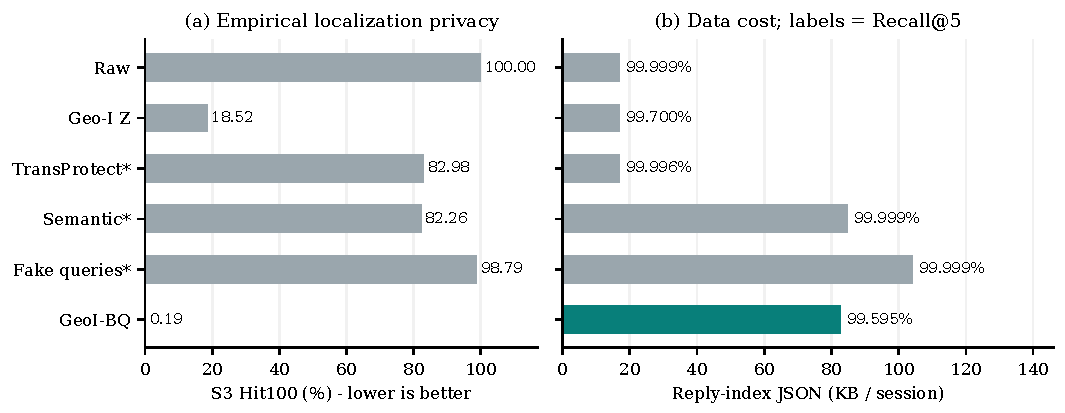
\includegraphics[width=\linewidth]{figures/privacy_utility_cost.pdf}
\caption{So sánh trên cùng cohort. Trái: S3 Hit100 thấp hơn có lợi cho privacy. Phải: reply-index JSON KB/phiên;
nhãn là session Recall@5. Đồ thị thể hiện ba mặt của đánh đổi, không gộp thành một score tùy ý. Dấu * chỉ adaptation.}
\label{fig:tradeoff}
\end{figure}
\Needspace{210pt}
\par\begingroup\small\setstretch{1.04}\setlength{\parskip}{0pt}
\begin{longtable}{@{}P{3.6cm}P{2.199cm}P{2.199cm}P{2.199cm}P{2.199cm}P{2.199cm}@{}}
\caption{Chi phí trung bình mỗi phiên 600 giây; KB = 1.000 byte}\label{tab:main-cost}\\
\toprule
\textbf{Phương pháp} & \textbf{Packet} & \textbf{Query điểm} & \textbf{Request KB} & \textbf{Reply KB} & \textbf{Sinh / tick ms} \\
\midrule\endfirsthead
\multicolumn{6}{l}{\small\textit{Bảng \thetable\ (tiếp)}}\\\toprule
\textbf{Phương pháp} & \textbf{Packet} & \textbf{Query điểm} & \textbf{Request KB} & \textbf{Reply KB} & \textbf{Sinh / tick ms} \\
\midrule\endhead
\midrule\multicolumn{6}{r}{\small\textit{Còn tiếp ở trang sau}}\\\endfoot
\bottomrule\endlastfoot
Raw GPS & 31{,}00 & 31{,}00 & 5{,}846 & 16{,}843 & <0{,}001 \\
Geo-I/REM Z (K1) & 31{,}00 & 31{,}00 & 6{,}352 & 16{,}921 & -- \\
TransProtect* & 31{,}00 & 31{,}00 & 6{,}351 & 16{,}847 & 3{,}287 \\
Semantic correlation* & 31{,}00 & 155{,}00 & 31{,}754 & 84{,}770 & 0{,}993 \\
Fake-query insertion* & 38{,}04 & 190{,}21 & 39{,}418 & 104{,}033 & 0{,}759 \\
\textbf{GeoI-BQ v1} & 31{,}00 & 155{,}00 & 31{,}756 & 82{,}557 & -- \\
\end{longtable}\endgroup\par

Trung bình mỗi phiên 600 s; KB = 1.000 byte. ``Query điểm'' đếm từng tọa độ, gồm mọi category theo cùng
provider API. Fake-query gửi trung bình 38,04 packets thay vì 31; mọi packet phụ đều được tính.
GeoI-BQ dùng 155 point queries, cùng mức K5 như Semantic* nhưng nhiều hơn singleton Z/TransProtect*.
Chi phí này giúp lấy ứng viên đủ rộng mà không gửi nhu cầu thật.

``Sinh/tick'' là tổng thời gian sinh adapter mới chia 31 input ticks; không là p95 hay latency end-to-end.
GeoI-BQ và REM-Z được replay từ outputs cũ nên không có generation timing đồng bộ trong trial này (ký hiệu --).
Service replay dùng shared warm cache và thứ tự chạy; không dùng nó để tuyên bố phương pháp nào nhanh hơn.
Byte chỉ gồm request/reply-index JSON, chưa gồm metadata POI đầy đủ, HTTP/TLS, mạng hay năng lượng thiết bị.


\subsection{Metrics gốc: giữ đúng hợp đồng}
\Needspace{210pt}
\par\begingroup\small\setstretch{1.04}\setlength{\parskip}{0pt}
\begin{longtable}{@{}P{3.7cm}P{2.179cm}P{2.179cm}P{2.179cm}P{2.179cm}P{2.179cm}@{}}
\caption{Metrics gốc áp dụng được và các trường hợp N/A}\label{tab:native}\\
\toprule
\textbf{Phương pháp} & \textbf{EIE S3 (m)} & \textbf{$\Delta c$ (m)} & \textbf{ASR} & \textbf{DER} & \textbf{Path count} \\
\midrule\endfirsthead
\multicolumn{6}{l}{\small\textit{Bảng \thetable\ (tiếp)}}\\\toprule
\textbf{Phương pháp} & \textbf{EIE S3 (m)} & \textbf{$\Delta c$ (m)} & \textbf{ASR} & \textbf{DER} & \textbf{Path count} \\
\midrule\endhead
\midrule\multicolumn{6}{r}{\small\textit{Còn tiếp ở trang sau}}\\\endfoot
\bottomrule\endlastfoot
Raw GPS & 0{,}0 & 0{,}00 & N/A & N/A & N/A \\
Geo-I/REM Z (K1) & 338{,}5 & 688{,}65 & N/A & N/A & N/A \\
TransProtect* & 54{,}4 & 47{,}44 & N/A & N/A & N/A \\
Semantic correlation* & 41{,}9 & N/A & N/A & N/A & N/A \\
Fake-query insertion* & 13{,}3 & N/A & N/A & N/A & N/A \\
\textbf{GeoI-BQ v1} & 2104{,}6 & N/A & N/A & N/A & N/A \\
\end{longtable}\endgroup\par

EIE cho point estimator ở S3 chính là MAE, không tạo thêm một kết quả độc lập. Với output singleton,
Eq.13 travel-cost distortion của TransProtect được đo bằng
\[
\Delta c=\sum_{d}\pi(d)\,|c(x,d)-c(y,d)|,
\]
với tám đích/prior chọn từ TRAIN, directed shortest-path metres và quy ước disconnected của provider.
Đây là \textbf{local-target proxy}: TransProtect* khoảng 47,44 m, REM-Z khoảng 688,65 m; không phải parity
với thí nghiệm Rome/SF gốc. Q-only hoặc real+dummy không có một released singleton $y$ duy nhất,
nên Eq.13 là N/A; không lấy centroid hoặc chọn Q gần GPS thật để tạo số.

ASR cần posterior calibrated trên real-member theo định nghĩa paper; DER cần hàm similarity và threshold
tương ứng; indistinguishable-path count cần bộ kiểm tra path đúng contract nguồn. Hiện chưa đủ đầu vào
để tính các metric này một cách đối chiếu được, vì vậy giữ N/A kèm lý do thay vì đổi tên Hit100 thành ASR.

\section{Mở rộng S4--S8: target phù hợp và phạm vi bằng chứng}\label{sec:extended-scenarios}
Phần này hợp nhất đánh giá ngày 09/11 vào cùng phương pháp và frozen outputs của so sánh chính.
Không sinh lại GPS/Q hoặc dùng một defense version khác cho các scenario còn lại. Vòng đầu gồm
66 tác vụ: sáu S4, 12 S5, 18 S6, sáu S7 và 24 S8. Vòng fusion S8 bổ sung 24 tác vụ. Tất cả tác vụ
hoàn tất, không có runtime failure. Một gate kiểm tra quá chặt được giữ riêng và phân tích phía dưới.

TRAIN/SELECTION/TEST vẫn là 20/8/20 family. S5/S6 dùng bootstrap 20 TEST family; S4/S8 dùng
10 block, mỗi block gồm hai family để giữ dependence của cặp âm hoặc unrelated partner. Có
10.000 bootstrap replicates với seed công khai 20261109. Đây là mở rộng trên cohort đã xem,
không là một phép confirmation ở thành phố mới. Utility toàn phiên cũ không được đổi nhãn thành
utility mới ở từng cutoff.

\subsection{S4: liên kết phiên, phân biệt với danh tính người và phương tiện}
Target trực tiếp là hai phiên ngày 7/8 có cùng route family hay không. Mỗi block/draw tạo hai cặp
cùng family và hai cặp chéo; TEST có 120 cặp cân bằng. Không dùng hai draws của cùng chuyến làm
hai phiên dương độc lập. Features đối xứng chỉ nhận coordinates/time; bank gồm
\textbf{ExtraTrees96, logistic, kNN-1/5}, distance thresholds và uniform. Thresholds được chọn trên
SELECTION, không chọn lại theo TEST.
\Needspace{210pt}
\par\begingroup\small\setstretch{1.04}\setlength{\parskip}{0pt}
\begin{longtable}{@{}P{3cm}P{4.052cm}P{4.052cm}P{4.052cm}@{}}
\caption{Liên kết phiên S4 ở mức route-family proxy}\label{tab:s4}\\
\toprule
\textbf{Phương pháp} & \textbf{BA\% [CI95\%]} & \textbf{AUC theo block [CI95\%]} & \textbf{Macro-F1} \\
\midrule\endfirsthead
\multicolumn{4}{l}{\small\textit{Bảng \thetable\ (tiếp)}}\\\toprule
\textbf{Phương pháp} & \textbf{BA\% [CI95\%]} & \textbf{AUC theo block [CI95\%]} & \textbf{Macro-F1} \\
\midrule\endhead
\midrule\multicolumn{4}{r}{\small\textit{Còn tiếp ở trang sau}}\\\endfoot
\bottomrule\endlastfoot
Raw GPS & 100{,}00 [100{,}00; 100{,}00] & 1{,}000 [1{,}000; 1{,}000] & 1{,}000 \\
REM-Z K1 & 91{,}67 [80{,}83; 98{,}33] & 0{,}956 [0{,}867; 1{,}000] & 0{,}916 \\
TransProtect* & 99{,}17 [97{,}50; 100{,}00] & 1{,}000 [1{,}000; 1{,}000] & 0{,}992 \\
Semantic correlation* & 100{,}00 [100{,}00; 100{,}00] & 1{,}000 [1{,}000; 1{,}000] & 1{,}000 \\
Fake-query insertion* & 93{,}33 [83{,}33; 100{,}00] & 1{,}000 [1{,}000; 1{,}000] & 0{,}933 \\
\textbf{GeoI-BQ v1} & 47{,}50 [40{,}00; 54{,}17] & 0{,}450 [0{,}386; 0{,}514] & 0{,}473 \\
\end{longtable}\endgroup\par


GeoI-BQ đạt BA 47,50\%, CI95\% [40,00;54,17], gần mốc cân bằng. Block-macro AUC là 0,450,
CI [0,386;0,514], trong khi pooled AUC là 0,442. Các controls có tín hiệu route-family association
mạnh hơn trong bank này. Không diễn giải AUC dưới 0,5 là bảo vệ hơn một hệ thống hoàn toàn độc lập;
đảo nhãn/xếp hạng và bất định mẫu phải được cân nhắc.

Cohort không cung cấp nhãn người và phương tiện vật lý độc lập với route family. Do đó
\textbf{person re-identification và vehicle re-identification còn N/A}. Kết quả ở đây chỉ hỗ trợ
một proxy liên kết trajectory. Account, device ID hoặc biển số không được giấu bởi việc tạo Q.
Hệ quả odds ở Chương~\ref{ch:method} là một phát biểu có điều kiện cho kênh suy luận, không thay
nhãn route-family bằng ground truth danh tính.

\subsection{S5: suy luận cạnh tương lai từ prefix}
Mỗi family có hai hình dạng cạnh/đích ứng viên là auxiliary context công khai. Target cạnh phải
xuất hiện lần đầu sau cutoff trong native SUMO. Hai clocks giữ nguyên là trước fork và cửa sổ
đang rẽ. Chỉ các packets đã phát tới cutoff được vào attacker, kể cả fake packets.
Bank gồm \textbf{candidate ExtraTrees96, kNN-1/5, curve/motion và uniform}; không cung cấp cạnh
thật hoặc trajectory sau cutoff như feature.
\Needspace{210pt}
\par\begingroup\small\setstretch{1.04}\setlength{\parskip}{0pt}
\begin{longtable}{@{}P{3.2cm}P{6.119cm}P{6.119cm}@{}}
\caption{S5: accuracy chọn cạnh tương lai trong hai ứng viên}\label{tab:s5}\\
\toprule
\textbf{Phương pháp} & \textbf{Trước fork: Acc\% [CI95\%]} & \textbf{Cửa sổ rẽ: Acc\% [CI95\%]} \\
\midrule\endfirsthead
\multicolumn{3}{l}{\small\textit{Bảng \thetable\ (tiếp)}}\\\toprule
\textbf{Phương pháp} & \textbf{Trước fork: Acc\% [CI95\%]} & \textbf{Cửa sổ rẽ: Acc\% [CI95\%]} \\
\midrule\endhead
\midrule\multicolumn{3}{r}{\small\textit{Còn tiếp ở trang sau}}\\\endfoot
\bottomrule\endlastfoot
Raw GPS & 50{,}00 [50{,}00; 50{,}00] & 50{,}00 [50{,}00; 50{,}00] \\
REM-Z K1 & 50{,}00 [50{,}00; 50{,}00] & 50{,}00 [50{,}00; 50{,}00] \\
TransProtect* & 50{,}00 [50{,}00; 50{,}00] & 50{,}00 [50{,}00; 50{,}00] \\
Semantic correlation* & 50{,}00 [50{,}00; 50{,}00] & 50{,}00 [50{,}00; 50{,}00] \\
Fake-query insertion* & 44{,}17 [38{,}33; 50{,}00] & 50{,}00 [43{,}33; 57{,}50] \\
\textbf{GeoI-BQ v1} & 52{,}50 [48{,}33; 57{,}50] & 50{,}83 [45{,}83; 55{,}83] \\
\end{longtable}\endgroup\par


Raw có accuracy 50\% ở cả hai pha. Clock native đang rẽ không bảo đảm đã có một packet GPS ở lane
rẽ: cadence 20 s bỏ lỡ cửa sổ ngắn trong TEST. Vì positive control chưa phân biệt được target,
GeoI-BQ gần 50\% không là bằng chứng rằng defense tạo ra phần khó suy luận đó. Toàn bộ family và
kết quả được giữ nguyên, không lọc lại để làm đối chứng hoặc proposed có score thuận lợi.
S5 hiện là diagnostic về observability; dự đoán next-route không giới hạn chưa được đánh giá.

\subsection{S6: chọn đích khi đã quan sát tín hiệu rẽ}
S6 bổ sung cutoff $20\lceil t_{\rm turn}/20\rceil$, mốc gửi đầu tiên từ clock đang rẽ trở đi.
Arrival của đích thật vẫn sau cutoff ở mọi row. Hai chuyến/family đi hai đích cân bằng; attacker
chọn trong hai đích đã biết bằng hình dạng/motion prefix. Đó là tác vụ đơn giản hóa có positive
control, không phải tìm một đích bất kỳ trong cả thành phố.
\Needspace{210pt}
\par\begingroup\small\setstretch{1.04}\setlength{\parskip}{0pt}
\begin{longtable}{@{}P{3.1cm}P{4.019cm}P{4.019cm}P{4.019cm}@{}}
\caption{S6 sau rẽ: chọn đích tương lai trong hai ứng viên}\label{tab:s6}\\
\toprule
\textbf{Phương pháp} & \textbf{Acc\% [CI95\%]} & \textbf{Hit100\% [CI95\%]} & \textbf{MAE m [CI95\%]} \\
\midrule\endfirsthead
\multicolumn{4}{l}{\small\textit{Bảng \thetable\ (tiếp)}}\\\toprule
\textbf{Phương pháp} & \textbf{Acc\% [CI95\%]} & \textbf{Hit100\% [CI95\%]} & \textbf{MAE m [CI95\%]} \\
\midrule\endhead
\midrule\multicolumn{4}{r}{\small\textit{Còn tiếp ở trang sau}}\\\endfoot
\bottomrule\endlastfoot
Raw GPS & 100{,}00 [100{,}00; 100{,}00] & 100{,}00 [100{,}00; 100{,}00] & 2{,}4 [2{,}4; 2{,}4] \\
REM-Z K1 & 50{,}00 [50{,}00; 50{,}00] & 50{,}00 [50{,}00; 50{,}00] & 572{,}7 [497{,}3; 647{,}8] \\
TransProtect* & 95{,}00 [90{,}83; 98{,}33] & 95{,}00 [90{,}83; 98{,}33] & 63{,}5 [17{,}7; 119{,}5] \\
Semantic correlation* & 95{,}00 [87{,}50; 100{,}00] & 95{,}00 [87{,}50; 100{,}00] & 63{,}9 [2{,}4; 156{,}2] \\
Fake-query insertion* & 99{,}17 [97{,}50; 100{,}00] & 99{,}17 [97{,}50; 100{,}00] & 11{,}3 [2{,}4; 29{,}1] \\
\textbf{GeoI-BQ v1} & 50{,}83 [44{,}17; 57{,}50] & 50{,}83 [44{,}17; 57{,}50] & 568{,}9 [458{,}8; 677{,}0] \\
\end{longtable}\endgroup\par


Raw đạt accuracy 100\%, các adaptation từ 95 tới 99,17\%. GeoI-BQ đạt 50,83\%, CI95\%
[44,17;57,50]; REM-Z là 50\%. Trong protocol này, Raw đã có tín hiệu mục tiêu nên kết quả có
giá trị phân biệt hơn S5. Hit100 trùng accuracy vì hai đích cách xa còn đích đúng cách native stop
chỉ vài mét. MAE 568,9 m của GeoI-BQ có CI [458,8;677,0], đo khoảng cách của \emph{đích ứng viên
đã chọn}, không phải sai số của một unrestricted destination regressor.

\begin{figure}[htbp]\centering
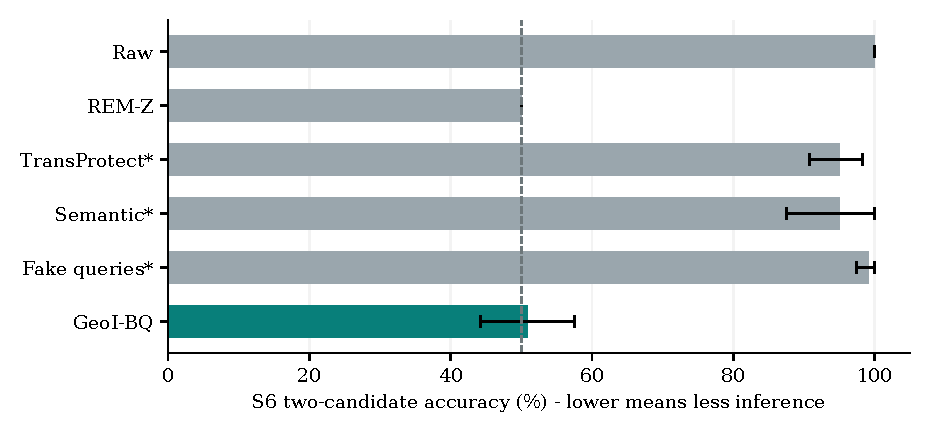
\includegraphics[width=\linewidth]{figures/future_choice.pdf}
\caption{S6 sau rẽ: accuracy chọn đích với CI95\%. Đường đứt là mốc uniform 50\% của hai lựa chọn.}
\label{fig:future}
\end{figure}

Hai task S5/S6 dùng cùng private route-choice bit trong workload; không được đếm như hai nguồn
bằng chứng hoàn toàn độc lập. Các pha, Brier và log loss đầy đủ ở Phụ lục~\ref{app:extended}.
Một tác vụ S6 dùng sáu chuyến lịch sử đã bảo vệ chưa chạy vì frozen outputs chỉ có ngày 7/8;
không dùng native lịch sử chưa bảo vệ để lấp vào như cùng contract.

\subsection{S7: kiểm tra payload có điều kiện}
Giữ cùng GPS/Q, clock và provider; thay bốn purposes nhân sáu categories tại local. Kiểm tra
\path{SessionCoverClient} thực qua provider probe trả reply rỗng cố định; actual frozen reply-mask
signatures được xác thực riêng. Đây là audit interface/payload, không chạy lại utility POI hoặc
huấn luyện một natural-intent attacker.
\Needspace{210pt}
\par\begingroup\small\setstretch{1.04}\setlength{\parskip}{0pt}
\begin{longtable}{@{}P{3.2cm}P{2.919cm}P{2.919cm}P{2.919cm}P{2.919cm}@{}}
\caption{S7: độ phân biệt payload có điều kiện trong common wrapper}\label{tab:s7}\\
\toprule
\textbf{Phương pháp} & \textbf{Wire bằng nhau} & \textbf{Purpose\%} & \textbf{Category\%} & \textbf{Joint\%} \\
\midrule\endfirsthead
\multicolumn{5}{l}{\small\textit{Bảng \thetable\ (tiếp)}}\\\toprule
\textbf{Phương pháp} & \textbf{Wire bằng nhau} & \textbf{Purpose\%} & \textbf{Category\%} & \textbf{Joint\%} \\
\midrule\endhead
\midrule\multicolumn{5}{r}{\small\textit{Còn tiếp ở trang sau}}\\\endfoot
\bottomrule\endlastfoot
Raw GPS & 100{,}00 & 25{,}00 & 16{,}67 & 4{,}17 \\
REM-Z K1 & 100{,}00 & 25{,}00 & 16{,}67 & 4{,}17 \\
TransProtect* & 100{,}00 & 25{,}00 & 16{,}67 & 4{,}17 \\
Semantic correlation* & 100{,}00 & 25{,}00 & 16{,}67 & 4{,}17 \\
Fake-query insertion* & 100{,}00 & 25{,}00 & 16{,}67 & 4{,}17 \\
\textbf{GeoI-BQ v1} & 100{,}00 & 25{,}00 & 16{,}67 & 4{,}17 \\
\end{longtable}\endgroup\par


Cả 1.056 streams đều có wire bằng nhau, tương ứng 25.344 counterfactuals. Với prior cân bằng,
conditional Bayes vulnerability là purpose 25\%, category 16,67\%, joint 4,17\%.
Control đưa purpose/category trực tiếp vào request khôi phục 100\% nhãn joint. Tất cả sáu arm dùng
chung cover wrapper, nên đây là tính chất của interface chung, không là ưu thế riêng của GeoI-BQ
trước implementation gốc của paper. Ý định gắn với tuyến, account hoặc lúc mở phiên vẫn có thể
được suy luận và chưa được đo ở đây.

\subsection{S8: hai kênh có prefix tương quan}
Dùng hai phiên native ngày 7/8 khác nhau cùng family, căn theo clock tương đối và cắt tại public
tick trước fork. GPS hai phiên giống nhau trên prefix đó. Attacker được cấp association giữa hai
kênh. Đây là \textbf{tương quan tổng hợp hoàn hảo sau căn clock}, không phải dữ liệu hai xe đồng
hành chạy đồng thời, cũng không là kết quả companion detection.

Bốn views là target-only, thêm protected partner, thêm Raw partner và thêm protected partner từ
family khác trong block. Target là GPS tại cutoff; mọi feature chỉ dùng causal prefix. Bảng dưới
dùng bank fusion V2, mỗi ô Hit100\% / MAE m; các loss được chọn attacker riêng.
\Needspace{210pt}
\par\begingroup\small\setstretch{1.04}\setlength{\parskip}{0pt}
\begin{longtable}{@{}P{3.2cm}P{2.919cm}P{2.919cm}P{2.919cm}P{2.919cm}@{}}
\caption{S8 với attacker fusion: Hit100 (\%) / MAE (m)}\label{tab:s8}\\
\toprule
\textbf{Phương pháp} & \textbf{Target} & \textbf{+ protected} & \textbf{+ raw} & \textbf{+ unrelated} \\
\midrule\endfirsthead
\multicolumn{5}{l}{\small\textit{Bảng \thetable\ (tiếp)}}\\\toprule
\textbf{Phương pháp} & \textbf{Target} & \textbf{+ protected} & \textbf{+ raw} & \textbf{+ unrelated} \\
\midrule\endhead
\midrule\multicolumn{5}{r}{\small\textit{Còn tiếp ở trang sau}}\\\endfoot
\bottomrule\endlastfoot
Raw GPS & 100{,}00 / 0{,}0 & 100{,}00 / 0{,}0 & 100{,}00 / 0{,}0 & 100{,}00 / 0{,}0 \\
REM-Z K1 & 10{,}83 / 359{,}7 & 6{,}67 / 300{,}8 & 100{,}00 / 0{,}0 & 10{,}83 / 359{,}7 \\
TransProtect* & 60{,}83 / 102{,}8 & 64{,}17 / 96{,}8 & 98{,}33 / 0{,}0 & 60{,}83 / 102{,}8 \\
Semantic correlation* & 45{,}00 / 101{,}4 & 75{,}00 / 46{,}2 & 100{,}00 / 0{,}0 & 45{,}00 / 101{,}4 \\
Fake-query insertion* & 16{,}67 / 1857{,}4 & 68{,}33 / 1857{,}4 & 100{,}00 / 0{,}0 & 16{,}67 / 1857{,}4 \\
\textbf{GeoI-BQ v1} & 0{,}00 / 2246{,}7 & 0{,}00 / 2226{,}8 & 100{,}00 / 0{,}0 & 0{,}00 / 2246{,}7 \\
\end{longtable}\endgroup\par


GeoI-BQ không có hit trong mẫu target/+protected, với MAE lần lượt 2.246,7 và 2.226,8 m.
Điều đó không chứng minh risk bằng không; bootstrap [0;0] khi mẫu toàn không-hit chỉ phản ánh
giới hạn của resampling mẫu đó. Khi Raw partner được cấp, estimator đọc partner trực tiếp có
Hit100 100\% ở mọi arm vì GPS prefix trùng nhau. Selected estimator TransProtect* đạt 98,33\%
Hit100 ở TEST, còn MAE 0 thuộc một estimator khác; các arm còn lại selected Hit100 là 100\%.
Không gộp hai selected losses thành một attacker duy nhất.

Kết quả cho thấy raw side information rất mạnh có thể làm mất vị trí mục tiêu dù target stream
đã bảo vệ. Một guard single-session không tự chứng nhận nhiều kênh/người cùng lúc. View unrelated
giúp kiểm tra rằng phép ghép ngẫu nhiên không tạo cùng tín hiệu; nó chưa mô hình hóa mọi dạng
tương quan mềm hoặc auxiliary data thực tế.

\subsection{Tăng cường attacker S8: giữ cả V1 và V2}
V1 có ExtraTrees64, kNN, prior, centroid/velocity và luôn giữ target-only estimators trong joint
bank. Sau khi xem V1, audit nhận ra còn thiếu phép fusion đơn giản. V2 giữ V1 rồi thêm trung bình
centroid/median/velocity hai kênh với trọng số $1/4,1/2,3/4$, midpoint của cặp Q gần nhất và trung
bình hai/ba cặp gần nhất. Nếu hai tập cùng chứa GPS thật, đối chiếu hai tập có thể lộ thành viên đó.
Không dùng GPS target, nhãn real/fake hoặc evaluator IDs để tìm cặp.
\Needspace{210pt}
\par\begingroup\small\setstretch{1.04}\setlength{\parskip}{0pt}
\begin{longtable}{@{}P{3.1cm}P{2.944cm}P{2.944cm}P{2.944cm}P{2.944cm}@{}}
\caption{S8 protected-partner: V1 và vòng attacker fusion V2}\label{tab:fusion}\\
\toprule
\textbf{Phương pháp} & \textbf{V1 Hit\%} & \textbf{V2 Hit\%} & \textbf{V1 MAE m} & \textbf{V2 MAE m} \\
\midrule\endfirsthead
\multicolumn{5}{l}{\small\textit{Bảng \thetable\ (tiếp)}}\\\toprule
\textbf{Phương pháp} & \textbf{V1 Hit\%} & \textbf{V2 Hit\%} & \textbf{V1 MAE m} & \textbf{V2 MAE m} \\
\midrule\endhead
\midrule\multicolumn{5}{r}{\small\textit{Còn tiếp ở trang sau}}\\\endfoot
\bottomrule\endlastfoot
Raw GPS & 100{,}00 & 100{,}00 & 0{,}0 & 0{,}0 \\
REM-Z K1 & 10{,}83 & 6{,}67 & 359{,}7 & 300{,}8 \\
TransProtect* & 60{,}83 & 64{,}17 & 102{,}8 & 96{,}8 \\
Semantic correlation* & 45{,}00 & 75{,}00 & 101{,}4 & 46{,}2 \\
Fake-query insertion* & 16{,}67 & 68{,}33 & 1857{,}4 & 1857{,}4 \\
\textbf{GeoI-BQ v1} & 0{,}00 & 0{,}00 & 2226{,}8 & 2226{,}8 \\
\end{longtable}\endgroup\par


Semantic* tăng Hit100 từ 45 lên 75\%; Fake-query* từ 16,67 lên 68,33\%. Điều này minh họa vì sao
một attacker bank thiếu thao tác cơ bản có thể làm defense trông mạnh hơn. REM-Z có MAE giảm nhưng
selected Hit100 cũng giảm ở TEST; selection đúng protocol không bảo đảm mọi loss TEST đều cải thiện.
V2 được chốt sau readout V1 và chọn trên SELECTION: đây là post-V1 diagnostic trên cùng dữ liệu
đã xem, không phải confirmation độc lập.

\begin{figure}[htbp]\centering
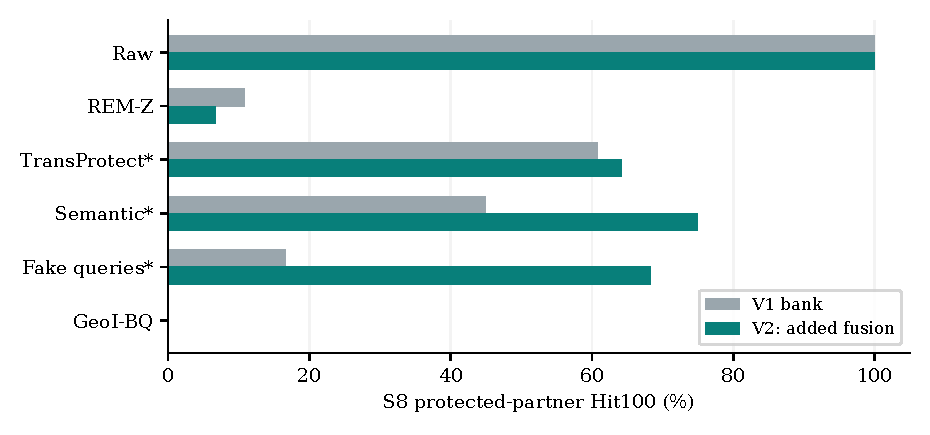
\includegraphics[width=\linewidth]{figures/joint_attack_fusion.pdf}
\caption{S8 protected-partner: readout V1 và V2. Fusion bổ sung làm rõ rủi ro giao hai tập chứa GPS thật.}
\label{fig:fusion}
\end{figure}

Verifier V2 ban đầu đặt gate selected Raw-partner Hit100 phải bằng 100\% ở mọi arm. Một fusion
estimator có tie tốt trên SELECTION chỉ đạt 98,33\% ở TransProtect* TEST; available
\path{partner_centroid} vẫn đạt 100\%. Giữ failure gốc và dùng checker độc lập kiểm tra cả available
control lẫn selected score. Không sửa predictions hoặc defense để thỏa gate sai. Chi tiết replay
ở Phụ lục~\ref{app:repro}.

\subsection{Tổng hợp mức hoàn thành theo scenario}
\begin{longtable}{@{}P{1cm}P{5.0cm}P{9.4cm}@{}}
\caption{Mức bằng chứng hiện có; không đồng nhất coverage với bảo vệ tuyệt đối.}\label{tab:scenario-status}\\
\toprule Case & Bằng chứng hiện có & Điều chưa được kết luận\\\midrule\endfirsthead
\toprule Case & Bằng chứng hiện có & Điều chưa được kết luận\\\midrule\endhead
\bottomrule\endfoot
S1 & Isolated-event Hit100/MAE & Không là chứng nhận mọi snapshot attacker.\\
S2 & Late-window coordinate proxy & Chưa suy luận semantic stop/home/work.\\
S3 & Whole-window reconstruction & Không là xác nhận ngoài cohort/thành phố.\\
S4 & Route-family association và odds có điều kiện & Nhãn người/xe vật lý, account anonymity còn N/A.\\
S5 & Causal two-edge diagnostic & Raw chance: chưa tách đóng góp defense.\\
S6 & Two-destination post-turn, Raw có tín hiệu & Unrestricted destination/routine history còn ngoài trial.\\
S7 & Conditional payload noninterference & Natural intent hoặc route-correlated purpose chưa đo.\\
S8 & Aligned correlated channels, bank fusion & Native co-travel, association detection và joint theorem riêng.\\
S9 & First GPS từ toàn transcript & Không dựa vào giấu public start clock.\\
S10 & Last GPS từ toàn transcript & Không dựa vào giấu end clock hoặc bỏ packet cuối bằng delay.\\
\end{longtable}

\section{Supporting analysis -- Giải thích các thành phần}
\subsection{Cache trên cùng output và provider tĩnh}
Current giữ packet hiện tại; epoch60 giữ metadata trong đoạn 60 s; session tích lũy cả phiên.
Các chế độ dùng cùng GPS/reference, không tạo Q mới. Đây là phép tách ảnh hưởng của bộ nhớ khỏi
ảnh hưởng của privacy kernel.
\Needspace{210pt}
\par\begingroup\small\setstretch{1.04}\setlength{\parskip}{0pt}
\begin{longtable}{@{}P{4cm}P{3.719cm}P{3.719cm}P{3.719cm}@{}}
\caption{Macro Recall@5 theo phạm vi cache trên cùng output}\label{tab:cache}\\
\toprule
\textbf{Phương pháp} & \textbf{Current (\%)} & \textbf{Epoch60 (\%)} & \textbf{Session (\%)} \\
\midrule\endfirsthead
\multicolumn{4}{l}{\small\textit{Bảng \thetable\ (tiếp)}}\\\toprule
\textbf{Phương pháp} & \textbf{Current (\%)} & \textbf{Epoch60 (\%)} & \textbf{Session (\%)} \\
\midrule\endhead
\midrule\multicolumn{4}{r}{\small\textit{Còn tiếp ở trang sau}}\\\endfoot
\bottomrule\endlastfoot
Raw GPS & 99{,}999 & 99{,}999 & 99{,}999 \\
Geo-I/REM Z (K1) & 98{,}610 & 98{,}610 & 99{,}700 \\
TransProtect* & 99{,}996 & 99{,}996 & 99{,}996 \\
Semantic correlation* & 99{,}999 & 99{,}999 & 99{,}999 \\
Fake-query insertion* & 99{,}999 & 99{,}999 & 99{,}999 \\
\textbf{GeoI-BQ v1} & 96{,}780 & 97{,}123 & 99{,}595 \\
\end{longtable}\endgroup\par


GeoI-BQ tăng từ 96,780\% current lên 97,123\% epoch60 và 99,595\% session. Cache giúp bù việc
không truy vấn trực tiếp GPS. Tuy nhiên, proof inclusion chỉ giữ ở cùng GPS/request và metadata
hợp lệ. Di chuyển sang một vùng khác có thể làm reference đổi; thông tin giờ mở cửa/giá/status
động có thể làm cache mất hiệu lực. Do đó kết quả session tĩnh không là chứng chỉ chất lượng
dịch vụ online động mà không có thêm chính sách expiry/refresh.

\subsection{Response depth và vai trò của GPS local}
Trên cùng Q/time và provider signatures, truncation L30 cho macro Recall 94,170\%, thấp hơn L60
5,425 điểm phần trăm, CI95\% [3,486;7,527]. Radius chịu chênh lệch lớn nhất, khoảng 10,374 điểm
phần trăm. Bảng chi tiết ở Phụ lục~\ref{app:support}; đây là replay/sensitivity có contract riêng,
không là một lần cải thiện privacy hoặc một thử nghiệm thành phố mới.

Một correction metadata đã đổi nhãn request nguồn cũ từ L30 sang L60 để khớp callback thực tế.
Nó không thay Q/time, reply masks, Recall hoặc độ dài bytes trong main trial. Cấu hình trình bày
hiện tại ghi L60 mỗi category/tọa độ; không nối score của L30 cũ với score mới thành một comparison
cùng cấu hình. Source hashes và verifier ghi lại correction này.

GPS local dùng đánh giá/ranking tại grid 20 s; lớp bảo vệ chỉ đưa private information mới vào
upstream theo pacing tối thiểu 60 s và cap. Vì vậy ít protected reads không đồng nghĩa điện thoại
chỉ bật GNSS từng ấy lần, cũng không chứng minh tiết kiệm pin. Đây là ranh giới giữa quan sát
của server và nhu cầu local, không phải một thí nghiệm năng lượng.

\subsection{Ablation public base và thích nghi theo belief}
Bảng ablation nội bộ ngày 14/10 giữ cùng frozen release ở Phụ lục~\ref{app:support}. Matched public
base $\Gamma=0$ đạt macro 99,711\%, cao hơn GeoI-BQ $\Gamma=1$ là 99,595\% trên workload này.
Service-cover đạt 100\% nhưng là control retrieval nội bộ, không phải một paper đối chứng.

Kết quả đó phù hợp với định lý utility: gain score không bắt buộc actual Recall gain. $\Gamma=0$
loại private adaptation của Q khi context cố định; vì thế nó cũng có Q-channel independence mạnh
hơn. Cohort này \textbf{chưa chứng minh belief adaptation cần thiết hoặc $\Gamma=1$ tối ưu}.
Thiết kế đề xuất cho phép bounded adaptation có accounting, còn giá trị thực tế của adaptation
trong catalogue lớn/động cần được xác nhận. Không thay baseline sau khi nhìn TEST để che kết quả này.

\section{Discussion -- Độ tin cậy và phạm vi kết luận}\label{sec:discussion}
\subsection{Mối quan hệ giữa chứng minh và benchmark}
Lý thuyết trả lời một câu hỏi khác với accuracy của một attack: các phân phối transcript được
phép khác nhau tới đâu khi private input đổi. Nếu một attacker mới mạnh hơn làm Hit100 tăng,
định lý kernel không tự bị phủ định; phải kiểm tra liệu attack/side channel có nằm trong model và
có vi phạm cận phân phối đã chứng minh không. Ngược lại, Hit thấp không đủ chứng nhận implementation
đúng kernel lý tưởng. Hai loại bằng chứng phải được đọc cùng giả thiết.

Với S1--S3/S9--S10, finite bank hiện tại cho thấy Q-only hạn chế định vị tốt hơn các controls/adaptations
trong cùng trial. Với S4/S6, có thêm bằng chứng tác vụ có target cụ thể. S5 chưa có positive control
đủ mạnh; S7 là conditional interface property chung; S8 là diagnostic tương quan tổng hợp và raw side
information. Không lấy việc đã có mười dòng scenario làm bằng chứng mười bài toán đều được giải quyết đầy đủ.

\subsection{Validity của phép so sánh phương pháp}
Các adaptation giữ ý tưởng cơ chế nhưng thay neural predictors hoặc nguồn semantic. Do đó conclusion
chỉ là controlled comparison của các implementation đã audit. Epsilon, output contracts và query
counts khác nhau; không nói cùng privacy budget hoặc cùng cost. Native metrics N/A phản ánh thiếu
contract tương ứng, không loại một result bất lợi. Cần author code, dữ liệu và task alignment trước
khi phát biểu superiority đối với kết quả chính thức của paper.

Raw control xác nhận năm coordinate targets có thể quan sát, nhưng S5 cho thấy control có thể không
cung cấp tín hiệu trong một cutoff cụ thể. S8 V2 cho thấy một bank học có thể thiếu fusion rất đơn giản.
Vì vậy attacker selection phải công khai, giữ loss-specific models và không trình bày số lớn ở MAE
như một chứng chỉ attacker tối ưu đã thất bại.

\subsection{Validity của dữ liệu và utility gần bão hòa}
Chia family tránh một dạng leakage giữa các chuyến cùng nhóm, nhưng bản đồ/cohort đã được xem trong
quá trình phát triển. TRAIN/SELECTION/TEST không biến nó thành một geography holdout độc lập. Native
SUMO phản ánh những ràng buộc giao thông của mạng đã xây, chưa đại diện hành vi người thật, quyết định
POI hay nhãn người/xe. Bootstrap family/block đo resampling của số nhóm hữu hạn đang có, không đo
tất cả nguồn domain shift.

Catalogue có 418 POI và sáu categories. K5 nhân L60 mỗi category có thể trả tối đa 1.800 entries trước
dedup ở một packet, nên coverage và session cache dễ gần bão hòa. Đây là lời giải thích quan trọng
cho Recall gần 100\%, không chỉ là đặc tính của planner. Nếu API cho tải toàn catalogue hợp lệ một
lần với cost chấp nhận được, client có thể giảm nhu cầu periodic coordinate queries; lợi thế của
planner khi đó phải được đánh giá lại theo chính contract đó. Không ghép số từ một diagnostic bulk
khác cohort/cấu hình vào bảng chính để chứng minh ưu thế.

Privacy MAE lớn cũng phụ thuộc public library rộng so với route workload. Công bố sự khác nhau này
giúp phân biệt guard lý thuyết với lợi ích do geometry hiện tại. Một nghiên cứu tiếp theo cần catalogue
lớn/động hơn, reference đầy đủ và những family mới chốt trước khi đánh giá.

\subsection{Giới hạn triển khai và tài nguyên}
Float Geo-I, entropy nguồn random và full-state restore là những điều kiện thực thi còn phải kiểm
chứng trước deployment có cam kết. Header/account/IP, kích thước payload không được giữ cố định,
click feedback và private start/stop timing có thể tạo kênh khác. Finite cap của một phiên không
xóa composition qua nhiều phiên liên kết hoặc qua người tương quan.

Chi phí hiện báo là counts và serialized index JSON. Metadata thực, network latency, server billing,
GNSS duty cycle và năng lượng chưa có phép đo đồng bộ. BQ/REM-Z được replay nên không có generation
timing cùng trial. Các giới hạn này không làm mất giá trị của counts đã kiểm chứng, nhưng ngăn kết
luận phương pháp nhanh hơn/rẻ hơn trên thiết bị người dùng.

\subsection{Kiểm chứng tái lập và failure accounting}
Main verifier kiểm tra độc lập 392.832 ô utility, 600 family-level privacy scores, 528 native-cost
trip values, 5.456 proposed prefixes và tổng 104.168 point queries trên toàn các split/arms.
Supplement kiểm tra split/block, future cutoffs, selectors, predictions, CIs và mọi fake packet.
Kết quả failure gate S8 ban đầu được giữ bên cạnh checker sửa điều kiện kiểm tra, không ghi đè
predictions. Cả ba benchmark folders và 108 frozen release pins được xác thực trước xuất bảng.

Quy trình này không biến dữ liệu đã xem thành dữ liệu mới hoặc làm mọi sai số biến mất. Nó bảo đảm
người review có thể đi từ kết luận về đúng con số, task, output và source dùng để tính. Trong luận
văn, đây là cơ sở để giới hạn contribution ở một phương pháp có đặc tả rõ, chuỗi chứng minh có điều
kiện và một đánh giá thực nghiệm có thể kiểm tra.

\chapter{Summary -- Kết luận}\label{ch:summary}
Luận văn xem trajectory privacy như một bài toán bảo vệ transcript dịch vụ theo thời gian. Một
tọa độ giả ở từng thời điểm chưa đủ: quyền quan sát cả chuỗi, quyết định cập nhật và tương quan
giữa các đầu ra đều cần được đặc tả. Đồng thời, utility được đánh giá bằng đáp án POI người dùng
thực nhận thay vì chỉ độ lệch giữa GPS và tọa độ phát.

\section{Trả lời các câu hỏi nghiên cứu}
\textbf{RQ1 -- Bảo đảm privacy toàn transcript.} GeoI-BQ v1 nối REM/noisy reuse với một prospective
cap cho private GPS và một guard riêng cho lựa chọn đoạn Q. Trên miền/support chung và các giả thiết
kernel, clock, ledger, provider đã nêu, chuỗi Q có tỷ số likelihood không quá $R_n\le e^{\Gamma_Q}$;
với $\Gamma_Q=1$, cận toàn thời lượng nhỏ hơn 2,437372. Nhánh Geo-I lý tưởng cho cận theo metric
trajectory; khi cả hai nhánh hợp lệ có thể lấy minimum của chúng. Đây là giới hạn mức transcript
làm thay đổi khả năng phân biệt/suy luận, không là chứng minh attacker không thể biết vị trí.

\textbf{RQ2 -- Utility và các điều kiện cần.} Centered kernel có gain không âm trên planning score,
còn actual utility gain phụ thuộc covariance/proxy calibration. Union/cache và local ranking giữ
được các reference POI đã truy hồi tại cùng GPS/request khi metadata hợp lệ. Phân tích toàn history
cho cận utility so matched public base bằng conditional expectation, không dùng IID. Floor chuyển
sang GPS thật vẫn cần bound sai số và provider completeness. Những điều kiện chưa chứng nhận không
được đặt bằng không trong kết luận.

\textbf{RQ3 -- Trade-off thực nghiệm.} Trong controlled comparison với ba adaptation đã audit từ
paper và Raw/REM-Z controls, GeoI-BQ đạt session Recall@5 99,595\%, CI95\% [99,224;99,903]. Các
coordinate tasks S1--S3/S9--S10 có Hit100 0--0,188\% dưới bank đã chọn, thấp hơn các adaptation trong
trial, đổi lại dùng 155 point queries mỗi phiên và utility thấp hơn khoảng 0,4 điểm phần trăm so
ba adaptation. Các con số không chứng minh mọi original paper implementation hoặc mọi attacker
đều thua, và không là generalization ngoài cohort.

\section{Đóng góp thực sự của bản hiện tại}
Thứ nhất, luận văn hệ thống hóa targets, output contracts và một protocol đánh giá bổ sung giữa
các cơ chế khác dạng. MAE, Recall và bootstrap là kiến thức kế thừa; đóng góp là cách ghép target,
window, aggregation, cost và failure accounting thành một phép đối chiếu kiểm tra được.

Thứ hai, phương pháp tách protected reference khỏi public query action, quản lý noisy reuse theo
phiên và chọn chung đoạn Q bằng kernel bị chặn có integer representation. Các chứng minh liên kết
từ thành phần đến transcript và nêu rõ điều kiện của suy luận Bayes cũng như utility. Không quy
đóng góp thành việc tạo thêm nhiễu hoặc phát minh lại Geo-I.

Thứ ba, artifact chứa main comparison, các tác vụ S4--S8 có scope riêng, bảng CIs/selected attackers,
source pins và verifier. Quá trình sửa attacker S8 được giữ để kết quả có thể bị kiểm tra và phản
biện. Đây là bằng chứng bổ sung cho thiết kế, không thay cho các giả thiết toán học.

\section{Giới hạn và hướng phát triển}
Ưu tiên tiếp theo là chứng nhận sampler upstream/restore toàn state và nguồn randomness; sau đó
đánh giá trên cohort/bản đồ mới và catalogue lớn/động với latency, bytes metadata đầy đủ và energy
thực đo. Matched public base đang có utility tốt hơn trên cohort hiện tại, nên cần xác định điều
kiện nào private adaptation thực sự đáng chi phí thay vì mặc định $\Gamma=1$ tối ưu.

Identity người/xe cần nhãn vật lý và task riêng; route-family association chưa đủ. S5 cần cadence
và positive control phù hợp; S6 cần lựa chọn/historical context đa dạng hơn. S7 cần đo route-correlated
intent ngoài payload, S8 cần dữ liệu tương quan thực và phân tích joint channels/multiple sessions.
Các hướng đó mở rộng phạm vi đã có, không được trình bày như kết quả hoàn thành trong bản này.

Bản hiện tại cung cấp một cơ sở thống nhất để review: kiến trúc/đặc tả trước, chứng minh có điều kiện
tiếp theo, rồi benchmark cùng protocol và kết luận tương xứng. Từ đó có thể chỉnh sửa diễn giải,
củng cố chứng nhận triển khai và xác nhận ngoài miền mà vẫn giữ nền tảng Geo-I của phương pháp.

\begin{small}\raggedright\begin{thebibliography}{99}
\addcontentsline{toc}{chapter}{References -- Tài liệu tham khảo}
\bibitem{transprotect} S. Yadav, C. Yu, X. Xie, Y. Huang và C. Qiu. Protecting Vehicle Location Privacy with Contextually-Driven Synthetic Location Generation. ACM SIGSPATIAL 2024. \href{https://arxiv.org/abs/2409.09495}{DOI: 10.1145/3678717.3691211}.
\bibitem{semantic} H. Liu, H. Peng và N. Zhou. A dummy-based location privacy protection scheme with semantic correlation of moving paths. Journal of King Saud University Computer and Information Sciences 38:478. 2026. \href{https://link.springer.com/article/10.1007/s44443-026-00899-w}{DOI: 10.1007/s44443-026-00899-w}.
\bibitem{fake} H. Liu, S. Hu và N. Zhou. Location privacy protection in continuous LBSs: enhancing anonymity via fake queries. Journal of King Saud University Computer and Information Sciences 38:53. 2026. \href{https://link.springer.com/article/10.1007/s44443-025-00438-z}{DOI: 10.1007/s44443-025-00438-z}.
\bibitem{ev} U. I. Atmaca, S. Biswas, C. Maple và C. Palamidessi. A privacy-preserving querying mechanism with high utility for electric vehicles. IEEE Open Journal of Vehicular Technology 5:262--277. 2024. \href{https://wrap.warwick.ac.uk/id/eprint/183198/}{DOI: 10.1109/OJVT.2024.3360302}.
\bibitem{cpcrok} J. Wang, H. Li, Y. Sun, C. Phillips, A. Mylonas và D. Gritzalis. CPCROK: A Communication-Efficient and Privacy-Preserving Scheme for Low-Density Vehicular Ad Hoc Networks. Future Internet 17(4):165. 2025. \href{https://uhra.herts.ac.uk/id/eprint/25705/}{DOI: 10.3390/fi17040165}.
\bibitem{dpfetc} B. Yue, S. Li, A. Liu và X. Li. DP-FETC: a differentially private trajectory publishing method based on feature extraction and trajectory correlation. Electronic Research Archive 33(11):6631--6651. 2025. \href{https://www.aimspress.com/article/doi/10.3934/era.2025293}{DOI: 10.3934/era.2025293}.
\bibitem{ptppm} M. Min và cộng sự. Road Network-Aware Personalized Trajectory Protection with Differential Privacy under Spatiotemporal Correlations. arXiv:2511.21020, preprint. 2025. \href{https://arxiv.org/abs/2511.21020}{DOI: 10.48550/arXiv.2511.21020}.
\bibitem{sok} E. Buchholz, A. Abuadbba, S. Wang, S. Nepal và S. S. Kanhere. SoK: Can Trajectory Generation Combine Privacy and Utility?. Proceedings on Privacy Enhancing Technologies 2024(3):75--93. \href{https://petsymposium.org/popets/2024/popets-2024-0068.pdf}{DOI: 10.56553/popets-2024-0068}.
\bibitem{geoi} M. E. Andrés, N. E. Bordenabe, K. Chatzikokolakis và C. Palamidessi. Geo-Indistinguishability: Differential Privacy for Location-Based Systems. ACM CCS 2013, pp.901--914. \href{https://arxiv.org/abs/1212.1984}{Nguồn tác giả}.
\bibitem{predictive} K. Chatzikokolakis, C. Palamidessi và M. Stronati. A Predictive Differentially-Private Mechanism for Mobility Traces. Privacy Enhancing Technologies 2014. \href{https://petsymposium.org/2014/papers/Chatzikokolakis.pdf}{Nguồn tác giả}.
\bibitem{dworkroth} C. Dwork và A. Roth. The Algorithmic Foundations of Differential Privacy. Foundations and Trends in Theoretical Computer Science 9(3--4), 211--407, 2014. \href{https://doi.org/10.1561/0400000042}{doi:10.1561/0400000042}. Bản tác giả: \url{https://www.cis.upenn.edu/~aaroth/Papers/privacybook.pdf}.
\bibitem{mobilityunique} Y.-A. de Montjoye, C. A. Hidalgo, M. Verleysen và V. D. Blondel. Unique in the Crowd: The privacy bounds of human mobility. Scientific Reports 3, 1376, 2013. \href{https://doi.org/10.1038/srep01376}{doi:10.1038/srep01376}.
\bibitem{sumo} P. Alvarez Lopez, M. Behrisch, L. Bieker-Walz, J. Erdmann, Y.-P. Flötteröd, R. Hilbrich, L. Lücken, J. Rummel, P. Wagner và E. Wießner. Microscopic Traffic Simulation using SUMO. IEEE ITSC, 2575--2582, 2018. \href{https://doi.org/10.1109/ITSC.2018.8569938}{doi:10.1109/ITSC.2018.8569938}. Nguồn hướng dẫn trích dẫn: \url{https://sumo.dlr.de/docs/FAQ.html}.
\bibitem{osm} OpenStreetMap contributors. OpenStreetMap: Copyright and License. \url{https://www.openstreetmap.org/copyright/}. Truy cập 09/11/2026; nguồn địa lý được lưu theo snapshot trong repository.
\bibitem{mironov} I. Mironov. On Significance of the Least Significant Bits for Differential Privacy. ACM CCS, 650--661, 2012. \href{https://doi.org/10.1145/2382196.2382264}{doi:10.1145/2382196.2382264}. Nguồn tác giả: \url{https://www.microsoft.com/en-us/research/publication/on-significance-of-the-least-significant-bits-for-differential-privacy/}.
\bibitem{efron} B. Efron. Bootstrap Methods: Another Look at the Jackknife. The Annals of Statistics 7(1), 1--26, 1979. \href{https://doi.org/10.1214/aos/1176344552}{doi:10.1214/aos/1176344552}.
\bibitem{extratrees} P. Geurts, D. Ernst và L. Wehenkel. Extremely randomized trees. Machine Learning 63, 3--42, 2006. \href{https://doi.org/10.1007/s10994-006-6226-1}{doi:10.1007/s10994-006-6226-1}.

\end{thebibliography}\end{small}
\appendix
\chapter{CIs và attacker của so sánh chính}\label{app:main-ci}
Các bảng dưới mở rộng bảng chính, không tạo trial mới. CI95\% theo 20 TEST families, 10.000
bootstrap replicates; các draws/trips được gộp trong family trước resampling. Hit100 và MAE chọn
model riêng trên SELECTION. Việc hai số trong một ô đến từ hai estimators không phải ensemble
được chọn sau TEST.
\section{Privacy: toàn bộ khoảng tin cậy}
\par\begingroup\footnotesize\setstretch{1.04}\setlength{\parskip}{0pt}
\begin{longtable}{@{}P{3.4cm}P{.7cm}P{2.624cm}P{2.624cm}P{2.624cm}P{2.624cm}@{}}
\caption{CI95\% đầy đủ cho năm tác vụ định vị/tái dựng}\label{tab:privacy-ci}\\
\toprule
\textbf{Phương pháp} & \textbf{S} & \textbf{Hit100\%} & \textbf{CI95\% Hit} & \textbf{MAE m} & \textbf{CI95\% MAE} \\
\midrule\endfirsthead
\multicolumn{6}{l}{\small\textit{Bảng \thetable\ (tiếp)}}\\\toprule
\textbf{Phương pháp} & \textbf{S} & \textbf{Hit100\%} & \textbf{CI95\% Hit} & \textbf{MAE m} & \textbf{CI95\% MAE} \\
\midrule\endhead
\midrule\multicolumn{6}{r}{\small\textit{Còn tiếp ở trang sau}}\\\endfoot
\bottomrule\endlastfoot
Raw GPS & S1 & 100{,}000 & [100{,}000; 100{,}000] & 0{,}0 & [0{,}0; 0{,}0] \\
Raw GPS & S2 & 100{,}000 & [100{,}000; 100{,}000] & 0{,}0 & [0{,}0; 0{,}0] \\
Raw GPS & S3 & 100{,}000 & [100{,}000; 100{,}000] & 0{,}0 & [0{,}0; 0{,}0] \\
Raw GPS & S9 & 100{,}000 & [100{,}000; 100{,}000] & 0{,}0 & [0{,}0; 0{,}0] \\
Raw GPS & S10 & 100{,}000 & [100{,}000; 100{,}000] & 0{,}0 & [0{,}0; 0{,}0] \\
Geo-I/REM Z (K1) & S1 & 18{,}522 & [14{,}892; 22{,}204] & 338{,}5 & [319{,}0; 359{,}8] \\
Geo-I/REM Z (K1) & S2 & 37{,}500 & [29{,}167; 45{,}833] & 214{,}3 & [171{,}2; 261{,}2] \\
Geo-I/REM Z (K1) & S3 & 18{,}522 & [14{,}892; 22{,}204] & 338{,}5 & [319{,}0; 359{,}8] \\
Geo-I/REM Z (K1) & S9 & 5{,}833 & [2{,}500; 10{,}000] & 435{,}8 & [380{,}2; 498{,}0] \\
Geo-I/REM Z (K1) & S10 & 35{,}000 & [26{,}667; 43{,}333] & 246{,}8 & [201{,}5; 297{,}8] \\
TransProtect* & S1 & 82{,}984 & [79{,}973; 85{,}672] & 54{,}4 & [47{,}9; 62{,}0] \\
TransProtect* & S2 & 94{,}167 & [88{,}333; 98{,}333] & 28{,}7 & [20{,}4; 39{,}1] \\
TransProtect* & S3 & 82{,}984 & [79{,}973; 85{,}672] & 54{,}4 & [47{,}9; 62{,}0] \\
TransProtect* & S9 & 96{,}667 & [92{,}500; 100{,}000] & 17{,}8 & [8{,}5; 29{,}3] \\
TransProtect* & S10 & 90{,}833 & [84{,}167; 96{,}667] & 33{,}6 & [23{,}2; 46{,}6] \\
Semantic correlation* & S1 & 82{,}258 & [77{,}097; 86{,}532] & 41{,}9 & [38{,}1; 46{,}1] \\
Semantic correlation* & S2 & 100{,}000 & [100{,}000; 100{,}000] & 8{,}2 & [5{,}1; 13{,}0] \\
Semantic correlation* & S3 & 82{,}258 & [77{,}097; 86{,}532] & 41{,}9 & [38{,}1; 46{,}1] \\
Semantic correlation* & S9 & 100{,}000 & [100{,}000; 100{,}000] & 5{,}3 & [5{,}0; 5{,}8] \\
Semantic correlation* & S10 & 100{,}000 & [100{,}000; 100{,}000] & 7{,}3 & [5{,}4; 10{,}6] \\
Fake-query insertion* & S1 & 53{,}387 & [41{,}156; 65{,}215] & 1213{,}0 & [907{,}7; 1539{,}9] \\
Fake-query insertion* & S2 & 92{,}500 & [85{,}000; 99{,}167] & 239{,}1 & [44{,}8; 481{,}7] \\
Fake-query insertion* & S3 & 98{,}790 & [97{,}957; 99{,}462] & 13{,}3 & [9{,}8; 18{,}5] \\
Fake-query insertion* & S9 & 99{,}167 & [97{,}500; 100{,}000] & 42{,}2 & [4{,}8; 116{,}4] \\
Fake-query insertion* & S10 & 100{,}000 & [100{,}000; 100{,}000] & 6{,}4 & [5{,}2; 7{,}9] \\
\textbf{GeoI-BQ v1} & S1 & 0{,}188 & [0{,}000; 0{,}565] & 2104{,}6 & [1784{,}5; 2436{,}0] \\
\textbf{GeoI-BQ v1} & S2 & 0{,}000 & [0{,}000; 0{,}000] & 2124{,}2 & [1789{,}4; 2462{,}4] \\
\textbf{GeoI-BQ v1} & S3 & 0{,}188 & [0{,}000; 0{,}565] & 2104{,}6 & [1784{,}5; 2436{,}0] \\
\textbf{GeoI-BQ v1} & S9 & 0{,}000 & [0{,}000; 0{,}000] & 1986{,}4 & [1626{,}2; 2343{,}0] \\
\textbf{GeoI-BQ v1} & S10 & 0{,}000 & [0{,}000; 0{,}000] & 2124{,}2 & [1789{,}4; 2462{,}4] \\
\end{longtable}\endgroup\par

\section{Utility: CI theo purpose và chênh lệch}
\Needspace{210pt}
\par\begingroup\small\setstretch{1.04}\setlength{\parskip}{0pt}
\begin{longtable}{@{}P{3.2cm}P{3.985cm}P{3.985cm}P{3.985cm}@{}}
\caption{Recall GeoI-BQ theo purpose và chênh lệch so với TransProtect*}\label{tab:purpose-ci}\\
\toprule
\textbf{Purpose} & \textbf{BQ Recall (\%)} & \textbf{CI95\% tuyệt đối} & \textbf{Δ so TransProtect* (pp), CI95\%} \\
\midrule\endfirsthead
\multicolumn{4}{l}{\small\textit{Bảng \thetable\ (tiếp)}}\\\toprule
\textbf{Purpose} & \textbf{BQ Recall (\%)} & \textbf{CI95\% tuyệt đối} & \textbf{Δ so TransProtect* (pp), CI95\%} \\
\midrule\endhead
\midrule\multicolumn{4}{r}{\small\textit{Còn tiếp ở trang sau}}\\\endfoot
\bottomrule\endlastfoot
Trung bình & 99{,}595 & [99{,}224; 99{,}903] & -0{,}401; [-0{,}773; -0{,}093] \\
Gần nhất & 99{,}638 & [99{,}280; 99{,}930] & -0{,}362; [-0{,}720; -0{,}070] \\
Nhanh nhất & 99{,}641 & [99{,}285; 99{,}930] & -0{,}359; [-0{,}715; -0{,}070] \\
Bán kính & 99{,}388 & [98{,}676; 99{,}894] & -0{,}612; [-1{,}324; -0{,}106] \\
Ít vòng đường & 99{,}712 & [99{,}362; 99{,}946] & -0{,}273; [-0{,}622; -0{,}040] \\
\end{longtable}\endgroup\par

\par\begingroup\small\setstretch{1.04}\setlength{\parskip}{0pt}
\begin{longtable}{@{}P{3.5cm}P{2.4cm}P{4.628cm}P{4.628cm}@{}}
\caption{Chênh lệch Recall theo purpose: GeoI-BQ trừ đối chứng}\label{tab:purpose-deltas}\\
\toprule
\textbf{Đối chứng} & \textbf{Purpose} & \textbf{BQ trừ control (pp)} & \textbf{CI95\% (pp)} \\
\midrule\endfirsthead
\multicolumn{4}{l}{\small\textit{Bảng \thetable\ (tiếp)}}\\\toprule
\textbf{Đối chứng} & \textbf{Purpose} & \textbf{BQ trừ control (pp)} & \textbf{CI95\% (pp)} \\
\midrule\endhead
\midrule\multicolumn{4}{r}{\small\textit{Còn tiếp ở trang sau}}\\\endfoot
\bottomrule\endlastfoot
Raw GPS & Trung bình & -0{,}404 & [-0{,}775; -0{,}095] \\
Raw GPS & Gần nhất & -0{,}362 & [-0{,}720; -0{,}070] \\
Raw GPS & Nhanh nhất & -0{,}359 & [-0{,}715; -0{,}070] \\
Raw GPS & Bán kính & -0{,}612 & [-1{,}324; -0{,}106] \\
Raw GPS & Ít vòng đường & -0{,}282 & [-0{,}634; -0{,}047] \\
Geo-I/REM Z (K1) & Trung bình & -0{,}105 & [-0{,}542; 0{,}275] \\
Geo-I/REM Z (K1) & Gần nhất & -0{,}114 & [-0{,}524; 0{,}241] \\
Geo-I/REM Z (K1) & Nhanh nhất & -0{,}112 & [-0{,}519; 0{,}242] \\
Geo-I/REM Z (K1) & Bán kính & -0{,}237 & [-1{,}006; 0{,}338] \\
Geo-I/REM Z (K1) & Ít vòng đường & 0{,}044 & [-0{,}381; 0{,}389] \\
TransProtect* & Trung bình & -0{,}401 & [-0{,}773; -0{,}093] \\
TransProtect* & Gần nhất & -0{,}362 & [-0{,}720; -0{,}070] \\
TransProtect* & Nhanh nhất & -0{,}359 & [-0{,}715; -0{,}070] \\
TransProtect* & Bán kính & -0{,}612 & [-1{,}324; -0{,}106] \\
TransProtect* & Ít vòng đường & -0{,}273 & [-0{,}622; -0{,}040] \\
Semantic correlation* & Trung bình & -0{,}404 & [-0{,}775; -0{,}096] \\
Semantic correlation* & Gần nhất & -0{,}362 & [-0{,}720; -0{,}070] \\
Semantic correlation* & Nhanh nhất & -0{,}359 & [-0{,}715; -0{,}070] \\
Semantic correlation* & Bán kính & -0{,}612 & [-1{,}324; -0{,}106] \\
Semantic correlation* & Ít vòng đường & -0{,}285 & [-0{,}637; -0{,}050] \\
Fake-query insertion* & Trung bình & -0{,}404 & [-0{,}775; -0{,}096] \\
Fake-query insertion* & Gần nhất & -0{,}362 & [-0{,}720; -0{,}070] \\
Fake-query insertion* & Nhanh nhất & -0{,}359 & [-0{,}715; -0{,}070] \\
Fake-query insertion* & Bán kính & -0{,}612 & [-1{,}324; -0{,}106] \\
Fake-query insertion* & Ít vòng đường & -0{,}285 & [-0{,}635; -0{,}051] \\
\end{longtable}\endgroup\par

\section{Toàn bộ selected attackers}
Tên model giữ đúng artifact để tra lại feature/selector. Đối với method Q-only, Z nội bộ không
thuộc attacker input. Shadow models là mô hình do protocol huấn luyện trên TRAIN, không phải
attack implementation được tuyên bố lấy nguyên từ paper nguồn.
\par\begingroup\footnotesize\setstretch{1.04}\setlength{\parskip}{0pt}
\begin{longtable}{@{}P{3.1cm}P{.7cm}P{5.678cm}P{5.678cm}@{}}
\caption{Toàn bộ attacker thực sự được chọn trong trial chính}\label{tab:main-selected}\\
\toprule
\textbf{Phương pháp} & \textbf{S} & \textbf{Attacker Hit100} & \textbf{Attacker MAE} \\
\midrule\endfirsthead
\multicolumn{4}{l}{\small\textit{Bảng \thetable\ (tiếp)}}\\\toprule
\textbf{Phương pháp} & \textbf{S} & \textbf{Attacker Hit100} & \textbf{Attacker MAE} \\
\midrule\endhead
\midrule\multicolumn{4}{r}{\small\textit{Còn tiếp ở trang sau}}\\\endfoot
\bottomrule\endlastfoot
Raw GPS & S1 & \path{centroid} & \path{centroid} \\
Raw GPS & S2 & \path{centroid} & \path{centroid} \\
Raw GPS & S3 & \path{centroid} & \path{centroid} \\
Raw GPS & S9 & \path{centroid} & \path{centroid} \\
Raw GPS & S10 & \path{centroid} & \path{centroid} \\
Geo-I/REM Z (K1) & S1 & \path{centroid} & \path{centroid} \\
Geo-I/REM Z (K1) & S2 & \path{centroid} & \path{centroid} \\
Geo-I/REM Z (K1) & S3 & \path{centroid} & \path{centroid} \\
Geo-I/REM Z (K1) & S9 & \path{centroid} & \path{centroid} \\
Geo-I/REM Z (K1) & S10 & \path{centroid} & \path{geometry_nearest_slot0_ols3_boundary} \\
TransProtect* & S1 & \path{centroid} & \path{centroid} \\
TransProtect* & S2 & \path{centroid} & \path{centroid} \\
TransProtect* & S3 & \path{centroid} & \path{centroid} \\
TransProtect* & S9 & \path{centroid} & \path{geometry_nearest_slot0_ols2_boundary} \\
TransProtect* & S10 & \path{geometry_nearest_slot0_ols6_boundary} & \path{geometry_nearest_slot0_ols6_boundary} \\
Semantic correlation* & S1 & \path{centroid} & \path{query_prior} \\
Semantic correlation* & S2 & \path{centroid} & \path{median} \\
Semantic correlation* & S3 & \path{centroid} & \path{query_prior} \\
Semantic correlation* & S9 & \path{centroid} & \path{observed_slots_slot4_ols2_boundary} \\
Semantic correlation* & S10 & \path{centroid} & \path{observed_slots_slot4_endpoint} \\
Fake-query insertion* & S1 & \path{query_prior} & \path{shadow_tree} \\
Fake-query insertion* & S2 & \path{viterbi_motion} & \path{viterbi_motion} \\
Fake-query insertion* & S3 & \path{viterbi_motion} & \path{viterbi_motion} \\
Fake-query insertion* & S9 & \path{public_boundary_viterbi_ols2} & \path{public_boundary_viterbi_ols2} \\
Fake-query insertion* & S10 & \path{public_boundary_viterbi_ols2} & \path{viterbi_motion} \\
\textbf{GeoI-BQ v1} & S1 & \path{centroid} & \path{shadow_prior_median} \\
\textbf{GeoI-BQ v1} & S2 & \path{centroid} & \path{shadow_prior_median} \\
\textbf{GeoI-BQ v1} & S3 & \path{centroid} & \path{shadow_prior_median} \\
\textbf{GeoI-BQ v1} & S9 & \path{centroid} & \path{geometry_nearest_prior_median} \\
\textbf{GeoI-BQ v1} & S10 & \path{centroid} & \path{geometry_nearest_prior_median} \\
\end{longtable}\endgroup\par


\chapter{Chi tiết các tác vụ bổ sung}\label{app:extended}
\section{S5: hai pha causal và calibration}
Accuracy chọn đúng candidate edge; Brier/log loss theo probability lớp 1. Native edge first occurrence
phải ở tương lai so cutoff. Raw chance ở cả hai pha là hạn chế của observability trong readout này.
\par\begingroup\small\setstretch{1.04}\setlength{\parskip}{0pt}
\begin{longtable}{@{}P{3cm}P{2.1cm}P{7.775cm} P{1cm}P{1cm}@{}}
\caption{Tất cả pha S5, xác suất dự đoán và CI}\label{tab:s5-full}\\
\toprule
\textbf{Phương pháp} & \textbf{Pha} & \textbf{Acc\% [CI95\%]} & \textbf{Brier} & \textbf{Log loss} \\
\midrule\endfirsthead
\multicolumn{5}{l}{\small\textit{Bảng \thetable\ (tiếp)}}\\\toprule
\textbf{Phương pháp} & \textbf{Pha} & \textbf{Acc\% [CI95\%]} & \textbf{Brier} & \textbf{Log loss} \\
\midrule\endhead
\midrule\multicolumn{5}{r}{\small\textit{Còn tiếp ở trang sau}}\\\endfoot
\bottomrule\endlastfoot
Raw GPS & Trước fork & 50{,}00 [50{,}00; 50{,}00] & 0{,}250 & 0{,}693 \\
Raw GPS & Cửa sổ rẽ & 50{,}00 [50{,}00; 50{,}00] & 0{,}250 & 0{,}693 \\
REM-Z K1 & Trước fork & 50{,}00 [50{,}00; 50{,}00] & 0{,}250 & 0{,}693 \\
REM-Z K1 & Cửa sổ rẽ & 50{,}00 [50{,}00; 50{,}00] & 0{,}250 & 0{,}693 \\
TransProtect* & Trước fork & 50{,}00 [50{,}00; 50{,}00] & 0{,}250 & 0{,}693 \\
TransProtect* & Cửa sổ rẽ & 50{,}00 [50{,}00; 50{,}00] & 0{,}250 & 0{,}693 \\
Semantic correlation* & Trước fork & 50{,}00 [50{,}00; 50{,}00] & 0{,}250 & 0{,}693 \\
Semantic correlation* & Cửa sổ rẽ & 50{,}00 [50{,}00; 50{,}00] & 0{,}252 & 0{,}697 \\
Fake-query insertion* & Trước fork & 44{,}17 [38{,}33; 50{,}00] & 0{,}315 & 0{,}853 \\
Fake-query insertion* & Cửa sổ rẽ & 50{,}00 [43{,}33; 57{,}50] & 0{,}373 & 5{,}372 \\
\textbf{GeoI-BQ v1} & Trước fork & 52{,}50 [48{,}33; 57{,}50] & 0{,}259 & 0{,}712 \\
\textbf{GeoI-BQ v1} & Cửa sổ rẽ & 50{,}83 [45{,}83; 55{,}83] & 0{,}259 & 0{,}714 \\
\end{longtable}\endgroup\par

\section{S6: tất cả pha và sai số đích}
Ba pha là trước fork, cửa sổ rẽ và tick gửi đầu từ cửa sổ rẽ trở đi. Arrival đích thật sau cutoff;
không dùng cả chuyến hoàn tất như observation rồi gọi bài toán đó là dự đoán tương lai.
\par\begingroup\footnotesize\setstretch{1.04}\setlength{\parskip}{0pt}
\begin{longtable}{@{}P{3cm}P{2.1cm}P{3.747cm} P{1cm}P{1cm}P{3.747cm}@{}}
\caption{Tất cả pha S6, xác suất dự đoán và sai số đích}\label{tab:s6-full}\\
\toprule
\textbf{Phương pháp} & \textbf{Pha} & \textbf{Acc\% [CI95\%]} & \textbf{Brier} & \textbf{Log loss} & \textbf{MAE m [CI95\%]} \\
\midrule\endfirsthead
\multicolumn{6}{l}{\small\textit{Bảng \thetable\ (tiếp)}}\\\toprule
\textbf{Phương pháp} & \textbf{Pha} & \textbf{Acc\% [CI95\%]} & \textbf{Brier} & \textbf{Log loss} & \textbf{MAE m [CI95\%]} \\
\midrule\endhead
\midrule\multicolumn{6}{r}{\small\textit{Còn tiếp ở trang sau}}\\\endfoot
\bottomrule\endlastfoot
Raw GPS & Trước fork & 50{,}00 [50{,}00; 50{,}00] & 0{,}250 & 0{,}693 & 572{,}7 [497{,}3; 647{,}8] \\
Raw GPS & Cửa sổ rẽ & 50{,}00 [50{,}00; 50{,}00] & 0{,}250 & 0{,}693 & 572{,}7 [497{,}3; 647{,}8] \\
Raw GPS & Sau rẽ & 100{,}00 [100{,}00; 100{,}00] & 0{,}034 & 0{,}181 & 2{,}4 [2{,}4; 2{,}4] \\
REM-Z K1 & Trước fork & 50{,}00 [50{,}00; 50{,}00] & 0{,}250 & 0{,}693 & 572{,}7 [497{,}3; 647{,}8] \\
REM-Z K1 & Cửa sổ rẽ & 50{,}00 [50{,}00; 50{,}00] & 0{,}250 & 0{,}693 & 572{,}7 [497{,}3; 647{,}8] \\
REM-Z K1 & Sau rẽ & 50{,}00 [50{,}00; 50{,}00] & 0{,}250 & 0{,}693 & 572{,}7 [497{,}3; 647{,}8] \\
TransProtect* & Trước fork & 50{,}00 [50{,}00; 50{,}00] & 0{,}250 & 0{,}693 & 572{,}7 [497{,}3; 647{,}8] \\
TransProtect* & Cửa sổ rẽ & 50{,}00 [50{,}00; 50{,}00] & 0{,}250 & 0{,}693 & 572{,}7 [497{,}3; 647{,}8] \\
TransProtect* & Sau rẽ & 95{,}00 [90{,}83; 98{,}33] & 0{,}168 & 0{,}518 & 63{,}5 [17{,}7; 119{,}5] \\
Semantic correlation* & Trước fork & 50{,}00 [50{,}00; 50{,}00] & 0{,}250 & 0{,}693 & 572{,}7 [497{,}3; 647{,}8] \\
Semantic correlation* & Cửa sổ rẽ & 50{,}00 [50{,}00; 50{,}00] & 0{,}252 & 0{,}697 & 572{,}7 [497{,}3; 647{,}8] \\
Semantic correlation* & Sau rẽ & 95{,}00 [87{,}50; 100{,}00] & 0{,}128 & 0{,}436 & 63{,}9 [2{,}4; 156{,}2] \\
Fake-query insertion* & Trước fork & 44{,}17 [38{,}33; 50{,}00] & 0{,}315 & 0{,}853 & 649{,}4 [528{,}1; 784{,}3] \\
Fake-query insertion* & Cửa sổ rẽ & 50{,}00 [43{,}33; 57{,}50] & 0{,}373 & 5{,}372 & 554{,}0 [461{,}6; 643{,}4] \\
Fake-query insertion* & Sau rẽ & 99{,}17 [97{,}50; 100{,}00] & 0{,}119 & 0{,}416 & 11{,}3 [2{,}4; 29{,}1] \\
\textbf{GeoI-BQ v1} & Trước fork & 52{,}50 [48{,}33; 57{,}50] & 0{,}259 & 0{,}712 & 540{,}5 [452{,}8; 627{,}4] \\
\textbf{GeoI-BQ v1} & Cửa sổ rẽ & 50{,}83 [45{,}83; 55{,}83] & 0{,}259 & 0{,}714 & 558{,}5 [469{,}3; 646{,}7] \\
\textbf{GeoI-BQ v1} & Sau rẽ & 50{,}83 [44{,}17; 57{,}50] & 0{,}259 & 0{,}712 & 568{,}9 [458{,}8; 677{,}0] \\
\end{longtable}\endgroup\par

\section{S8 V2: CIs, paired deltas và số quan sát}
Delta là view trừ target-only. Hit delta dùng điểm phần trăm, MAE delta dùng mét. Resampling theo
10 two-family blocks giữ dependence của unrelated partner. CI [0;0] khi mọi hit đều 0 không là
cận xác suất rủi ro bằng 0.
\par\begingroup\footnotesize\setstretch{1.04}\setlength{\parskip}{0pt}
\begin{longtable}{@{}P{2.8cm}P{1.5cm}P{2.574cm}P{2.574cm}P{2.574cm}P{2.574cm}@{}}
\caption{S8 V2: CI và chênh lệch ghép theo block}\label{tab:s8-full}\\
\toprule
\textbf{Phương pháp} & \textbf{View} & \textbf{Hit\% [CI]} & \textbf{MAE m [CI]} & \textbf{ΔHit pp [CI]} & \textbf{ΔMAE m [CI]} \\
\midrule\endfirsthead
\multicolumn{6}{l}{\small\textit{Bảng \thetable\ (tiếp)}}\\\toprule
\textbf{Phương pháp} & \textbf{View} & \textbf{Hit\% [CI]} & \textbf{MAE m [CI]} & \textbf{ΔHit pp [CI]} & \textbf{ΔMAE m [CI]} \\
\midrule\endhead
\midrule\multicolumn{6}{r}{\small\textit{Còn tiếp ở trang sau}}\\\endfoot
\bottomrule\endlastfoot
Raw GPS & Target & 100{,}00\newline [100{,}00; 100{,}00] & 0{,}0\newline [0{,}0; 0{,}0] & 0{,}00\newline [0{,}00; 0{,}00] & 0{,}0\newline [0{,}0; 0{,}0] \\
Raw GPS & + protected & 100{,}00\newline [100{,}00; 100{,}00] & 0{,}0\newline [0{,}0; 0{,}0] & 0{,}00\newline [0{,}00; 0{,}00] & 0{,}0\newline [0{,}0; 0{,}0] \\
Raw GPS & + raw & 100{,}00\newline [100{,}00; 100{,}00] & 0{,}0\newline [0{,}0; 0{,}0] & 0{,}00\newline [0{,}00; 0{,}00] & 0{,}0\newline [0{,}0; 0{,}0] \\
Raw GPS & + unrelated & 100{,}00\newline [100{,}00; 100{,}00] & 0{,}0\newline [0{,}0; 0{,}0] & 0{,}00\newline [0{,}00; 0{,}00] & 0{,}0\newline [0{,}0; 0{,}0] \\
REM-Z K1 & Target & 10{,}83\newline [5{,}00; 16{,}67] & 359{,}7\newline [297{,}6; 424{,}9] & 0{,}00\newline [0{,}00; 0{,}00] & 0{,}0\newline [0{,}0; 0{,}0] \\
REM-Z K1 & + protected & 6{,}67\newline [0{,}00; 15{,}00] & 300{,}8\newline [247{,}9; 357{,}9] & -4{,}17\newline [-11{,}67; 2{,}50] & -58{,}9\newline [-74{,}7; -43{,}8] \\
REM-Z K1 & + raw & 100{,}00\newline [100{,}00; 100{,}00] & 0{,}0\newline [0{,}0; 0{,}0] & 89{,}17\newline [83{,}33; 95{,}00] & -359{,}7\newline [-424{,}9; -297{,}6] \\
REM-Z K1 & + unrelated & 10{,}83\newline [5{,}00; 16{,}67] & 359{,}7\newline [297{,}6; 424{,}9] & 0{,}00\newline [0{,}00; 0{,}00] & 0{,}0\newline [0{,}0; 0{,}0] \\
TransProtect* & Target & 60{,}83\newline [51{,}67; 70{,}00] & 102{,}8\newline [84{,}8; 121{,}9] & 0{,}00\newline [0{,}00; 0{,}00] & 0{,}0\newline [0{,}0; 0{,}0] \\
TransProtect* & + protected & 64{,}17\newline [56{,}67; 71{,}67] & 96{,}8\newline [78{,}8; 116{,}2] & 3{,}33\newline [0{,}00; 6{,}67] & -5{,}9\newline [-8{,}5; -3{,}6] \\
TransProtect* & + raw & 98{,}33\newline [95{,}83; 100{,}00] & 0{,}0\newline [0{,}0; 0{,}0] & 37{,}50\newline [27{,}50; 47{,}50] & -102{,}8\newline [-121{,}9; -84{,}8] \\
TransProtect* & + unrelated & 60{,}83\newline [51{,}67; 70{,}00] & 102{,}8\newline [84{,}8; 121{,}9] & 0{,}00\newline [0{,}00; 0{,}00] & 0{,}0\newline [0{,}0; 0{,}0] \\
Semantic correlation* & Target & 45{,}00\newline [20{,}00; 70{,}00] & 101{,}4\newline [76{,}7; 132{,}1] & 0{,}00\newline [0{,}00; 0{,}00] & 0{,}0\newline [0{,}0; 0{,}0] \\
Semantic correlation* & + protected & 75{,}00\newline [60{,}00; 90{,}00] & 46{,}2\newline [29{,}3; 62{,}5] & 30{,}00\newline [10{,}00; 50{,}00] & -55{,}3\newline [-95{,}8; -23{,}9] \\
Semantic correlation* & + raw & 100{,}00\newline [100{,}00; 100{,}00] & 0{,}0\newline [0{,}0; 0{,}0] & 55{,}00\newline [30{,}00; 80{,}00] & -101{,}4\newline [-132{,}1; -76{,}7] \\
Semantic correlation* & + unrelated & 45{,}00\newline [20{,}00; 70{,}00] & 101{,}4\newline [76{,}7; 132{,}1] & 0{,}00\newline [0{,}00; 0{,}00] & 0{,}0\newline [0{,}0; 0{,}0] \\
Fake-query insertion* & Target & 16{,}67\newline [5{,}00; 31{,}67] & 1857{,}4\newline [1526{,}6; 2225{,}8] & 0{,}00\newline [0{,}00; 0{,}00] & 0{,}0\newline [0{,}0; 0{,}0] \\
Fake-query insertion* & + protected & 68{,}33\newline [56{,}67; 80{,}00] & 1857{,}4\newline [1526{,}6; 2225{,}8] & 51{,}67\newline [46{,}67; 56{,}67] & 0{,}0\newline [0{,}0; 0{,}0] \\
Fake-query insertion* & + raw & 100{,}00\newline [100{,}00; 100{,}00] & 0{,}0\newline [0{,}0; 0{,}0] & 83{,}33\newline [68{,}33; 95{,}00] & -1857{,}4\newline [-2225{,}8; -1526{,}6] \\
Fake-query insertion* & + unrelated & 16{,}67\newline [5{,}00; 31{,}67] & 1857{,}4\newline [1526{,}6; 2225{,}8] & 0{,}00\newline [0{,}00; 0{,}00] & 0{,}0\newline [0{,}0; 0{,}0] \\
\textbf{GeoI-BQ v1} & Target & 0{,}00\newline [0{,}00; 0{,}00] & 2246{,}7\newline [2036{,}7; 2468{,}2] & 0{,}00\newline [0{,}00; 0{,}00] & 0{,}0\newline [0{,}0; 0{,}0] \\
\textbf{GeoI-BQ v1} & + protected & 0{,}00\newline [0{,}00; 0{,}00] & 2226{,}8\newline [1950{,}9; 2507{,}3] & 0{,}00\newline [0{,}00; 0{,}00] & -19{,}9\newline [-161{,}8; 111{,}7] \\
\textbf{GeoI-BQ v1} & + raw & 100{,}00\newline [100{,}00; 100{,}00] & 0{,}0\newline [0{,}0; 0{,}0] & 100{,}00\newline [100{,}00; 100{,}00] & -2246{,}7\newline [-2468{,}2; -2036{,}7] \\
\textbf{GeoI-BQ v1} & + unrelated & 0{,}00\newline [0{,}00; 0{,}00] & 2246{,}7\newline [2036{,}7; 2468{,}2] & 0{,}00\newline [0{,}00; 0{,}00] & 0{,}0\newline [0{,}0; 0{,}0] \\
\end{longtable}\endgroup\par

\Needspace{210pt}
\par\begingroup\small\setstretch{1.04}\setlength{\parskip}{0pt}
\begin{longtable}{@{}P{3.2cm}P{2.919cm}P{2.919cm}P{2.919cm}P{2.919cm}@{}}
\caption{Số tọa độ attacker quan sát tại cutoff S8, tính cả hai kênh}\label{tab:s8-observations}\\
\toprule
\textbf{Phương pháp} & \textbf{Target} & \textbf{+ protected} & \textbf{+ raw} & \textbf{+ unrelated} \\
\midrule\endfirsthead
\multicolumn{5}{l}{\small\textit{Bảng \thetable\ (tiếp)}}\\\toprule
\textbf{Phương pháp} & \textbf{Target} & \textbf{+ protected} & \textbf{+ raw} & \textbf{+ unrelated} \\
\midrule\endhead
\midrule\multicolumn{5}{r}{\small\textit{Còn tiếp ở trang sau}}\\\endfoot
\bottomrule\endlastfoot
Raw GPS & 6{,}2 & 12{,}4 & 12{,}4 & 12{,}4 \\
REM-Z K1 & 6{,}2 & 12{,}4 & 12{,}4 & 12{,}4 \\
TransProtect* & 6{,}2 & 12{,}4 & 12{,}4 & 12{,}4 \\
Semantic correlation* & 31{,}0 & 62{,}0 & 37{,}2 & 62{,}0 \\
Fake-query insertion* & 36{,}8 & 73{,}5 & 43{,}0 & 73{,}5 \\
\textbf{GeoI-BQ v1} & 31{,}0 & 62{,}0 & 37{,}2 & 62{,}0 \\
\end{longtable}\endgroup\par

\section{Selected attackers của GeoI-BQ trong supplement}
\path{curve_min} dùng khoảng cách từ Q tới hình dạng rẽ public với temperature chốt trong bank.
Một selected estimator là kết quả của bank hữu hạn, không là Bayes-optimality certificate.
\Needspace{210pt}
\par\begingroup\small\setstretch{1.04}\setlength{\parskip}{0pt}
\begin{longtable}{@{}P{3cm}P{12.719cm}@{}}
\caption{Attacker được chọn cho GeoI-BQ trong đánh giá bổ sung}\label{tab:extra-selected}\\
\toprule
\textbf{Tác vụ GeoI-BQ} & \textbf{Attacker đã chọn trên SELECTION} \\
\midrule\endfirsthead
\multicolumn{2}{l}{\small\textit{Bảng \thetable\ (tiếp)}}\\\toprule
\textbf{Tác vụ GeoI-BQ} & \textbf{Attacker đã chọn trên SELECTION} \\
\midrule\endhead
\midrule\multicolumn{2}{r}{\small\textit{Còn tiếp ở trang sau}}\\\endfoot
\bottomrule\endlastfoot
S4 association & extra\_trees96\, @\, 0.5 \\
S5 turn & curve\_min\_0.02 \\
S6 post-turn & curve\_min\_0.02 \\
S8 Target & Hit: centroid; MAE: learned\_knn5 \\
S8 + protected & Hit: centroid; MAE: learned\_knn5 \\
S8 + raw & Hit: partner\_centroid; MAE: partner\_centroid \\
S8 + unrelated & Hit: centroid; MAE: target\_only\_knn5 \\
\end{longtable}\endgroup\par


\chapter{Ablation và độ sâu phản hồi}\label{app:support}
\section{Ablation nội bộ, tách khỏi paper comparison}
Bảng dùng protocol nội bộ 14/10. Service-cover, initial-only, local explore và public base là
controls giải thích cơ chế, không là tên các phương pháp mới từ literature. Bảng chính Chương 4
mới là phép đối chiếu ba paper adaptations dưới protocol đã công bố.
\Needspace{210pt}
\par\begingroup\small\setstretch{1.04}\setlength{\parskip}{0pt}
\begin{longtable}{@{}P{4cm}P{2.119cm}P{2.119cm}P{2.119cm}P{2.119cm}P{2.119cm}@{}}
\caption{Ablation nội bộ ngày 14/10, tách khỏi đối chiếu paper}\label{tab:ablation}\\
\toprule
\textbf{Ablation14/10} & \textbf{Trung bình} & \textbf{Gần nhất} & \textbf{Nhanh nhất} & \textbf{Bán kính} & \textbf{Ít vòng đường} \\
\midrule\endfirsthead
\multicolumn{6}{l}{\small\textit{Bảng \thetable\ (tiếp)}}\\\toprule
\textbf{Ablation14/10} & \textbf{Trung bình} & \textbf{Gần nhất} & \textbf{Nhanh nhất} & \textbf{Bán kính} & \textbf{Ít vòng đường} \\
\midrule\endhead
\midrule\multicolumn{6}{r}{\small\textit{Còn tiếp ở trang sau}}\\\endfoot
\bottomrule\endlastfoot
Service-cover K5 & 100{,}000 & 100{,}000 & 100{,}000 & 100{,}000 & 100{,}000 \\
Initial-only & 98{,}377 & 98{,}984 & 98{,}987 & 96{,}358 & 99{,}181 \\
Local explore & 99{,}562 & 99{,}609 & 99{,}609 & 99{,}358 & 99{,}670 \\
Public-base $\Gamma=0$ & 99{,}711 & 99{,}730 & 99{,}731 & 99{,}642 & 99{,}740 \\
GeoI-BQ v1 & 99{,}595 & 99{,}638 & 99{,}641 & 99{,}388 & 99{,}712 \\
\end{longtable}\endgroup\par

Public base có Recall cao hơn $\Gamma=1$ trong cohort này. Không suy từ gain planning score rằng
mọi actual utility cần tăng, hoặc sửa defense để đảo chiều số liệu.
\section{Truncation response depth trên cùng Q/time}
L60 là response depth thực tế của main release. Truncation L30 giữ Q/time nhưng giảm POI entries.
Delta L60--L30 có CI ghép theo family trong protocol hỗ trợ; không là chênh lệch privacy.
\Needspace{210pt}
\par\begingroup\small\setstretch{1.04}\setlength{\parskip}{0pt}
\begin{longtable}{@{}P{3cm}P{4.052cm}P{4.052cm}P{4.052cm}@{}}
\caption{Truncation L30 so với L60 trên cùng Q/time}\label{tab:depth}\\
\toprule
\textbf{Purpose} & \textbf{L30 cùng Q (\%)} & \textbf{L60 trừ L30 (pp)} & \textbf{CI95\% (pp)} \\
\midrule\endfirsthead
\multicolumn{4}{l}{\small\textit{Bảng \thetable\ (tiếp)}}\\\toprule
\textbf{Purpose} & \textbf{L30 cùng Q (\%)} & \textbf{L60 trừ L30 (pp)} & \textbf{CI95\% (pp)} \\
\midrule\endhead
\midrule\multicolumn{4}{r}{\small\textit{Còn tiếp ở trang sau}}\\\endfoot
\bottomrule\endlastfoot
Trung bình & 94{,}170 & 5{,}425 & [3{,}486; 7{,}527] \\
Gần nhất & 96{,}105 & 3{,}534 & [2{,}371; 4{,}726] \\
Nhanh nhất & 96{,}101 & 3{,}540 & [2{,}375; 4{,}740] \\
Bán kính & 89{,}015 & 10{,}374 & [5{,}768; 15{,}706] \\
Ít vòng đường & 95{,}459 & 4{,}253 & [2{,}946; 5{,}520] \\
\end{longtable}\endgroup\par


\chapter{Nguồn, cấu hình và tái lập}\label{app:repro}
\section{Bản chính, snapshot và phân vai nguồn}
Canonical source là \path{thesis/main.tex}; PDF review là
\path{artifacts/reports/graduation_thesis.pdf}. Bản trước consolidation được giữ trong
\path{thesis/notes/snapshots/main_before_consolidation_20261109.tex} và archive PDF tương ứng.
Các report 28/10 và 09/11 không bị ghi đè. Nguồn số liệu của bản luận văn là:
\begin{enumerate}
\item \path{artifacts/benchmarks/paper_comparison_20261028_v1/}: main six-arm trial, metrics gốc,
costs và attacker choices; 30 method--scenario cells.
\item \path{artifacts/benchmarks/remaining_scenarios_20261109_v1/}: 66 tác vụ bổ sung, gồm audit S7
và S8 V1. Targets còn thiếu ground truth được giữ N/A.
\item \path{artifacts/benchmarks/s8_fusion_20261109_v2/}: 24 tasks với attacker fusion; giữ cả
SELECTION predictions và initial verifier failure.
\item \path{configs/geo_i_bq_v1.json}: release 108 pins; outputs proposed kế thừa
\path{main_depth_20261014_v1}, không lấy mẫu lại trong consolidation.
\item \path{docs/research/2026-10-14_geoi_bq_mathematical_foundation.md}: đặc tả chứng minh;
adversarial audit và mathematical completion receipts lưu riêng trong \path{docs/reviews/}.
\end{enumerate}

Exporter của luận văn xác thực các source hashes, xuất bảng/hình và lưu
\path{thesis/generated/sources.json}. Nó không fit attacker, sửa GPS, sinh Q hoặc ghi lại benchmark.
Các foundations cũ được dẫn riêng; literature evidence giữ cửa sổ khảo sát 28/10/2023--28/10/2026.
Không cập nhật trạng thái công bố một preprint sau mốc khảo sát mà không audit nguồn mới.

\section{Coverage và failure trong so sánh chính}
Mỗi arm hoàn tất 120/120 TEST trip-draws. Coverage dưới đây chỉ là trạng thái thực thi của trial,
không là phần trăm các mục tiêu privacy đã được giải quyết. Runtime failure và target N/A có ý
nghĩa riêng như đã định nghĩa ở Chương~\ref{ch:experiments}.
\Needspace{210pt}
\par\begingroup\small\setstretch{1.04}\setlength{\parskip}{0pt}
\begin{longtable}{@{}P{4cm}P{3.719cm}P{3.719cm}P{3.719cm}@{}}
\caption{Coverage TEST và số lần thực thi thất bại của trial chính}\label{tab:coverage}\\
\toprule
\textbf{Phương pháp} & \textbf{TEST thử} & \textbf{Hoàn tất} & \textbf{Thất bại} \\
\midrule\endfirsthead
\multicolumn{4}{l}{\small\textit{Bảng \thetable\ (tiếp)}}\\\toprule
\textbf{Phương pháp} & \textbf{TEST thử} & \textbf{Hoàn tất} & \textbf{Thất bại} \\
\midrule\endhead
\midrule\multicolumn{4}{r}{\small\textit{Còn tiếp ở trang sau}}\\\endfoot
\bottomrule\endlastfoot
Raw GPS & 120 & 120 & 0 \\
Geo-I/REM Z (K1) & 120 & 120 & 0 \\
TransProtect* & 120 & 120 & 0 \\
Semantic correlation* & 120 & 120 & 0 \\
Fake-query insertion* & 120 & 120 & 0 \\
\textbf{GeoI-BQ v1} & 120 & 120 & 0 \\
\end{longtable}\endgroup\par


\section{Lệnh kiểm tra và dựng lại}
Từ repo root, dùng Python environment có \path{requirements-paper-comparison.txt} và
\path{thesis/requirements.txt}. Các lệnh dưới là read-only đối với benchmark đã lưu:
\begin{quote}\small\ttfamily\raggedright
python -m experiments.check\_paper\_comparison\_20261028\\
python -m experiments.verify\_remaining\_scenarios\_20261109\\
python -m experiments.check\_s8\_fusion\_20261109\\
python -m experiments.verify\_geoi\_bq\_mathematics\_20261014 --check\\
python -m experiments.export\_thesis\_consolidated\_20261109 --check
\end{quote}
Để xuất lại bảng/hình, bỏ \texttt{--check} ở exporter cuối; không bỏ check bằng cách gọi runner
sinh benchmark. Sau đó, từ \path{thesis/}:
\begin{quote}\small\ttfamily\raggedright
tectonic --keep-logs --outdir ../build/thesis main.tex
\end{quote}
Sau khi kiểm tra layout, PDF được đặt vào đường dẫn canonical và chạy validator luận văn từ repo root:
\begin{quote}\small\ttfamily\raggedright
python -m experiments.validate\_thesis\_consolidated\_20261109
\end{quote}
Kiểm tra source/table/receipt không thay được việc xem PDF: cần render và xem mọi trang, kiểm tra
equations, ngắt bảng, glyph tiếng Việt và links mục lục. Validator lưu các kiểm tra thực hiện được;
visual review được ghi riêng sau khi đã xem bản cuối.

\section{Những trường hợp kiểm chứng cần đọc đúng}
Frozen verifier S8 V2 gốc giữ một gate yêu cầu selected Raw-partner Hit100 100\% cho mọi arm.
Failure đầu ở \path{verification_failures/initial_gate.json} được bảo tồn. Checker độc lập
\path{experiments/check_s8_fusion_20261109.py} xác thực available direct-partner control đạt 100\%
và selected score 98,33\% ở TransProtect*; không sửa predictions. Không chạy write-once verifier
để ghi đè dấu vết này.

Các finite graph oracles kiểm tra support, lane reachability, normalization, mọi prefix budget,
mixture/emission và integer PMF. Chứng minh đại số áp cho mọi input thỏa giả thiết; finite oracles
chỉ kiểm tra triển khai trên miền đã duyệt. Float sampler, entropy thực và full upstream restore
vẫn giữ đúng mức chứng nhận đã trình bày ở Chương~\ref{ch:method}.

\section{Tách bằng chứng lịch sử khỏi kết quả hợp nhất}
Repository còn các report/datasets phát triển trước release, pilot continual, response-depth và
diagnostics ứng dụng. Chúng giải thích lịch sử nghiên cứu nhưng không được xếp cạnh main trial như
cùng protocol. Các module \path{thesis/current_*.tex} cũ còn lưu để tra cứu; bản canonical mới
không import chúng. Mục đích của consolidation là một mạch lập luận và một evidence map nhất quán,
không cộng mọi score từng có thành một tuyên bố mạnh hơn phạm vi dữ liệu.

\end{document}
